\documentclass[
  man,
  floatsintext,
  longtable,
  a4paper,
  nolmodern,
  notxfonts,
  notimes,
  colorlinks=true,linkcolor=blue,citecolor=blue,urlcolor=blue]{apa7}

\usepackage{amsmath}
\usepackage{amssymb}




\RequirePackage{longtable}
\RequirePackage{threeparttablex}

\makeatletter
\renewcommand{\paragraph}{\@startsection{paragraph}{4}{\parindent}%
	{0\baselineskip \@plus 0.2ex \@minus 0.2ex}%
	{-.5em}%
	{\normalfont\normalsize\bfseries\typesectitle}}

\renewcommand{\subparagraph}[1]{\@startsection{subparagraph}{5}{0.5em}%
	{0\baselineskip \@plus 0.2ex \@minus 0.2ex}%
	{-\z@\relax}%
	{\normalfont\normalsize\bfseries\itshape\hspace{\parindent}{#1}\textit{\addperi}}{\relax}}
\makeatother




\usepackage{longtable, booktabs, multirow, multicol, colortbl, hhline, caption, array, float, xpatch}
\usepackage{subcaption}


\renewcommand\thesubfigure{\Alph{subfigure}}
\setcounter{topnumber}{2}
\setcounter{bottomnumber}{2}
\setcounter{totalnumber}{4}
\renewcommand{\topfraction}{0.85}
\renewcommand{\bottomfraction}{0.85}
\renewcommand{\textfraction}{0.15}
\renewcommand{\floatpagefraction}{0.7}

\usepackage{tcolorbox}
\tcbuselibrary{listings,theorems, breakable, skins}
\usepackage{fontawesome5}

\definecolor{quarto-callout-color}{HTML}{909090}
\definecolor{quarto-callout-note-color}{HTML}{0758E5}
\definecolor{quarto-callout-important-color}{HTML}{CC1914}
\definecolor{quarto-callout-warning-color}{HTML}{EB9113}
\definecolor{quarto-callout-tip-color}{HTML}{00A047}
\definecolor{quarto-callout-caution-color}{HTML}{FC5300}
\definecolor{quarto-callout-color-frame}{HTML}{ACACAC}
\definecolor{quarto-callout-note-color-frame}{HTML}{4582EC}
\definecolor{quarto-callout-important-color-frame}{HTML}{D9534F}
\definecolor{quarto-callout-warning-color-frame}{HTML}{F0AD4E}
\definecolor{quarto-callout-tip-color-frame}{HTML}{02B875}
\definecolor{quarto-callout-caution-color-frame}{HTML}{FD7E14}

%\newlength\Oldarrayrulewidth
%\newlength\Oldtabcolsep


\usepackage{hyperref}




\providecommand{\tightlist}{%
  \setlength{\itemsep}{0pt}\setlength{\parskip}{0pt}}
\usepackage{longtable,booktabs,array}
\usepackage{calc} % for calculating minipage widths
% Correct order of tables after \paragraph or \subparagraph
\usepackage{etoolbox}
\makeatletter
\patchcmd\longtable{\par}{\if@noskipsec\mbox{}\fi\par}{}{}
\makeatother
% Allow footnotes in longtable head/foot
\IfFileExists{footnotehyper.sty}{\usepackage{footnotehyper}}{\usepackage{footnote}}
\makesavenoteenv{longtable}

\usepackage{graphicx}
\makeatletter
\newsavebox\pandoc@box
\newcommand*\pandocbounded[1]{% scales image to fit in text height/width
  \sbox\pandoc@box{#1}%
  \Gscale@div\@tempa{\textheight}{\dimexpr\ht\pandoc@box+\dp\pandoc@box\relax}%
  \Gscale@div\@tempb{\linewidth}{\wd\pandoc@box}%
  \ifdim\@tempb\p@<\@tempa\p@\let\@tempa\@tempb\fi% select the smaller of both
  \ifdim\@tempa\p@<\p@\scalebox{\@tempa}{\usebox\pandoc@box}%
  \else\usebox{\pandoc@box}%
  \fi%
}
% Set default figure placement to htbp
\def\fps@figure{htbp}
\makeatother


% definitions for citeproc citations
\NewDocumentCommand\citeproctext{}{}
\NewDocumentCommand\citeproc{mm}{%
  \begingroup\def\citeproctext{#2}\cite{#1}\endgroup}
\makeatletter
 % allow citations to break across lines
 \let\@cite@ofmt\@firstofone
 % avoid brackets around text for \cite:
 \def\@biblabel#1{}
 \def\@cite#1#2{{#1\if@tempswa , #2\fi}}
\makeatother
\newlength{\cslhangindent}
\setlength{\cslhangindent}{1.5em}
\newlength{\csllabelwidth}
\setlength{\csllabelwidth}{3em}
\newenvironment{CSLReferences}[2] % #1 hanging-indent, #2 entry-spacing
 {\begin{list}{}{%
  \setlength{\itemindent}{0pt}
  \setlength{\leftmargin}{0pt}
  \setlength{\parsep}{0pt}
  % turn on hanging indent if param 1 is 1
  \ifodd #1
   \setlength{\leftmargin}{\cslhangindent}
   \setlength{\itemindent}{-1\cslhangindent}
  \fi
  % set entry spacing
  \setlength{\itemsep}{#2\baselineskip}}}
 {\end{list}}
\usepackage{calc}
\newcommand{\CSLBlock}[1]{\hfill\break\parbox[t]{\linewidth}{\strut\ignorespaces#1\strut}}
\newcommand{\CSLLeftMargin}[1]{\parbox[t]{\csllabelwidth}{\strut#1\strut}}
\newcommand{\CSLRightInline}[1]{\parbox[t]{\linewidth - \csllabelwidth}{\strut#1\strut}}
\newcommand{\CSLIndent}[1]{\hspace{\cslhangindent}#1}


\usepackage[nolongtablepatch]{lineno}
\linenumbers



\usepackage{newtx}

\defaultfontfeatures{Scale=MatchLowercase}
\defaultfontfeatures[\rmfamily]{Ligatures=TeX,Scale=1}





\title{Registered report: Mapping Synesthetic Sequences in Space:
Improving Consistency Test by Harnessing Cartography Tools.}


\shorttitle{Space-Sequence Synaesthesia: Optimizing Consistency Tests}


\usepackage{etoolbox}








\authorsnames{Rémy Lachelin,Chhavi Sachdeva,Nicolas Rothen}





\affiliation{
{Psychology, UniDistance Suisse}}




\leftheader{Lachelin, Sachdeva and Rothen}



\abstract{Sequence-space synesthesia is a perceptual condition in which
ordinal sequences (e.g., numbers, days of the week, or months of the
year) are experienced as occupying specific spatial locations. This
perceptual condition is identified using self-reports
(e.g.~questionnaires) and behavioural consistency test methods. Existing
consistency methods measure the spatial distance between responses to
repeated stimuli, but they ignore the ordinal and geometric properties
of spatial-forms. This registered report consists of two stages. In
\emph{phase I}, we optimise SSS diagnostics from consistency test by
extracting novel tests at the spatial-form level. To do this, we first
evaluate classification performance of old and new methods in a large (N
= 685) aggregated sample from four available and independent datasets.
We then harness a geographic toolbox to extract metrics from the
spatial-forms level. Finally, receiver operating characteristic analyses
are conducted to assess the discriminative performances of each method.
The results show that permuted topological validity of spatial-forms and
the perimeter between stimuli performs equally well in detecting SSS. In
\emph{phase II}, we will examine predictive validity of the selected
methods on an independent dataset that has yet to be collected. Findings
from \emph{phase I} highlight the relevance of topological principles
for sequence-space representations and aim to optimise the ability of
consistency tests to detect SSS. }

\keywords{Sequence space
synaesthesia, Synaesthesia/synesthesia, consistency
test, space, time, numbers}

\authornote{\par{\addORCIDlink{Rémy
Lachelin}{0000-0002-8485-7153}}\par{\addORCIDlink{Chhavi
Sachdeva}{0000-0002-0074-4371}}\par{\addORCIDlink{Nicolas
Rothen}{0000-0002-8874-8341}} 

\par{       Author roles were classified using the Contributor Role
Taxonomy (CRediT; https://credit.niso.org/) as follows:  Rémy
Lachelin:   Conceptualization, Methodology, Formal Analysis, Data
Curation, Writing - Original Draft; Chhavi
Sachdeva:   Conceptualization, Methodology, Writing - Review \&
Editing; Nicolas Rothen:   Conceptualization, Writing - Review \&
Editing, Supervision, Project Administration, Founding Acquisition}
\par{Correspondence concerning this article should be addressed to Rémy
Lachelin, Psychology, UniDistance Suisse, Schinerstrasse
18, Brig-Glis, Valais 3900, Email: \href{mailto:remy.lachelin@fernuni.ch}{remy.lachelin@fernuni.ch}}
}

\makeatletter
\let\endoldlt\endlongtable
\def\endlongtable{
\hline
\endoldlt
}
\makeatother

\urlstyle{same}



\usepackage{booktabs}
\usepackage{caption}
\usepackage{longtable}
\usepackage{colortbl}
\usepackage{array}
\usepackage{anyfontsize}
\usepackage{multirow}
\usepackage{pdfcomment}
\usepackage{xcolor}
\usepackage{caption}
\captionsetup[table]{skip=30pt}
\makeatletter
\@ifpackageloaded{caption}{}{\usepackage{caption}}
\AtBeginDocument{%
\ifdefined\contentsname
  \renewcommand*\contentsname{Table of contents}
\else
  \newcommand\contentsname{Table of contents}
\fi
\ifdefined\listfigurename
  \renewcommand*\listfigurename{List of Figures}
\else
  \newcommand\listfigurename{List of Figures}
\fi
\ifdefined\listtablename
  \renewcommand*\listtablename{List of Tables}
\else
  \newcommand\listtablename{List of Tables}
\fi
\ifdefined\figurename
  \renewcommand*\figurename{Figure}
\else
  \newcommand\figurename{Figure}
\fi
\ifdefined\tablename
  \renewcommand*\tablename{Table}
\else
  \newcommand\tablename{Table}
\fi
}
\@ifpackageloaded{float}{}{\usepackage{float}}
\floatstyle{ruled}
\@ifundefined{c@chapter}{\newfloat{codelisting}{h}{lop}}{\newfloat{codelisting}{h}{lop}[chapter]}
\floatname{codelisting}{Listing}
\newcommand*\listoflistings{\listof{codelisting}{List of Listings}}
\makeatother
\makeatletter
\makeatother
\makeatletter
\@ifpackageloaded{caption}{}{\usepackage{caption}}
\@ifpackageloaded{subcaption}{}{\usepackage{subcaption}}
\makeatother

% From https://tex.stackexchange.com/a/645996/211326
%%% apa7 doesn't want to add appendix section titles in the toc
%%% let's make it do it
\makeatletter
\xpatchcmd{\appendix}
  {\par}
  {\addcontentsline{toc}{section}{\@currentlabelname}\par}
  {}{}
\makeatother

%% Disable longtable counter
%% https://tex.stackexchange.com/a/248395/211326

\usepackage{etoolbox}

\makeatletter
\patchcmd{\LT@caption}
  {\bgroup}
  {\bgroup\global\LTpatch@captiontrue}
  {}{}
\patchcmd{\longtable}
  {\par}
  {\par\global\LTpatch@captionfalse}
  {}{}
\apptocmd{\endlongtable}
  {\ifLTpatch@caption\else\addtocounter{table}{-1}\fi}
  {}{}
\newif\ifLTpatch@caption
\makeatother

\begin{document}

\maketitle



\setcounter{secnumdepth}{3}

\setlength\LTleft{0pt}

\resetlinenumber[1]



\section{Introduction}\label{sec-introduction}

Sequence-Space Synaesthesia (SSS), or visuo-spatial forms, is the
phenomenon where people visualize ordered sequences in particular
spatial positions. For example, numbers, weekdays or months (synesthetic
\emph{inducers}) are represented as arranged into specific spatial
positions in space (synesthetic \emph{concurrents}). The synaesthetic
spatial-forms can be complex and have variable geometric forms. These
geometric forms might be different for each category (i.e.~number-forms
weekdays and months), with forms such as ellipses, zig-zags or curbed
lines (\citeproc{ref-flournoy1893}{Flournoy, 1893};
\citeproc{ref-galton1880}{Galton, 1880}). However, the spatial-forms of
individuals with SSS are consistent and automatic
(\citeproc{ref-deroy2013}{Deroy \& Spence, 2013};
\citeproc{ref-seron1992}{Seron et al.,
1992}).\pdfcomment[icon=Check,color={0 0 1}]{NR1: add referencese}
Existing methods for classifying SSS and controls based on consistency
tests have some limitations (\citeproc{ref-baron-cohen1987}{Baron-Cohen
et al., 1987}; \citeproc{ref-brang2010}{Brang et al., 2010};
\citeproc{ref-eagleman2007}{Eagleman et al., 2007};
\citeproc{ref-rothen2016}{Rothen et al., 2016};
\citeproc{ref-sagiv2006}{Sagiv et al., 2006};
\citeproc{ref-ward2018}{Ward et al., 2018}; \citeproc{ref-ward2022}{Ward
\& Simner, 2022})
\pdfcomment[icon=Check,color={0 0 1}]{NR2: add Reference}.The aim of
\textcolor{teal}{the present exploratory phase 1 study is to optimize consistency methods from aggregated and already available datasets. Then, in confirmatory phase 2 registered report study},
we aim to test and compare the optimal methods on data that has yet to
be collected.
\pdfcomment[icon=Check,color={0 0 1}]{NR3: However, it is not clear that Study 1 and Study 2 will both be in the same paper, while Study 1 is exploratory and Study 2 based on registration of the results from the first study confirmatory. I think, you must make clear that Study 2 is why we submit this manuscript as registered report.}

SSS frequently co-occurs with other subtypes of synaesthesia and as for
other subtypes of synaesthesia it is idiosyncratic. Grapheme-colour
synaesthesia, where a grapheme \emph{inducer} triggers a
\emph{concurrent} colour (i.e.~``A'' seen as red), co-occurs at 71\% to
76\% with SSS (\citeproc{ref-sagiv2006}{Sagiv et al., 2006}).
Nevertheless, across different synaesthetic subtypes, self-reported SSS
tend to cluster together (\citeproc{ref-ward2022}{Ward \& Simner,
2022}), indicating a degree of internal homogeneity and justifying the
study of it as a distinct phenomenon. Spatial-forms are idiosyncratic,
which results in considerable heterogeneity in how this phenomenon is
manifested across individuals. One source of heterogeneity is given by
dimensionality: some SSS experiences can involve three-dimensional (3D)
and two-dimensional (2D) arrangements
(\citeproc{ref-eagleman2009a}{Eagleman, 2009};
\citeproc{ref-price2013}{Price \& Pearson, 2013}). Another source of
heterogeneity is the reference frame, for example, the spatial-forms
might take place in an external space around the body (\emph{i.e.}
projector) or in an egocentric internal space (\emph{i.e.} associator)
(\citeproc{ref-dixon2004}{Dixon et al., 2004};
\citeproc{ref-smilek2007}{Smilek et al., 2007}). Further variability can
be explained by temporal-spatial properties and mental-manipulation of
spatial-forms such as ``zooming'' in and out or rotating or shifting
perspectives at will (\citeproc{ref-gould2014}{Gould et al., 2014};
\citeproc{ref-jarick2009}{Jarick et al., 2009}). Lastly, the shape,
complexity and layout of the spatial-forms are also heterogeneous such
as forming for example ovals, lines, zig-zags or loops. With some
recurring shapes being more frequent across SSS, such as ovals for
months (\citeproc{ref-eagleman2009a}{Eagleman, 2009}).

\subsection{Consistency tests}\label{sec-consistency-tests}

\pdfcomment[icon=Check,color={0 0 1}]{NR4: All the information is there, but the strucutre is not yet optimal. The second sentence in the following paragraph can only be understood when one knows how a consistency tests works. -> Recommendation: I would start with a more general statement that synaesthesia is diagnosed on the basis of phenomenological reports, for instance by means of questionnaires, and consistency tests. Then, explain how consistency tests work. Then wirte about consistency tests in SSS.}

Individuals with SSS are usually identified by the means of
phenomenological reports such as questionnaires and consistency tests.
\textcolor{teal}{Questionnaires rely on self-report of the consistency, automaticity, directionality and developmental onset of spatial associations. Consistency tests rely on more objective behavioural tasks used to evaluate how stable synesthetic experiences are over time }(\citeproc{ref-rothen2013a}{Rothen
et al., 2013}, \citeproc{ref-rothen2016}{2016}).

\textcolor{teal}{In the SSS consistency task, participants complete multiple rounds of the same stimuli (e.g., digits, days of the week, and months of the year) and are asked to indicate a spatial location for each stimulus by clicking on the computer screen. Hence, consistency tasks are designed to assess}
how similar participant's responses are across repetitions (i.e.
\emph{inducer}-\emph{concurrent} associations). An individual is
identified as a synaesthete based on the variability between repeated
responses \textcolor{teal}{to the same inducer or stimuli}: less
variable responses being an indicator of the consistent responses
characteristic of synaesthesia.
\textcolor{teal}{This because synaesthetes can respond from their perceptual experience while non-synesthetes can only be consistent by relying on a memorization strategy}
\pdfcomment[icon=Check,color={0 0 1}]{NR5: Add explanation -> because synaesthetes can rely on experiences, but non-synaesthetes must rely on memory}.
Consistency tests have proven effective for colour-grapheme
synaesthesia. Measures of individual consistency can be derived using
colour pickers while repeatedly presenting the same inducer
(i.e.~``A''). The quantification of the distance between concurrents
from the same inducers is used to discriminate consistent synaesthetes
from controls (\citeproc{ref-rothen2013a}{Rothen et al., 2013}). A
similar rationale to that used for colour-grapheme synaesthesia has been
applied to characterize SSS from consistency tasks.

Brang et al. (\citeproc{ref-brang2010}{2010}) for example evaluated
consistency as the distance between repeated responses to the same
inducer or stimuli (e.g.~January and January) relative to adjacent
stimuli (e.g.~February). A response was defined as consistent if it fell
within 1.96 \emph{z-scores}. However, this criterion was noted to be
potentially too conservative, as it identified synaesthesia in 4 of 81
self-reported synaesthetes. Geometrical features such as area and
perimeter between the coordinates of repeated inducers have further been
used as a measure of the distance between same inducers, hence as a
metric for consistency. Less consistent responses lead to smaller
triangle perimeters and area (\citeproc{ref-rothen2016}{Rothen et al.,
2016}). A cut-off has been proposed whereby individuals are classified
as SSS if their average response area is smaller than 0.203\% of the
total screen area (see also \citeproc{ref-ward2018}{Ward et al., 2018}).

\pdfcomment[icon=Note,color={1 0 0}]{RL1: Added following paragraph} In
contrast to the consistency tests for colour-grapheme synaesthesia,
performances of consistency test for SSS at the suggested cut-off are
less performant. For example, existing consistency tests for
Colour-grapheme lead to an Area Under the Curve of 93\%, which
corresponds to the probability of the test to correctly classify
synesthetes from non synaesthetes (Sensitivity = 90\%, Specificity =
94\%, see Rothen et al. (\citeproc{ref-rothen2013a}{2013})). In
contrast, consistency tests for SSS lead to an Area Under the Curve of
76\% (Sensitivity = 88\%, Specificity = 77\%, see Rothen et al.
(\citeproc{ref-rothen2016}{2016})).
\pdfcomment[icon=Check,color={0 0 1}]{NR6: I would recommend adding to the introdcution -> the level of sensitivity and specificity which can be reached with consistency tests for grapheme-colour synaesthesia -> somehow adding that the performance of consistency tests in SSS are not as good as for GCS -> add a reason or your limitations why this is the case}

\subsection{Limitations of current methods of consistency
tests}\label{limitations-of-current-methods-of-consistency-tests}

\pdfcomment[icon=Note,color={1 0 0}]{RL2: this whole section has been restructured}

A first limitation of current SSS consistency tests is that participants
that respond with the same position, for example when not knowing the
response, will have artificially high consistencies with those metrics
(\citeproc{ref-rothen2016}{Rothen et al., 2016}). Indeed, exclusion via
visual inspection of these responses lead to improved classification
performances using the area test (i.e.~Sensitivity = 87\%; Specificity =
81\%, Area Under the Curve = 85\%, see Rothen et al.
(\citeproc{ref-rothen2016}{2016})).
\pdfcomment[icon=Check,color={0 0 1}]{NR7: Do these limitations apply in general or only to SSS consistency tests?}
A second limitation is that consistency methods may favour certain
spatial-forms(\citeproc{ref-ward2018}{Ward et al., 2018}) in particular
those with linear or highly regular spatial layouts, i.e.~elliptical
patterns for months(\citeproc{ref-brang2010}{Brang et al., 2010};
\citeproc{ref-eagleman2009a}{Eagleman, 2009};
\citeproc{ref-flournoy1893}{Flournoy, 1893}). This has led to
alternative approaches such as to add the standard deviation of
responses, questionnaire cut-off (\citeproc{ref-ward2018}{Ward et al.,
2018}) or permutation-based comparison of individual responses to chance
levels for colour-grapheme (\citeproc{ref-root2021}{Root et al., 2021})
and SSS (\citeproc{ref-ward2022a}{Ward, 2022}). Third, these consistency
tests evaluate the variability of responses to the same stimuli,
therefore the ordinality between stimuli is not taken into account.
Synaesthetic spatial-forms follow ordinal rules (e.g.~Monday \texttt{→}
Tuesday \texttt{→} Wednesday). In the domain of numerical cognition,
ordinality has been identified as an important information when
processing sequences (\citeproc{ref-lyons2013}{Lyons \& Beilock, 2013}).
Some studies of SSS have systematically investigated ordinality by
investigating metrics of adjacent inducer-concurrent pairs such as
distances (\citeproc{ref-brang2010}{Brang et al., 2010}) or angles
(\citeproc{ref-eagleman2009a}{Eagleman, 2009}). However, ordinality of
the concurrent spatial-form might be particularly relevant considering
all the stimuli of a certain category (i.e.~weekdays or months).

\pdfcomment[icon=Note,color={1 0 0}]{RL3: New paragraph:} Another
limitation of consistency tests for SSS concerns the number category.
Indeed, spatial representations for numbers are also phenomenological in
the general population. It has been theorized the existence of a mental
number line, where numbers are spatially represented from small-left to
large-right(\citeproc{ref-dehaene1993}{Dehaene et al., 1993};
\citeproc{ref-hubbard2005a}{Hubbard et al., 2005}). Experimentally, the
Spatial Numerical Association of Response Code, in short SNARC effect,
finds that smaller numbers are responded faster with the left hand and
larger number with the right hand(\citeproc{ref-dehaene1993}{Dehaene et
al., 1993}). Hence controls could have an internalized representation
for numbers in space. It is however important to note that the SNARC is
not reliable on an individual level (\citeproc{ref-cipora2019}{Cipora et
al., 2019}; \citeproc{ref-ramos2026}{Ramos et al., 2026}) and that the
SNARC effect might also arise from a response rather than a
representational level (\citeproc{ref-bassomoro2018}{Basso Moro et al.,
2018}; \citeproc{ref-keus2005}{Keus \& Schwarz, 2005}). Nevertheless
this phenomenon might lead to consistent responses for numbers also by
controls.

Here, we aim at optimizing the identification of SSS from consistency
tasks using geometrical characteristics of spatial-forms from ordered
stimuli or inducers.

\pdfcomment[icon=Check,color={0 0 1}]{NR8: Also add the problem of SNARC which is present in non-synesthetes and differentiate the phenomenon from synaesthesia -> this will give your research more impact, because it will also be interesting for the SNARC people. My recommendations do not have the be necessarily included in the same paragraph. For instance the information for consistency in GCS can be added somewhere further above and then further below you could write: in contrast to consistency in grapheme-colour synaesthesia, consistency in sequence-space synaesthesia has some limitations...}

\subsection{Present study}\label{present-study}

\pdfcomment[icon=Note,color={1 0 0}]{RL4: Several changes here too}

This registered consists of two phases, \emph{phase I} is an exploratory
study to find an optimal consistency test to classify SSS and controls,
on available aggregated datasets. \emph{Phase II} is a confirmatory
study of the most optimal consistency tests on data that has yet to be
collected.

In the present \emph{Phase I}, we merge four previously available
datasets using the same task on both SSS and control groups
(\citeproc{ref-ward2022a}{Ward, 2022}). First, we aimed to reproduce
established consistency test methods based on stimulus-level consistency
metrics, such as area and perimeter. Second, we explored a new approach
comparing geometrical features across repetitions of the same categories
(weekday, month and numbers), such as segments and polygons. These novel
tests are designed to take advantage of the sequentiality or ordinality
between the responses and the geometrical properties at the spatial-form
level, see Figure~\ref{fig-01}. All the consistency tests are then
optimized using ROC analyses based on self-reported
\pdfcomment[icon=Check,color={0 0 1}]{NR9: better -> optimizing based on self-report}
classification self-reported SSS and control groups.

In \emph{Phase II}
\pdfcomment[icon=Check,color={0 0 1}]{NR10: could be called Phase II. In a future is not so clear whether it will be part of this manuscript or something entirely new. It must be made clear that it will be part of this manuscript. You could also state that this study consists of two phases: phase I is exploratory and based on existing data and phase II is confirmatory and based on to be collected data.},
we will assess whether the tests identified in the present study
generalize and are validated on an independent dataset that is yet to be
acquired (Sachdeva et al. (\citeproc{ref-sachdeva2024}{2024}), Stage 1
in-principle acceptance, see also \url{https://osf.io/6wn4m}).

\begin{figure}[H]

{\caption{{Design for novel method for consistency test from between
trial varibility to Segment and polygons formed by the space-forms using
geography tools.}{\label{fig-01}}}}

\pandocbounded{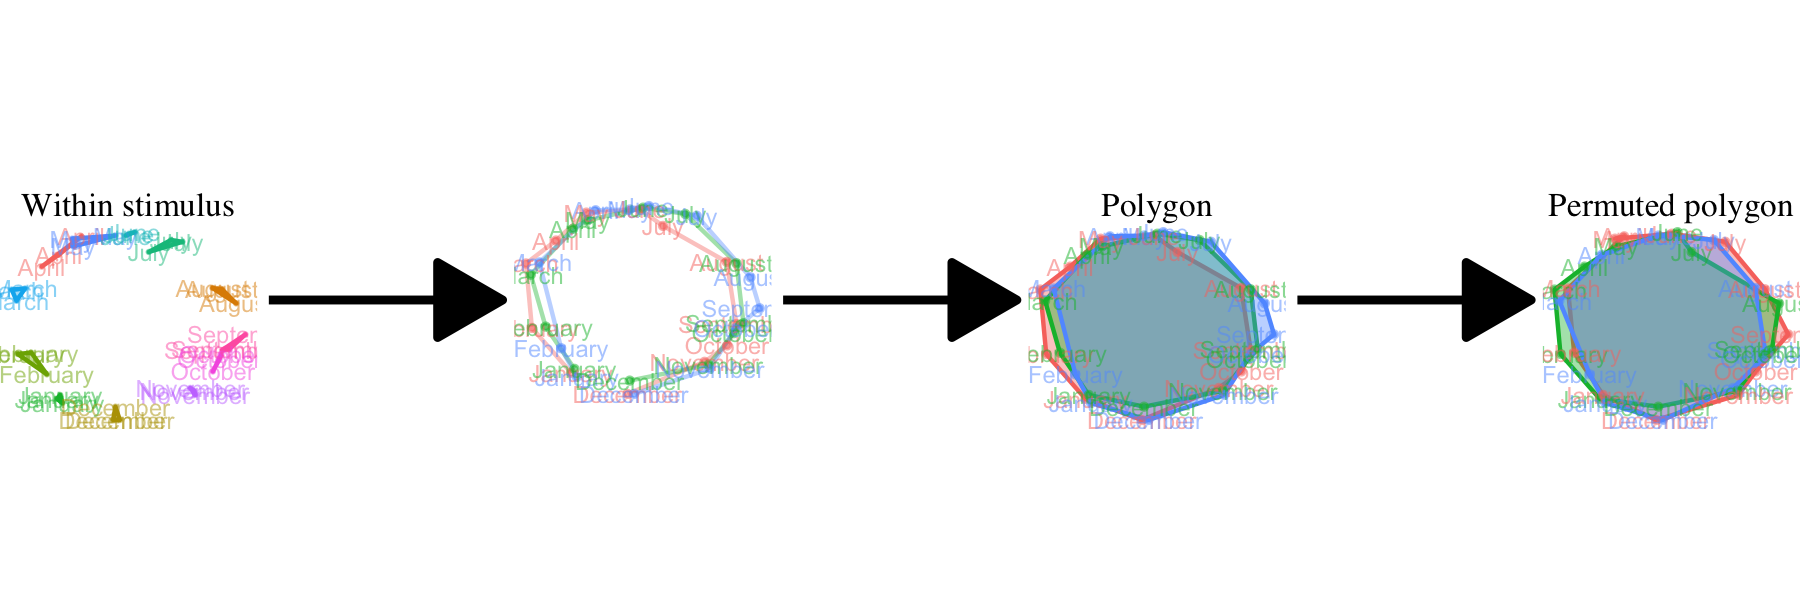
\includegraphics[keepaspectratio]{2.RegisteredReport_MS3_files/figure-pdf/fig-01-1.png}}

\noindent \emph{Note.} Example~of a participant's months space-form
illustrating the novel method's design.

\end{figure}

\section{Methods - phase I}\label{methods---phase-i}

Code and data for ``one-click'' reproducibility of this manuscript
including the following analyses are available on GitHub
(\url{https://github.com/remLach/SpaceSequenceSynDiagnostic}). All the
analyses are conducted in R, using the following packages `pROC' v.
1.19.0.1 (\citeproc{ref-pROC}{Robin et al., 2011}), `sf' v. 1.0.21
(\citeproc{ref-sf}{Pebesma \& Bivand, 2023}) and for visualization
`ggplot2' v. 4.0.1 (\citeproc{ref-ggplot2}{Wickham, 2016}),
`ggVennDiagram' v. 1.5.6 (\citeproc{ref-ggVennDiagram}{Gao \& Dusa,
2025}).

\subsection{Datasets and Participants}\label{datasets-and-participants}

To base the optimization of the consistency test on the largest possible
sample we looked for accessible datasets that used the same consistency
tasks on groups of synesthetes and controls. We found four datasets that
met these criteria. Two datasets were collected in laboratory settings
Rothen et al. (\citeproc{ref-rothen2016}{2016}) (see also
\href{https://osf.io/6hq94/files/osfstorage}{https://osf.io/6hq94}) and
Van Petersen et al. (\citeproc{ref-vanpetersen2020}{2020}) (see also
\url{https://data.ru.nl/collections/di/dcc/DSC_2018.00019_653}). The two
others came from on-line testing Ward (\citeproc{ref-ward2022a}{2022})
(see also \url{https://osf.io/nu5v4}) and an additional dataset was
provided by private communications with Jamie Ward. To match the other
datasets, stimuli of the weekdays and months categories were translated
from Dutch to English in the dataset from
(\citeproc{ref-vanpetersen2020}{Van Petersen et al., 2020}). For the
number category we included only digits from 0 to 9 that where presented
across all datasets (i.e.~excluding the stimuli ``50'' and ``100'' for
numbers in Van Petersen et al. (\citeproc{ref-vanpetersen2020}{2020})).

From the merged datasets, we kept 685 from the total 689 participants.
First, we excluded 0.02 \% empty trials (i.e.~skipped responses)
including trials flagged for having the same x or y coordinates across
categories and repetitions, causing the depletion (n = 2) participants
(as in \citeproc{ref-rothen2016}{Rothen et al., 2016};
\citeproc{ref-ward2018}{Ward et al., 2018}). (n = 2) participants were
excluded for having less than 4 coordinate points since polygons need at
least four coordinate. Note therefore, that 31 participants of the final
sample did not have responses in all three categories b\textless{}
repetition cases
\pdfcomment[icon=Check,color={0 0 1}]{NR11: I am not able to understand this sentence. I find the X confusing.}.
From the final sample of N = 685, 396 were self-reported synaesthetes
and 289 self-reported controls, see Table~\ref{tbl-01} and
Table~\ref{tbl-02}.
\pdfcomment[icon=Check,color={0 0 1}]{NR12: Based on self-reports?}

\begin{table}

{\caption{{Synesthetes}{\label{tbl-01}}}
\vspace{-20pt}}

\begin{longtable}[]{@{}llll@{}}
\toprule\noalign{}
Synaesthetes & Initial N & Final N & Age \\
\midrule\noalign{}
\endhead
\bottomrule\noalign{}
\endlastfoot
Rothen et al. (\citeproc{ref-rothen2016}{2016}) & 33 & 32 & 23.1 \\
Van Petersen et al. (\citeproc{ref-vanpetersen2020}{2020}) & 23 & 22 &
23.2 \\
Ward (\citeproc{ref-ward2022a}{2022}) & 252 & 252 & 37.2 \\
Ward 2 & 90 & 90 & NA \\
Total: & 398 & 396 & \\
\end{longtable}

\vspace{-20pt}
\noindent \emph{Note.} Synesthetes.~Demographics were not provided in
the dataset Ward 2. Before: before participant exclusion

\end{table}

\begin{table}

{\caption{{Controls}{\label{tbl-02}}}
\vspace{-20pt}}

\begin{longtable}[]{@{}llll@{}}
\toprule\noalign{}
Controls & Initial N & Final N & Age \\
\midrule\noalign{}
\endhead
\bottomrule\noalign{}
\endlastfoot
Rothen et al. (\citeproc{ref-rothen2016}{2016}) & 37 & 37 & 28.2 \\
Van Petersen et al. (\citeproc{ref-vanpetersen2020}{2020}) & 21 & 21 &
21.6 \\
Ward (\citeproc{ref-ward2022a}{2022}) & 215 & 213 & 19.9 \\
Ward 2 & 18 & 18 & NA \\
Total & 291 & 289 & \\
\end{longtable}

\vspace{-20pt}
\noindent \emph{Note.} Controls.~Demographics were not provided in the
dataset Ward 2. Before: before participant exclusion

\end{table}

Regarding the synaesthetes profiles, detailed participant information
such as questionnaire responses were only available from the two
datasets from the data by
\pdfcomment[icon=Check,color={0 0 1}]{NR13: delete Professor -> also further above where you mention how you obtained the data.}
Jamie Ward (i.e.~a majority of 573 participants). We described the
self-reported profiles for the stimulus categories used in the
consistency test (i.e.~number, weekdays and month), see
Figure~\ref{fig-02}.

\begin{figure}[!htbp]

{\caption{{Venn diagram of the types of self-reported
SSS}{\label{fig-02}}}}

\pandocbounded{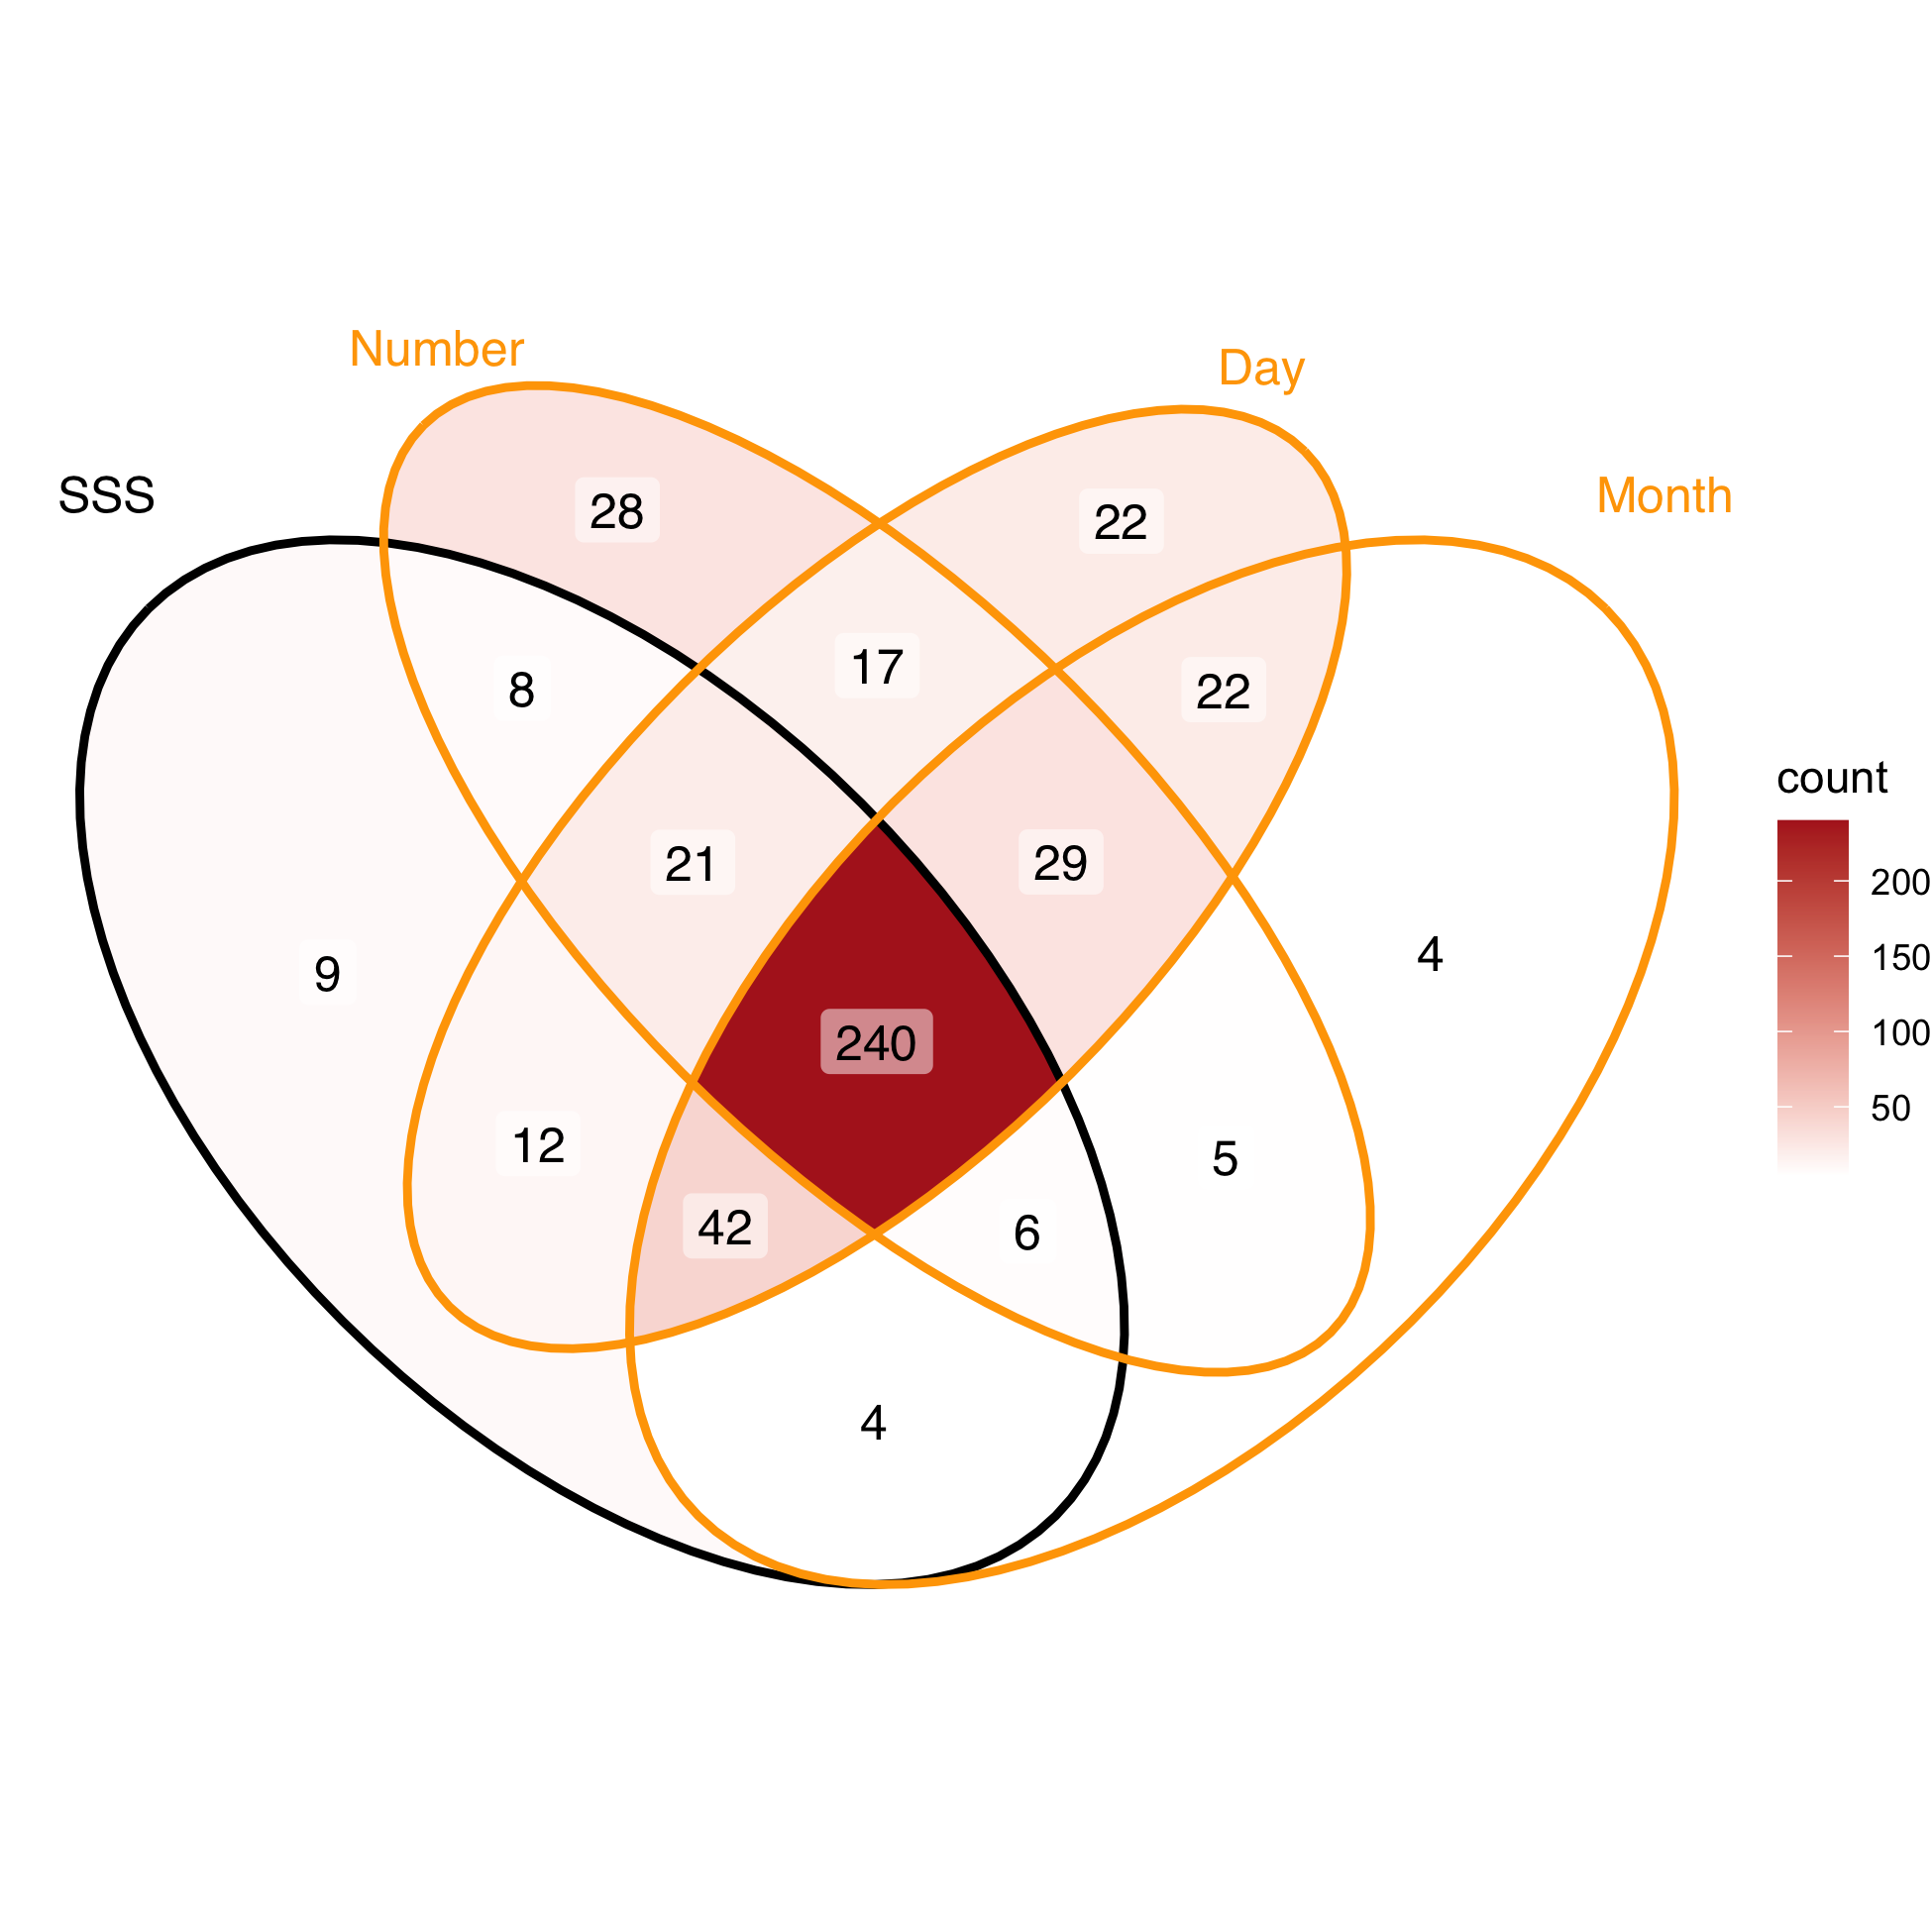
\includegraphics[keepaspectratio]{2.RegisteredReport_MS3_files/figure-pdf/fig-02-1.png}}

\vspace{-20pt}
\noindent \emph{Note.} Only~data from Pr. Ward is represented here. SSS
= Sequence-space synaesthesia

\end{figure}

\subsection{Procedure}\label{procedure}

\pdfcomment[icon=Check,color={0 1 0}]{CS1: I feel like there needs to be more detail here. So, in additon to what you already have - maybe some sample characteristics, data structure (number of reps per participant, number of stimuli), data preprocessing (any normalizations, handling missing data, inclusion and exclusion criteria), how you characterized the geometric spatial forms. I am not sure if this should Procedure or analysis but given this is a methods paper, I think maybe all this should come in the Procedure section?}

\pdfcomment[icon=Note,color={1 0 0}]{RL5: Some of the data preproessing on the participant and trial level are described just above together (since exluding trials can cause the exclusion of participants). Simce the analyses are on available data I tried to do as little pre-rpocesising as possible.}

For the consistency task, stimuli were presented randomly and
sequentially centrally on the screen. Participant were instructed to
click on the screen position where they visualize them. In Van Petersen
et al. (\citeproc{ref-vanpetersen2020}{2020}) and Rothen et al.
(\citeproc{ref-rothen2016}{2016}) the participants were allowed to skip
responses.

Stimuli included here were 7 weekdays (Monday to Sunday), 12 months
(January to December) and 9 numbers (0 to 9). For all the data from
Jamie Ward the stimuli were presented in randomized order with the
constraint that no stimulus was repeated until all unique stimuli (N =
29) had been presented once. The median display resolution was 1440 X
768, with a maximum of 2560 X 2025 and a minimum of 308 X 149.

\subsection{Analyses}\label{analyses}

\pdfcomment[icon=Note,color={1 0 0}]{RL6: All this part has been restructured and refrased.}

\pdfcomment[icon=Check,color={0 0 1}]{NR14: General comments: The method reads well, but is hard to follow because the methods you are using are complex. It might help to always using the same structure for each method. First, provide a theoretical motivation for the method -> replicate the original study, exploring the possiblity that mappings are not random but orientied at topological validity. Second, describe the method. Third, give a concrete example. I do not think you have done a bad job, but the results are too difficult to follow, because the reader needs to remember the methods.}

\pdfcomment[icon=Check,color={0 0 1}]{NR15: We need to think carefully, what could be done to make it easier to follow. It might also help here to always apply the same structure. First, refere to descriptive statistics -> The descriptive statistics for comparing the ROC across different methods can be found in Figure X. Second, describe what you want to test / theoretical motivation -> in order to test X, we conducted Y analysis. Third, describe what the test revealed. -> It showed that A was significantly higher than B. The things you are doing are complex. Therefore the reader needs careful guidance.}

\pdfcomment[icon=Note,color={1 0 0}]{RL7: This whole section has been rewritten and partically restructured. The structure of each method is: theory, method, example}

We first reproduced existing methods and test their classification
performances (i.e.~ability to class controls as controls and SSS as SSS)
using Receiver Operating Characteristics on the aggregated dataset. We
then compared these classification performances to the ones of novel
methods, see Figure~\ref{fig-01}.

\subsubsection{Reproduced consistency
tests}\label{reproduced-consistency-tests}

\pdfcomment[icon=Check,color={0 0 1}]{NR16: the subtitle seems confusing, it is not clear what you mean with on the stimulus level.}

We reproduced two existing consistency methods used to quantify the
spatial variability of responses between repetitions of the same stimuli
(\citeproc{ref-rothen2016}{Rothen et al., 2016};
\citeproc{ref-vanpetersen2020}{Van Petersen et al., 2020};
\citeproc{ref-ward2022a}{Ward, 2022}). Synaesethes relying on perceptual
spatial representations should have more consistent responses, hence
less variable (i.e.~closer) across the same stimuli across repetitions
than controls. Hence, variability was estimated by measuring the
distance between responses to the same stimuli (i.e. between repetitions
to the same stimuli, see first panel of Figure~\ref{fig-01}).

Formally the area (see Equation~\ref{eq-area}) and perimeter (see
Equation~\ref{eq-perim}) were calculated from the triangle (i.e.~given
three repetitions) formed by the \emph{x} and \emph{y} coordinates of
the three repetitions of each stimuli (i.e.~between the coordinates
\emph{(x1, y1), (x2, y2), (x3, y3)}).

\begin{equation}\phantomsection\label{eq-area}{
Area = \frac{|x1y2  +  x2y3  +  x3y1 \mathbin{-} x1y3 \mathbin{-}  x2y1 \mathbin{-} x3y2|}{2}
}\end{equation}

\begin{equation}\phantomsection\label{eq-perim}{
\begin{split}
Perimeter = \sqrt{(x2 \mathbin{-} x1)^2 + (y2 \mathbin{-} y1)^2} + \\ \sqrt{(x3 \mathbin{-} x2)^2 + (y3 \mathbin{-} y2)^2} + \\ \sqrt{(x1 \mathbin{-}  x3)^2 + (y1 \mathbin{-} y3)^2}
\end{split}
}\end{equation}

Each stimulus
\pdfcomment[icon=Check,color={0 0 1}]{NR17: stimuli is plural -> does not seem to make sense here. Should be singular.}
triangle area was then averaged by participants. The area metric is in
\% of the screen area to be able to compare with the consistency across
studies using different screen sizes. To account for screen size and
spread variability across the datasets and participants, area and
perimeter were also calculated on individually normalized \emph{x} and
\emph{y} coordinates (\emph{z-score}).

For example, if a participant's set of \emph{x,y} coordinates for Monday
are close to each other, then the triangle area and perimeter will be
smaller (i.e.~more consistent and characteristics of synaesthetes). The
recognized limit of this method, is that controls clicking on the same
position can achieve artificially high consistencies, see for example
the first four rows of Figure~\ref{fig-03}.

\begin{figure}[!htbp]

{\caption{{Example of extremes at the consistency
tests}{\label{fig-03}}}}

\pandocbounded{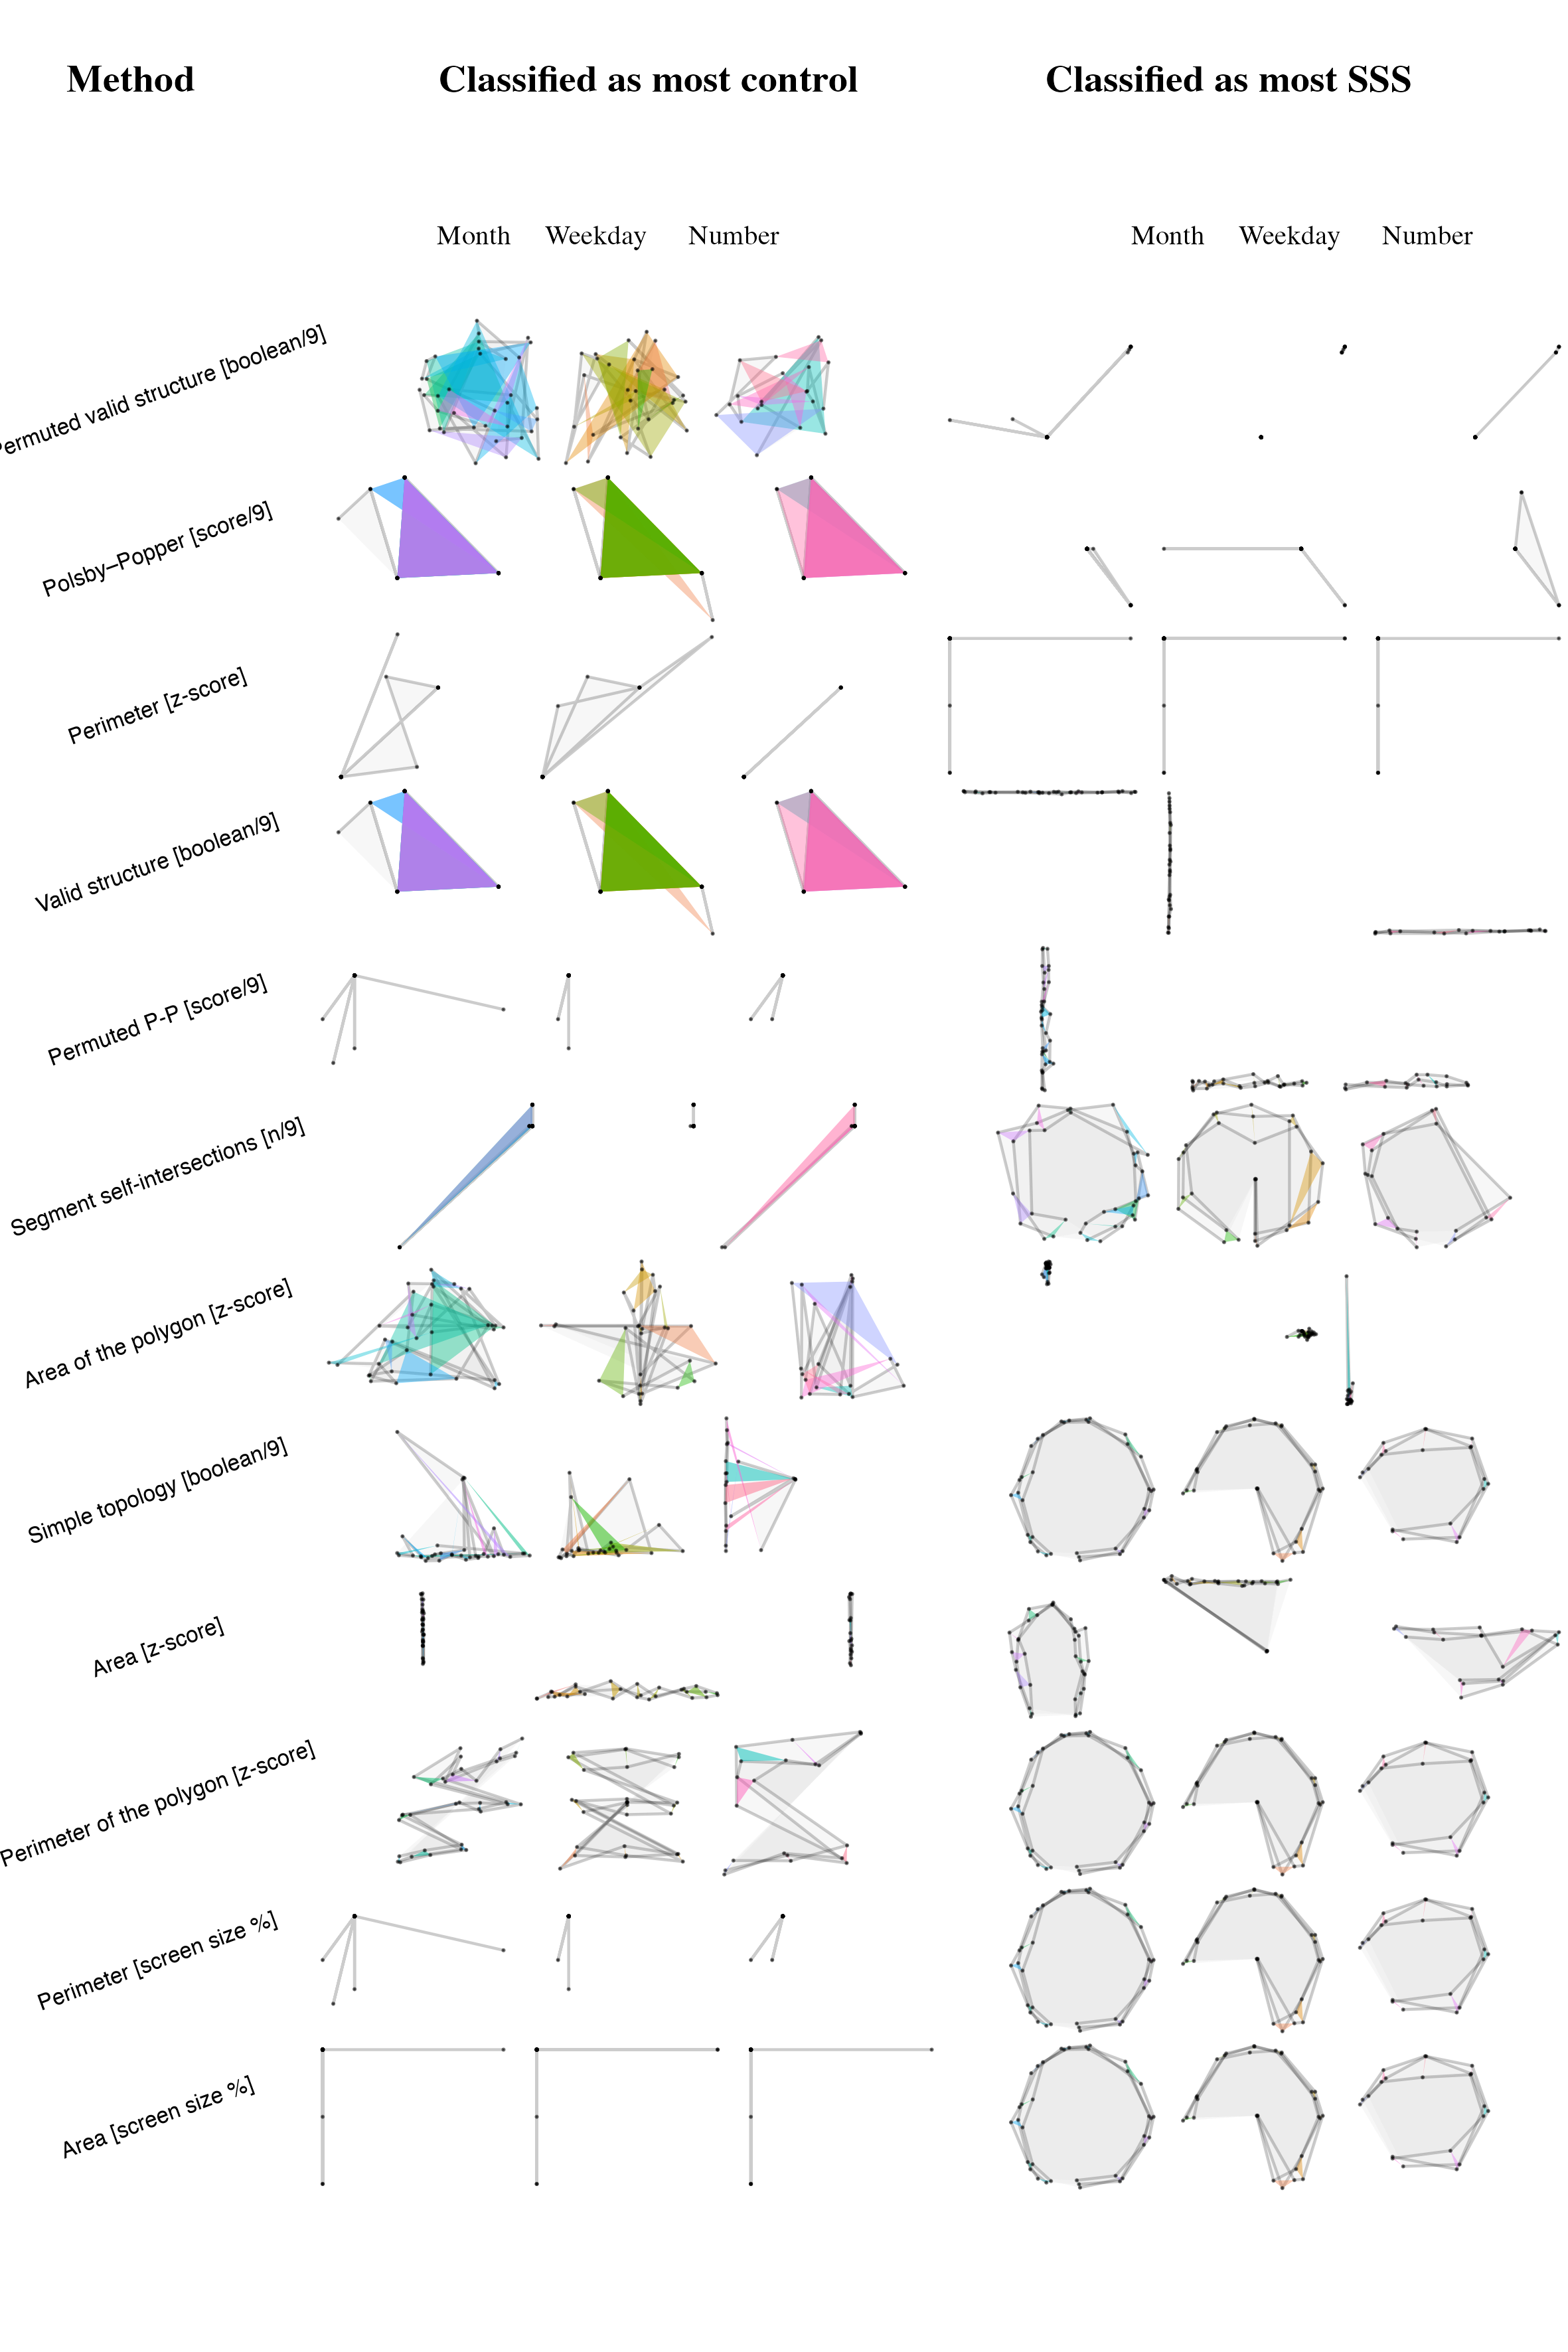
\includegraphics[keepaspectratio]{fig-03.png}}

\vspace{-20pt}
\noindent \emph{Note.} Plotted~are space-forms from the participants
that are the extreme of the consistency test's value

\end{figure}

\subsubsection{\texorpdfstring{Consistency tests on the \emph{space-form
level}}{Consistency tests on the space-form level}}\label{consistency-tests-on-the-space-form-level}

For the new methods for calculating consistency
\pdfcomment[icon=Check,color={0 0 1}]{NR18: do you mean new method of calculating consistency?},
we extracted geometrical features at the spatial-form level for each
repetition of sequentially ordered stimulus (i.e.~for numbers: 0
\texttt{→}1\texttt{→}2\texttt{→}3\texttt{→}4\texttt{→}5\texttt{→}6\texttt{→}7\texttt{→}8\texttt{→}9).
Each participant repeated each stimuli three times, leading to three
spatial-form per categories (numbers, weekdays and months) that is a
total nine space-forms per participants. Each space-form is evaluated
individually using different methods. Note that the stimuli forming the
space-forms are selected by the first time or repetition each one is
presented during the experiment (i.e.~Monday (repetition 1) \texttt{→}
Tuesday (repetition 1) \texttt{→} Wednesday (repetition 1), ect). The
rationale was that spatial-forms from SSS should have characteristic
geometrical properties that are distinct than control's ones. Later on
we extract the same geometrical properties on segments and polygons
where the repetitions labels are permuted within each categories
(i.e.~Monday (repetition 2) \texttt{→} Tuesday (repetition 1) \texttt{→}
Wednesday (repetition 3), ect). The rationale here is that spatial-forms
should have the same geometrical properties independently from
coordinate repetition order of the responses during the experiment.

Each space-form can be considered as a geometrical segment (i.e.~open
geometrical form) or polygon (i.e.~closed geometrical form) laying on 2D
Cartesian plane, similarly as originally described in Galton
(\citeproc{ref-galton1880}{1880}), see Figure~\ref{fig-01}.
\pdfcomment[icon=Check,color={0 0 1}]{NR19: for the above paragraph -> not clear what for each repetition means. do you mean trial 1 of each inducer of a given participant?}
Hence, we harnessed a geospatial analysis, the `sf' package version
1.0.21 (\citeproc{ref-sf}{Pebesma \& Bivand, 2023}) to extract polygons
and geometry-based features from participant's 2D (x,y) coordinate
responses. This package allows then, for example, to build and analyse
segments or polygons and then extract multiple geometrical descriptors
or features. Informed by the ordinality of the stimulus, we defined
segments and polygon by categories
\pdfcomment[icon=Check,color={0 0 1}]{NR20: not clear what you mean by conditions? -> stimulus type / category?}
and repetitions.

For example, Figure~\ref{fig-01}, shows how we can build segments and
polygons for months. This polygonal space-form has geometrical
properties that distinguishes it from random or pseudo-random responses.
For example, each of the three segments do not repeat.
Figure~\ref{fig-01} also illustrates the principle of permuting the
repetitions each of the three polygons are re-drawn using the stimuli
from different repetitions. For consistent space-forms the permutations
should lead to polygons with the same geometrical properties.

\paragraph{Segment
self-intersections.}\label{segment-self-intersections}

The first consistency test extracted from the segments is
self-intersection. Each space-form considered as ordered segments can
lead to different number of self-intersections. We reasoned that
responses from controls should be less structured leading to
self-intersections while for SSS the chances of self-intersections are
lower. In addition it addresses the issue of participants giving the
same responses, since with this test these responses would lead to a
large number of self-intersections and hence classification to control.

We considered the spatial-forms as a segment constituted by the lines
connecting consecutive stimuli separately for each category and
repetitions (i.e.~Monday (repetition 1) \texttt{→} Tuesday (repetition
1) \texttt{→} Wednesday (repetition 1), etc.) and then counted the
number of times each segment self-intersect. The number of
self-intersections were computed separately for each of the repetitions
\pdfcomment[icon=Check,color={0 0 1}]{NR21: each repetition or each of the repetitions?}
and categories and averaged per participants.

For example, Figure~\ref{fig-04} illustrate a participant with the sum
of self-intersections for each categories (columns) and repetitions
(rows). For the self-intersection test, this participants value would be
\(((4+1+2)+(2+1+0)+(3+0+0))/9 = 1.44\).

\begin{figure}[!htbp]

{\caption{{Example self-intersections test}{\label{fig-04}}}}

\begin{center}
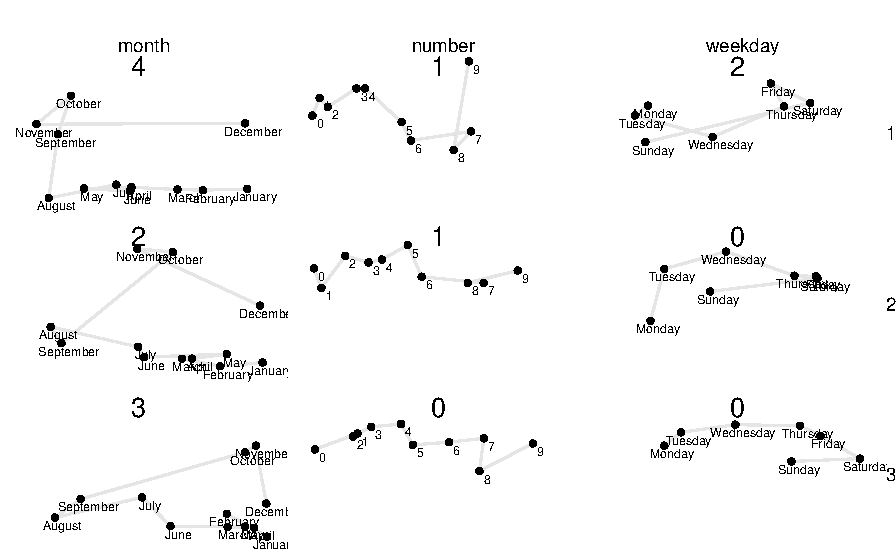
\includegraphics[width=0.5\linewidth,height=\textheight,keepaspectratio]{Fig04.pdf}
\end{center}

\vspace{-20pt}
\noindent \emph{Note.} Average~of the total number of self-intersections
across repetitions and categorie. In this example participant, the score
is \emph{1.44}

\end{figure}

\paragraph{Topological validity and
simplicity.}\label{topological-validity-and-simplicity}

We assessed topological propertries using geometric validation test. We
reasoned that space-forms from SSS should follow some topological rules
reflecting the ordinality properties of the stimulus. A direct analogy
comes from cartography, given spatial continuity underlying these
representations, they need to reflect some topological rules too.

\pdfcomment[icon=Note,color={1 0 0}]{RL8: I start with simplicity and then validity so we go from simple to more complex tests}

Similarly to the self-intersection test, topological simplicity
evaluates whether a geometric object has a simple structure without
self-intersections or self-tangencies. According to the OGC Simple
Features Specification (\citeproc{ref-herring2010}{Herring, 2010}), a
polygon boundary is considered simple if it does not pass through the
same point more than once (\citeproc{ref-postgis}{\emph{PostGIS 3.6.2dev
Manual}, n.d.}).

Topological validity tests if a polygons is well-formed and valid
according to the Open Geospatial Consortium (OGC) Simple Features
Specification (\citeproc{ref-herring2010}{Herring, 2010}). A polygon is
considered topologically valid if it satisfies the following criteria:
(1) if polygon rings are simple (i.e., they do not touch or
self-intersect), (2) boundary rings do not cross (3) boundary rings may
only touch points tangentially (4) rings that define holes are contained
within the exterior ring (5) the polygon rings must not split the
polygon (\citeproc{ref-postgis}{\emph{PostGIS 3.6.2dev Manual}, n.d.}).
\pdfcomment[icon=Check,color={0 0 1}]{NR22: there is some repetition}
Note that simplicity is a condition for validity: a polygon can be
simple but still invalid (e.g., if an interior ring extends outside the
exterior ring).

Topological simplicity and validity evaluates each space form with a
binary outcome (0 = is simple/valid, 1 = complex/invalid).Topological
validity and simplicity was tested across individual 3 categories
(weekdays, month and numbers)
\pdfcomment[icon=Check,color={0 0 1}]{NR23: sometimes you seem to call it conditions and now categories. Be consistent with terminology.}
and 3 repetitions, hence 9 space-forms or polygons.

For the example of a participant, having all weekday's space-froms
polygons being invalid across repetitions (i.e.~1,1,1), all month's
being invalid (i.e.~0,0,0), and numbers invalid in one of the three
repetitions (0,1,0), then the topological validity score would be 4/9 ≈
0.44. Hence, validity and simplicity of each participants span from 1
(all 9 are valid/simple) to 0 (none of the 9 forms are valid/simple).
\pdfcomment[icon=Check,color={0 0 1}]{NR24: the example helps a lot, maybe add a concrete example for all methods.}

\paragraph{Compactness score.}\label{compactness-score}

We then implemented a compactness score of the space-formed polygons. We
used the score developed to quantify the gerrymandering of political
district Polsby and Popper (\citeproc{ref-polsby1991}{1991}). In the
context of geopolitics, gerrymandering is a politically motivated
strategy of redefining electoral district's boundaries to advantage a
political party. As a consequence, the compactness of districts
redefined by political motivations are less likely to be compact than if
they would follow geomorphological properties. We expected SSS
space-form polygons to be more compact for SSS than controls since those
polygons are grounded in a perceptual space.

The compactness score is calculated as the ratio of the area and
perimeter of a polygon. Formally, the Polsby--Popper score is calculated
from the polygon's area and perimeter Equation~\ref{eq-PP}:

\begin{equation}\phantomsection\label{eq-PP}{
P - P\ score = \frac{4\pi \cdot Area}{Perimeter^2}
}\end{equation}

Hence, this score ranges from 1 (maximally compact) to 0. For
space-forms that have an area of 0 (for example when all the responses
are in the same position), the score could not be computed, we therefore
re-defined those polygon's p-p score to 1.

For example, for a polygon overlapping to a perfect circle, the
polsby-popper score would be 1. Indeed, the maximal participant's scores
displays circular space-form, see Figure~\ref{fig-03}.

\paragraph{Permutation-based feature
extraction.}\label{sec-permutation-based-feature-extraction}

If synesthetic forms are truly consistent, they should remain stable
independently of the experimental order in which the stimulus is
presented, see Figure~\ref{fig-01}. Hence, we re-calculated the three
most performant tests (i.e.~leading to higher Area under the Curve) by
permuting the repetition order within each condition (see
Section~\ref{sec-permutation-based-feature-extraction}). We predicted
that this permuted-based consistency would yield to better
classification performance (higher AUC values) compared to non-permuted
methods.

Each permutation was obtained by shuffling the repetition order or label
between stimulus presentation (i.e.~Monday (repetition 2) \texttt{→}
Tuesday (repetition 3) \texttt{→} Wednesday (repetition 1), ect.). Then
we extracted the geometrical feature from x,y coordinates of stimuli
from the same categories in non-chronological order. We repeated 500
permutations per participants and averaged the permuted distributions to
obtain a single permutation score per participant. The permutation
scores were calculated for topological validity and Polsby--Popper
score.

For example, segments for weekdays were constructed with the x,y
coordinates randomly permuted across repetition order, i.e.~Monday
(repetition 1), Tuesday (repetition 3), Wednesday (repetition 2), ect.,
see rightmost panel of Figure~\ref{fig-01}.

\subsubsection{Receiver Operating Characteristic
analyses}\label{sec-receiver-operating-characteristic-analyses}

Each of the previous method's performance in classifying SSS from
controls was compared with Receiver Operating Characteristics (ROC)
analyses. Classification performance was quantified using the area under
the curve (AUC), with higher AUC values indicating better discrimination
between SSS and control groups. The optimal cutoffs were calculated
using Youden's index (\citeproc{ref-youden1950}{Youden, 1950}).
Discriminant Power (DP) was used as an additional estimate of
discrimination performance according to the optimal cutoff
(Equation~\ref{eq-DP}). DP around 1 being interpreted as inefficient
discrimination.

\begin{equation}\phantomsection\label{eq-DP}{ 
DP = \frac{\sqrt{3}}{\pi} (\log(\frac{sensitivity}{1−sensitivity}) + \log(\frac{specificity}{1−specificity}))  
}\end{equation}

The statistical comparison of ROC curves between the methods was
operated testing the difference of AUC between pairs of curves using
bootstrapping method (1000 iterations) since it allows to compare
methods with different directions. Each bootstrap results in the
subtraction of the AUC between the two ROC. Then the each of the AUC
difference's (D) are divided by the standard deviation of those
difference and compared to a normal distribution (Equation~\ref{eq-D}).

\begin{equation}\phantomsection\label{eq-D}{
D = \frac{AUC_1-AUC_2}{SD}
}\end{equation}

Therefore we statistically compared all the AUC of each method
\pdfcomment[icon=Check,color={0 0 1}]{NR25: methods or method?} as the
difference to the highest AUC method.

\section{Results - phase I}\label{sec-results}

\pdfcomment[icon=Check,color={0 1 0}]{CS2: I think this section is a little confusing to read because you talk about ROC and AUC, but then also DP. But then you go back to talking about ROC and AUC and it is a little unclear how DP fits into the story.}

\pdfcomment[icon=Check,color={0 0 1}]{NR26: The results section until the discussion of the present study is quite hard to follow. It requires simplification}

Regarding the reproduced consistency test, the available datasets
resulted in descriptively different averages for SSS, see
Table~\ref{tbl-04}. The triangle area (in \% screen size) for SSS was
surprisingly larger in the present aggregated dataset 0.26\% (\emph{SD =
0.52\%}) than in previous studies studies: 0.14\% (\emph{SD = 0.13\%})
in Rothen et al. (\citeproc{ref-rothen2016}{2016}) and 0.14\% (\emph{SD
= 0.17}\%) in Ward et al. (\citeproc{ref-ward2018}{2018}). Descriptives
break down by dataset (see \hyperref[apx-SM2byds]{Appendix~B}) suggest
that the dataset with the largest number of participants
(\citeproc{ref-ward2022a}{Ward, 2022}) is driving this difference
(i.e.~with an area of 0.26\%, see Table~\ref{tbl-apx02}). It is
important to note that since each method uses different metrics, these
cannot directly be compared to each others. Hence the rightmost columns
of Table~\ref{tbl-04} also reports standardized z-score descriptives
allowing comparison across different metrics. Furthermore note some the
directionality differs between the methods (i.e.~the area method is
expected to be smaller for SSS in contrast to validity methods that are
expected be larger for SSS).

\begin{table}

{\caption{{Descriptive values of each test per group}{\label{tbl-04}}}
\vspace{-20pt}}

\fontsize{12.0pt}{14.0pt}\selectfont
\begin{tabular*}{\linewidth}{@{\extracolsep{\fill}}lrrrr}
\toprule
Feature & Control & SSS & Control [zs] & SSS [zs] \\ 
\midrule\addlinespace[2.5pt]
Area [screen size \%] & 0.46 (0.87) & 0.26 (0.52) & 0.17 (1.25) & -0.12 (0.75) \\ 
Area [z-score] & 0.26 (0.32) & 0.08 (0.14) & 0.42 (1.29) & -0.30 (0.55) \\ 
Perimeter [screen size \%] & 0.03 (0.03) & 0.03 (0.08) & 0.03 (0.44) & -0.02 (1.26) \\ 
Perimeter [z-score] & 3.30 (1.72) & 1.59 (1.16) & 0.60 (1.04) & -0.44 (0.70) \\ 
Segment self-intersections [n/9] & 9.56 (11.31) & 1.87 (5.42) & 0.48 (1.23) & -0.35 (0.59) \\ 
Area of the polygon [z-score] & 1.00 (0.99) & 1.91 (1.31) & -0.42 (0.79) & 0.30 (1.03) \\ 
Perimeter of the polygon [z-score] & 9.49 (3.44) & 8.39 (2.48) & 0.21 (1.16) & -0.16 (0.83) \\ 
Simple topology [boolean/9] & 0.22 (0.23) & 0.40 (0.27) & -0.39 (0.85) & 0.28 (1.01) \\ 
Valid structure [boolean/9] & 0.13 (0.19) & 0.39 (0.28) & -0.54 (0.69) & 0.39 (1.01) \\ 
Permuted valid structure [boolean/9] & 0.12 (0.16) & 0.36 (0.25) & -0.57 (0.64) & 0.41 (1.01) \\ 
Polsby–Popper [score/9] & 0.11 (0.13) & 0.27 (0.19) & -0.52 (0.69) & 0.38 (1.02) \\ 
Permuted P-P [score/9] & 0.11 (0.17) & 0.41 (0.33) & -0.56 (0.56) & 0.40 (1.06) \\ 
\bottomrule
\end{tabular*}
\begin{minipage}{\linewidth}
\vspace{.05em}
Note: mean (standard deviation) of all the consistency tests. The two rightmost columns display the same descriptives in z-score transformed values, enabling comparison across different metrics. Z-scores were calculated for all participants, separately for each test.\\
\end{minipage}

\end{table}

In sum, the descriptives stress out the variability across datasets and
the need for additional analyses from phase II. It also stresses out the
use of methods that are either standardized or that do not rely on
metrics that depend on the experimental settings.

\subsection{ROC analyses}\label{roc-analyses}

The results of the ROC analyses are summarized in Table~\ref{tbl-03} and
Figure~\ref{fig-05}. The consistency methods are sorted by highest Area
Under the Curve (AUC). We applied statistical comparisons of all the ROC
curves by pairs. We compared the permuted validity method that lead to
the highest AUC as described in
Section~\ref{sec-receiver-operating-characteristic-analyses}. All
p-values are adjusted with false discovery rate.

\begin{figure}[!htbp]

{\caption{{Receiver Operating Characteristic (ROC) curves of all
tests}{\label{fig-05}}}}

\pandocbounded{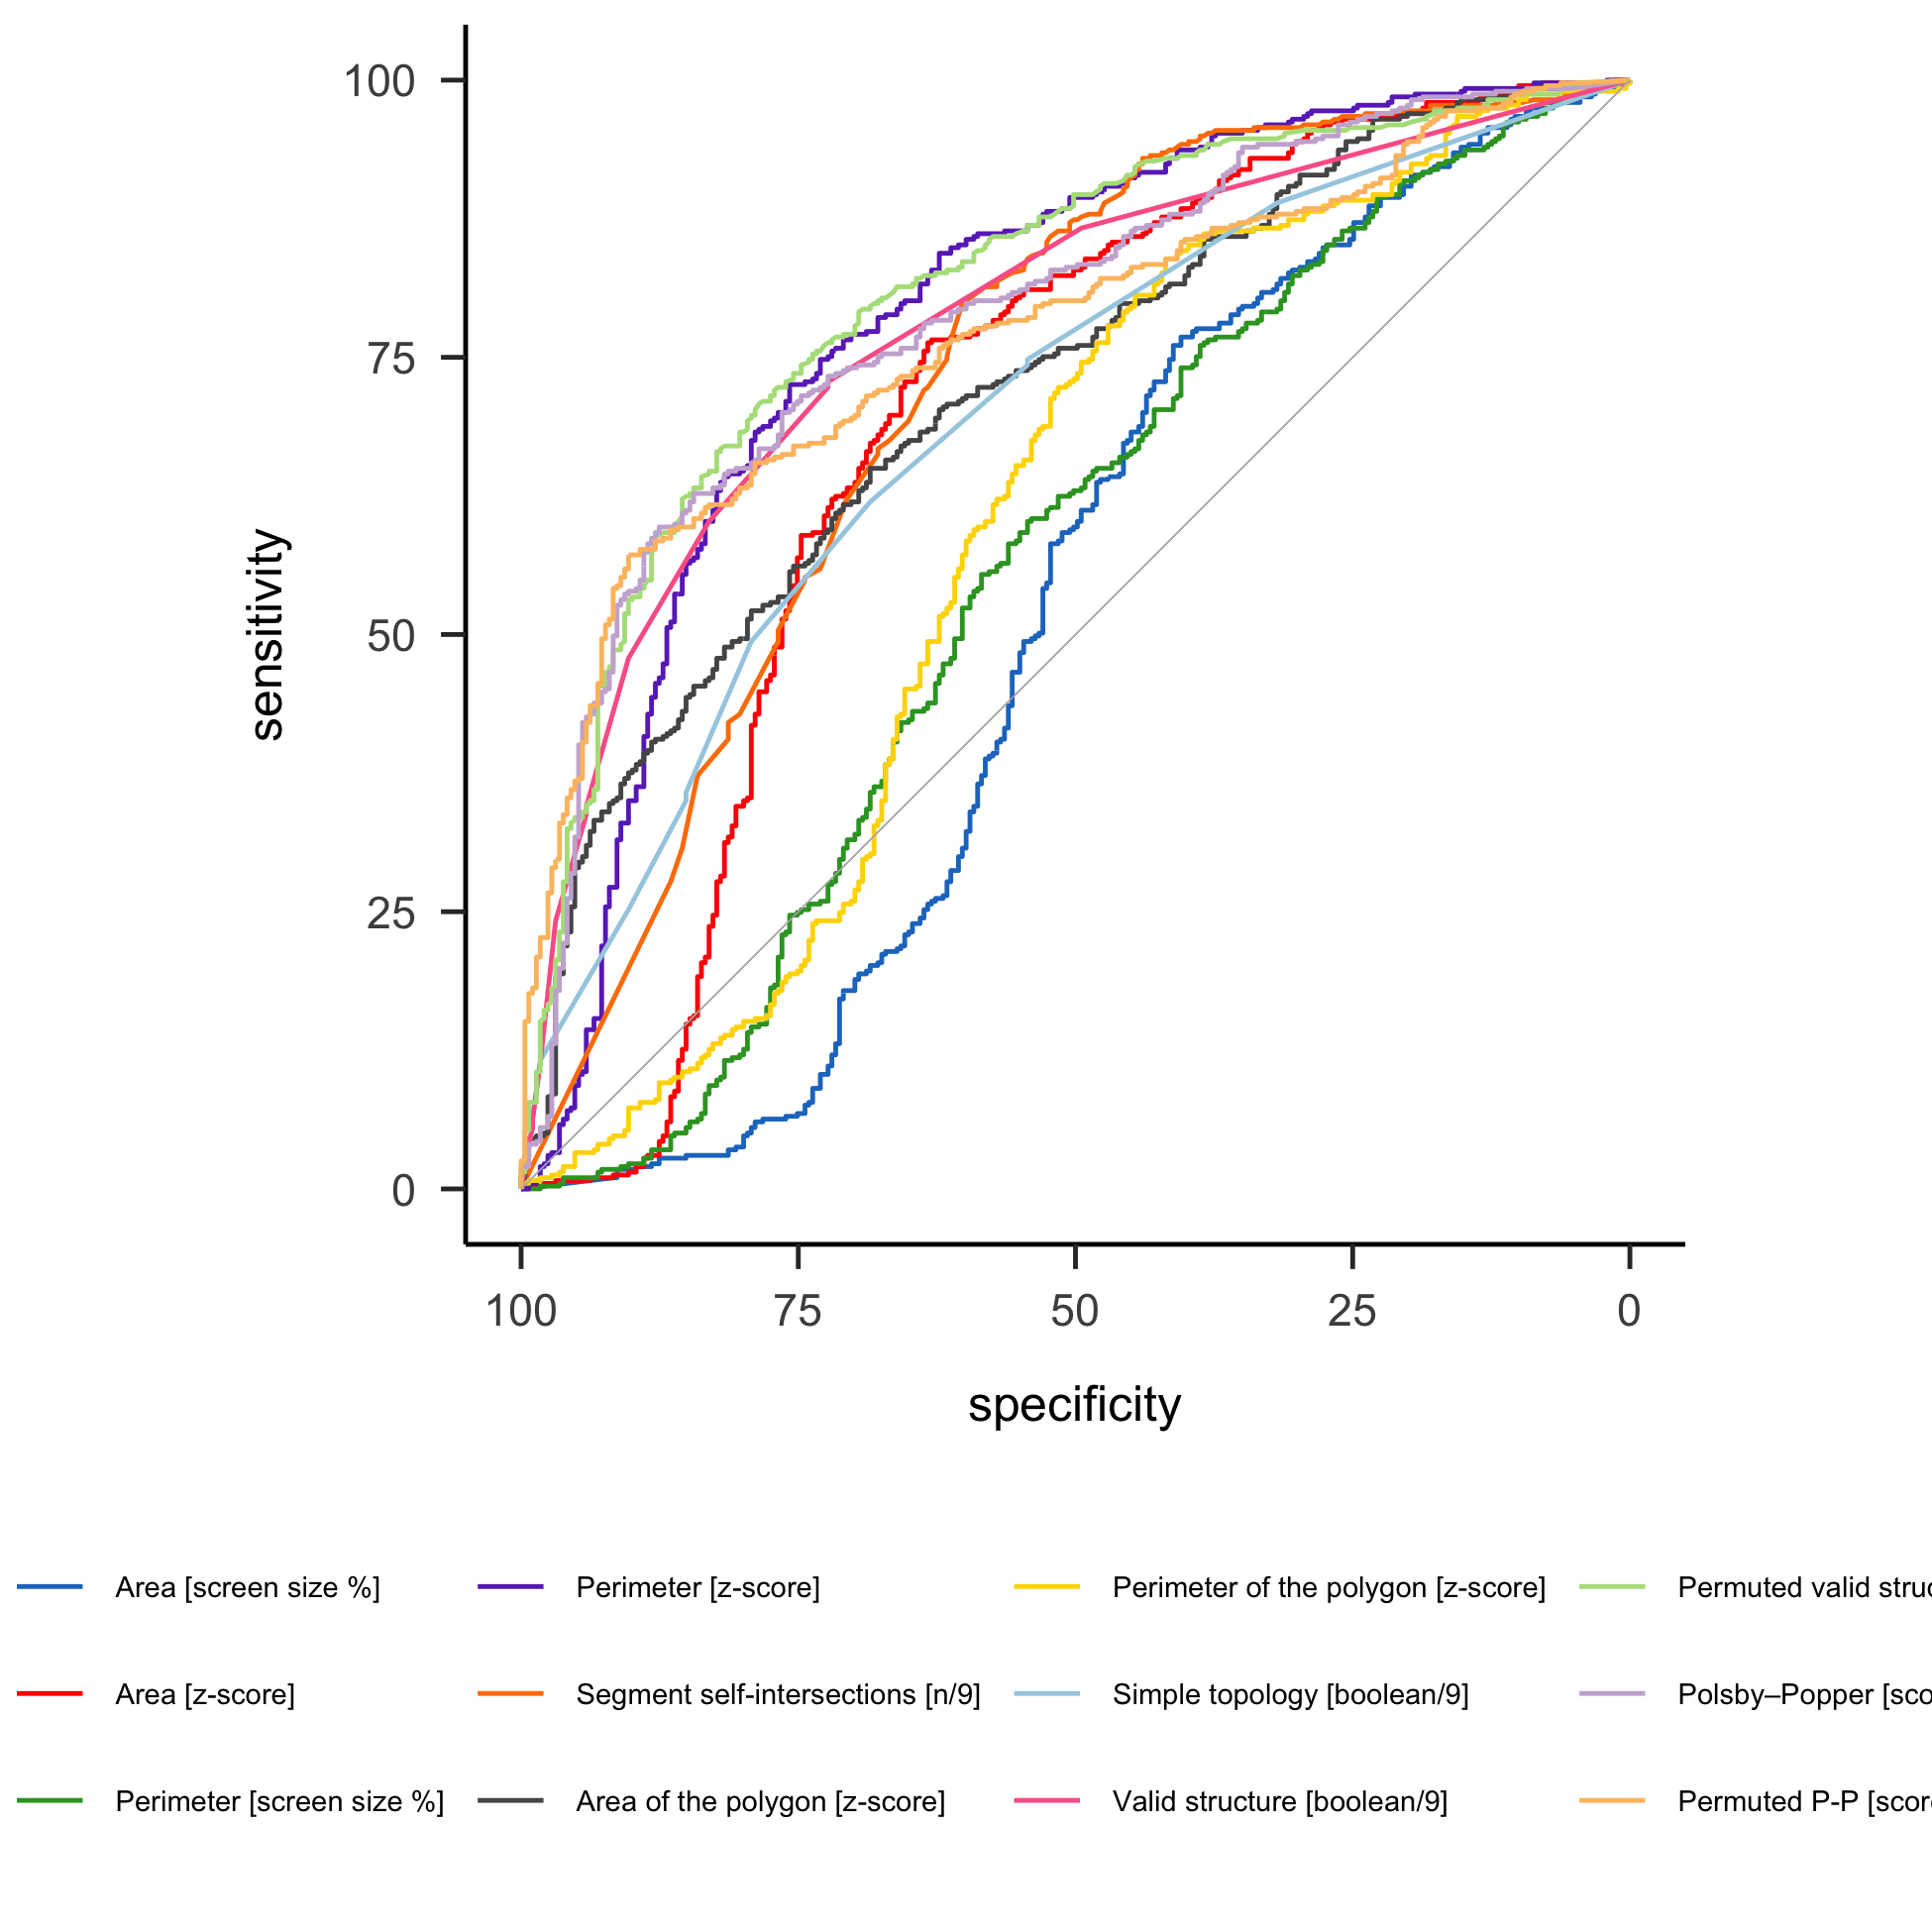
\includegraphics[keepaspectratio]{2.RegisteredReport_MS3_files/figure-pdf/fig-05-1.png}}

\vspace{-20pt}
\noindent \emph{Note.} Grey~line indicates chance level

\end{figure}

\begin{table}

{\caption{{ROC analyses of all tests}{\label{tbl-03}}}
\vspace{-20pt}}

\fontsize{12.0pt}{14.0pt}\selectfont
\begin{tabular*}{\linewidth}{@{\extracolsep{\fill}}lrrrrr}
\toprule
Feature & AUC & DP & threshold & sensitivity & specificity \\ 
\midrule\addlinespace[2.5pt]
Permuted valid structure [boolean/9] & 81.16 & 2.13 & 0.17 & 70.78 & 78.55 \\ 
Polsby–Popper [score/9] & 78.96 & 2.29 & 0.19 & 59.70 & 87.54 \\ 
Perimeter [z-score] & 78.80 & 2.06 & 1.73 & 72.54 & 75.78 \\ 
Valid structure [boolean/9] & 78.12 & 1.90 & 0.14 & 72.80 & 72.32 \\ 
Permuted P-P [score/9] & 77.14 & 2.46 & 0.20 & 57.18 & 90.31 \\ 
Segment self-intersections [n/9] & 72.93 & 1.75 & 1.17 & 79.85 & 60.21 \\ 
Area of the polygon [z-score] & 72.03 & 1.36 & 1.29 & 64.99 & 68.51 \\ 
Simple topology [boolean/9] & 69.74 & 1.24 & 0.28 & 61.96 & 68.51 \\ 
Area [z-score] & 69.27 & 1.68 & 0.08 & 76.32 & 63.32 \\ 
Perimeter of the polygon [z-score] & 59.12 & 1.29 & 10.46 & 83.88 & 41.87 \\ 
Perimeter [screen size \%] & 55.34 & 0.68 & 0.03 & 76.07 & 38.75 \\ 
Area [screen size \%] & 50.87 & 0.79 & 0.21 & 76.83 & 40.48 \\ 
\bottomrule
\end{tabular*}
\begin{minipage}{\linewidth}
\vspace{.05em}
AUC = Area Under the Curve. DP = Discrimination Power.\\
\end{minipage}

\end{table}

Permuted validity and the standardized perimeter led to the highest AUC
and were statistically the same (\emph{D} = 1.4, \emph{p = n.s.}). The
Polsby-Popper method, did statistically differ from the permuted
validity (\emph{D} = 2.03, \emph{p} \textless{} .05), while
counter-intuively having descriptively larger AUC than the standardized
perimeter test, see Table~\ref{tbl-03}. All the other tests led to
significantly smaller AUC than permuted validity (i.e.~all \emph{D}
\textgreater{} 3.18, \emph{p} \textless{} .01).

We conducted further analyses to compare the sensitivity and specificity
of the Polsby-Popper to the permuted validity that resulted in no
significant differences. Permuted validity and Polsby-Popper method did
not differ in specificity (at a sensitivity of 80\%, \emph{Z =} 0,
\emph{p} = \emph{n.s.}). However, comparing specificity to the
standardized perimeter resulted in higher specificity for the
Polsby-Popper method (at a sensitivity of 80 \%, \emph{D =} 2.04,
\emph{p} \textless{} .05). For sensitivity, the Polsby-popper method did
not differ neither from permuted validity (at a specificity of 80\%,
\emph{D =} 1.06, \emph{p} = \emph{n.s.}) nor from perimeter (at a
specificity of 80\%, \emph{D =} 0.98, \emph{p = n.s.}). See also
Figure~\ref{fig-apx01} for the density plot's distribution across
self-reported SSS and controls.

The results also show that the permutations significantly improved the
AUC for topological validity (\emph{D} = 3.18, \emph{p} \textless{}
.01). Post-hoc comparison of the Polsby-Popper method to it's permuted
counterpart indicate (one-sided bootstrap comparison of the AUC:
\emph{D} = -1.78, \emph{p} \textless{} .05). In sum, the permutations
only selectively improved classification performances of topological
validity but not the compactness Polsby-Popper score.

In conclusion for the statistical analyses, while the permuted validity
and standardized perimeter lead to overall higher AUC than the
Polsby-Popper, the later resulted in significantly higher sensitivity
than perimeter (i.e.~better probability of detecting SSS) than
standardized perimeter, see Table~\ref{tbl-03}. Hence the permuted
validity, standardized perimeter and Polsby-Popper were the most optimal
consistency methods for the aggregated dataset.

The cut-off leading to the most optimal classification for the permuted
validity score is: 0.17 corresponding to 1.53 valid of 9 forms. The
cut-off leading to the most optimal classification for standardized
perimeter is: 1.73 of individual \emph{z-scores}. The cut-off that leads
to the most optimal classification with the compactness score obtain
from the Polsby-Popper method is: 0.19, the compactness score is
calculated on the space-form polygon's area and permimeter using
Equation~\ref{eq-PP}.

In sum, the novel permuted validity method and Polsby-Popper compactness
score resulted in comparable classification performances between
controls and SSS to the standardized coordinate's perimeter method.

\subsection{Further analyses}\label{further-analyses}

We conducted further analyses by sub-sampling the dataset source and
questionnaire percentiles, see Appendixes. The first aim of these
analyses was to test the stability of the classifications from different
methods across experiments (i.e.~datasets) and sample characteristics
(i.e.~questionnaire scores).
\textcolor{teal}{The second aim was to describe the false positves and negatives of each tests to check for some biases towards some space-forms or responses in the same position}.
We also used a correlational approach to test for correlations between
method's metrics and questionnaires.

We sub-sampled the dataset source for the five most optimal tests (i.e.
higher AUC) and recalculated AUC, sensitivity and sensibility. We found
similar values for the different datasets, see Figure~\ref{fig-apx02}.
The density plots also seem to support bimodal distributions by datasets
Figure~\ref{fig-apx03}.

Including only the data by Jamie Ward, we sub-sampled the participants
depending on the percentiles of the questionnaire scores , taking the
10\% highest questionnaire scores against the 10 \% lowest (i.e.~90-100
\%). Here also most of the values remain relatively stable independently
from the questionnaire distribution of the samples, see
Figure~\ref{fig-apx04}. Another important point addressed in the
literature about consistency test is circularity.

The circularity is given in that if consistency tests are used to
classify SSS and controls, then those groups will by definition differ
in consistency (\citeproc{ref-root2025}{Root et al., 2025}). Hence, we
made a correlation matrix with the questionnaire scores and all the
tests, see Appendix. The two highest correlations are indeed between the
questionnaire score and perimeter (r = .58) and permuted validity (r =
.50), see Figure~\ref{fig-apx05}.

\pdfcomment[icon=Note,color={1 0 0}]{RL9: This is new:}We developed an
averaging approach to visualize the space-forms across all participants
by groups (SSS vs controls) and categories (month, number and weekday).
The figure in the appendix (Figure~\ref{fig-apx06}), shows more circular
patterns for months and more linear horizontal and vertical for numbers.
We used the averaging approach to visually qualify the false negatives
(Controls classified as SSS) and positives (SSS classified as controls)
of each consistency test. Descriptively, the perimeter test seems to
classify linear responses for numbers as controls compared to the other
methods.

Finally, some of the participants might have been originally
mis-attributed to control or SSS or there might be consistent controls
and inconsistent synesthetes (\citeproc{ref-eagleman2007}{Eagleman et
al., 2007}; see \citeproc{ref-root2025}{Root et al., 2025}), see
Figure~\ref{fig-apx07}. We found \textasciitilde6\% of the full sample's
synesthetes to be consistently classified as controls (i.e.~consistent
false negatives) by the five methods with the highest AUC, see
Figure~\ref{fig-apx08}. \textasciitilde3 \% controls are consistently
classified as SSS (i.e.~consistent false positives)
Figure~\ref{fig-apx09}. Qualitatively, the consistent false negative
seem not to be like

In sum, these further analyses evidence first, some variability across
datasets. Second, the main consistency tests seems to stably classify
more extreme groups of SSS and controls than less extremes ones (based
on questionnaire score distribution). Third, qualitatively less
false-positives (SSS classified as controls) for the novel space-form
methods (i.e.~validity and compactness) than the old perimeter method.
Fourth, we identified a group within the controls who systematically
pass all the consistency tests and a group within the SSS who
systematically fail all consistency test, accounting for about 9\% of
all participants.

\section{Methods - phase II}\label{sec-phase-ii-methods}

Additional data will be collected in the future using the same
consistency test, with the procedural exception that there will be four
repetitions per stimuli instead of three ( Sachdeva et al.
(\citeproc{ref-sachdeva2024}{2024}), Stage 1 in-principle acceptance).
Hence for the stimulus levels tests we will compare the area and
perimeter of a quadrilateral of four coordinates pairs instead of a
triangle. Materials are more details on this study are pre-registered on
OSF, including ample size and recruitment method
(\citeproc{ref-sachdeva2024}{Sachdeva et al., 2024}, Stage 1
in-principle acceptance) (see also \url{https://osf.io/6wn4m}).

\section{Discussion - phase I}\label{discussion---phase-i}

\pdfcomment{CS3: I don’t think you need any of the sections from here onwards for a pre-registration/registered report However, saying this, I think you can move some bits of the discussion section into the results section.I do not think you should discuss limitations right now}

Our investigation of four datasets found two main consistency tests
leading to the optimal classification of SSS from control: standardized
perimeter between stimulus repetitions and permuted topological validity
on the space-form level.

Further analyses show variabilities between the test's AUC exists
depending on the dataset source, which could explain why we could not
replicate Rothen et al. (\citeproc{ref-rothen2016}{2016})'s area but
rather found the perimeter as a more optimal test. The stability across
varying percentiles of the synaesthesia questionnaire's score suggest
the tests work as well for more marked forms of SSS (note however that
this analysis was limited to Jamie Ward's data). The standardized
perimeter also leads to slightly higher correlation with the
questionnaire scores (r = .57) than permuted topological validity (r =
.51), see Figure~\ref{fig-apx05}.

In sum, while we could prove similar performances using a different
approach based on the space-form level (i.e.~topological validity), we
found similar classification performances than using stimulus-repetition
level test such as perimeter.

\subsection{Limitations}\label{sec-limitations}

Although an optimal test to classify SSS might be particularly relevant
for experimental purposes, several important limitations need to be
considered. First, consistency tests contain only a limited set of
sequential stimuli (i.e.~months, weeks and the first ten natural
numbers) that could potentially elicit synaesthetic experiences. Other
ordinal categories such as temperature, clock time, musical keys might
be more relevant for some individuals with SSS. For numbers
specifically, better consistency tests might be obtained using a larger
set size (i.e.~including decades and hundreds), as descriptively
interesting form changes occur at different decimals in base-10 number
systems (\citeproc{ref-galton1880}{Galton, 1880}).

Second, the use of diagnostic cutoffs assumes categorical distinctions
between groups, but SSS may exist on a continuum and scores might be
more suitable (\citeproc{ref-price2013}{Price \& Pearson, 2013}). This
limitation is related to the circularity mentioned previously:
diagnostic cutoffs as calculated here depend on how SSS and controls are
classified in the first place (\citeproc{ref-simner2012}{Simner, 2012}).
Measures of other characteristics of synaesthesia such as automaticity
or visual Gabor detection might be necessary to establish external
validity (\citeproc{ref-ward2018}{Ward et al., 2018}). Indeed,
determining the prevalence of SSS in the general population requires
definitional choices that might be based on more conservative or lenient
criteria (\citeproc{ref-brang2010}{Brang et al., 2010};
\citeproc{ref-jonas2014}{Jonas \& Price, 2014};
\citeproc{ref-sagiv2006}{Sagiv et al., 2006};
\citeproc{ref-ward2018}{Ward et al., 2018}). These difficulties are
reflected in the span of current prevalence estimates of SSS: 4.4 \%
(\citeproc{ref-brang2013}{Brang et al., 2013}), 8.1 \%
(\citeproc{ref-ward2018}{Ward et al., 2018}) and 14 \%
(\citeproc{ref-seron1992}{Seron et al., 1992}).

Third, as shown in Figure~\ref{fig-apx02}, we find that the optimal
criteria can vary across datasets. In other word, we obtain different
AUC depending on the datasets. These differences might be explained by
different sampling methods biases, for example
(\citeproc{ref-vanpetersen2020}{Van Petersen et al., 2020}) recruited
SSS from over one hundred candidates to maximise participant reporting
synesthetic experiences.

\pdfcomment[icon=Note,color={1 0 0}]{RL10: Removed paragraph: Another possible explanation may be methodological and related to the option to skip responses in the task, leaving empty cases for some participants. Indeed, having fewer responses (i.e., fewer coordinates) increases the likelihood of producing a valid spatial form also in controls. Conversely, perimeter and area are differentially affected by missing responses. It is also possible that SSS are not actually inconsistent [@root2025; @eagleman2007] or that non self-reported SSS are consistent [@itoh2024]. Another possibility might have to do with the original classification of SSS. Indeed 55 \% (127 of 231) of the controls from the data provided by Pr. Ward, report at least a space-form for Number Day or Month, see @fig-myplot1. Therefore some controls might also give consistent responses. Sequence-space associations could also be learned or memorized, leading to high consistency in non-synaesthetes as found for colour-grapheme [@ovallefresa2019]. }

\subsection{Topological validity}\label{topological-validity}

Surprisingly, permuted topological validity of the spatial-forms led to
similar results than the perimeter test. This novel result might be
informative about how SSS map ordinal stimuli in space. Indeed, it seems
the patterns of spatial-forms follow topological rules analogous to
geographical and geometry-based space structures. Analogies between maps
and neuroscience have a long history (i.e.~retinotopy, sonotopy or
somatotopy \citeproc{ref-eagleman2009}{Eagleman \& Goodale, 2009}).
Therefore spatial-forms might originate from the mapping between ordinal
or sequential stimuli on idiosyncratic visuo-spatial abilities following
topological rules. One of the advantages of using topological validity
is that it also classifies responses with the same coordinates as
invalid and hence inconsistent, while using the area and perimeter
metrics they would qualify as highly consistent responses.

\pdfcomment[icon=Note,color={1 0 0}]{RL11: Removed paragraph: Interestingly, ordinality is a very important semantic property of numbers, one of the categories used for SSS [@lyons2013]. Numbers are acquired sequentially (i.e. 1 →  2 →  3, etc. [@gelman1978] which would fit developmental accounts of the acquisition of SSS [@price2013].}

\subsection{Intermediary Conclusion}\label{sec-conclusions}

The present study compared traditional stimulus-level consistency tests
with novel form-level geometric tests for detecting SSS. We found
optimal classification performance from permuted topological validity
and standardized perimeter between repetitions. Despite not yielding to
better classification than stimulus level methods, this new method is
theoretically meaningful since genuine synesthetes should produce more
compact and topologically valid structures compared to controls.
Similarly, the perimeter test captures the stability of the overall
spatial configuration across repetitions, which should remain consistent
for true SSS individuals regardless of presentation order.

In the future study, we will attempt at validating these criteria on a
yet-to be acquired dataset.

\section{References}\label{references}

\phantomsection\label{refs}
\begin{CSLReferences}{1}{0}
\bibitem[\citeproctext]{ref-baron-cohen1987}
Baron-Cohen, S., Wyke, M. A., \& Binnie, C. (1987). Hearing Words and
Seeing Colours: An Experimental Investigation of a Case of Synaesthesia.
\emph{Perception}, \emph{16}(6), 761--767.
\url{https://doi.org/10.1068/p160761}

\bibitem[\citeproctext]{ref-bassomoro2018}
Basso Moro, S., Dell'Acqua, R., \& Cutini, S. (2018). The SNARC effect
is not a unitary phenomenon. \emph{Psychonomic Bulletin \& Review},
\emph{25}(2), 688--695. \url{https://doi.org/10.3758/s13423-017-1408-3}

\bibitem[\citeproctext]{ref-brang2013}
Brang, D., Miller, L. E., McQuire, M., Ramachandran, V. S., \& Coulson,
S. (2013). Enhanced mental rotation ability in time-space synesthesia.
\emph{Cognitive Processing}, \emph{14}(4), 429--434.
\url{https://doi.org/10.1007/s10339-013-0561-5}

\bibitem[\citeproctext]{ref-brang2010}
Brang, D., Teuscher, U., Ramachandran, V. S., \& Coulson, S. (2010).
Temporal sequences, synesthetic mappings, and cultural biases: The
geography of time. \emph{Consciousness and Cognition}, \emph{19}(1),
311--320. \url{https://doi.org/10.1016/j.concog.2010.01.003}

\bibitem[\citeproctext]{ref-ggalluvial}
Brunson, J. C., \& Read, Q. D. (2023). \emph{{ggalluvial}: Alluvial
plots in 'ggplot2'}. \url{http://corybrunson.github.io/ggalluvial/}

\bibitem[\citeproctext]{ref-cipora2019}
Cipora, K., Dijck, J.-P. van, Georges, C., Masson, N., Goebel, S. M.,
Willmes, K., Pesenti, M., Schiltz, C., \& Nuerk, H.-C. (2019). \emph{A
Minority pulls the sample mean: on the individual prevalence of robust
group-level cognitive phenomena {\textendash} the instance of the SNARC
effect}. \url{https://doi.org/10.31234/osf.io/bwyr3}

\bibitem[\citeproctext]{ref-dehaene1993}
Dehaene, S., Bossini, S., \& Giraux, P. (1993). The Mental
Representation of Parity and Number Magnitude. \emph{Journal of
Experimental Psychology}, \emph{122}(3), 371--396.

\bibitem[\citeproctext]{ref-deroy2013}
Deroy, O., \& Spence, C. (2013). Why we are not all synesthetes (not
even weakly so). \emph{Psychonomic Bulletin \& Review}, \emph{20}(4),
643--664. \url{https://doi.org/10.3758/s13423-013-0387-2}

\bibitem[\citeproctext]{ref-dixon2004}
Dixon, M. J., Smilek, D., \& Merikle, P. M. (2004). Not all synaesthetes
are created equal: Projector versus associator synaesthetes.
\emph{Cognitive, Affective, \& Behavioral Neuroscience}, \emph{4}(3),
335--343. \url{https://doi.org/10.3758/CABN.4.3.335}

\bibitem[\citeproctext]{ref-eagleman2009a}
Eagleman, D. M. (2009). The objectification of overlearned sequences: A
new view of spatial sequence synesthesia. \emph{Cortex}, \emph{45}(10),
1266--1277. \url{https://doi.org/10.1016/j.cortex.2009.06.012}

\bibitem[\citeproctext]{ref-eagleman2009}
Eagleman, D. M., \& Goodale, M. A. (2009). Why color synesthesia
involves more than color. \emph{Trends in Cognitive Sciences},
\emph{13}(7), 288--292. \url{https://doi.org/10.1016/j.tics.2009.03.009}

\bibitem[\citeproctext]{ref-eagleman2007}
Eagleman, D. M., Kagan, A. D., Nelson, S. S., Sagaram, D., \& Sarma, A.
K. (2007). A standardized test battery for the study of synesthesia.
\emph{Journal of Neuroscience Methods}, \emph{159}(1), 139--145.
\url{https://doi.org/10.1016/j.jneumeth.2006.07.012}

\bibitem[\citeproctext]{ref-flournoy1893}
Flournoy, T. (1893). \emph{Des phénomènes de synopsie (audition
colorée): Photismes, schèmes visuels, personnifications}. Alcan.
\url{https://books.google.bj/books?id=JISQxpcyGUMC}

\bibitem[\citeproctext]{ref-galton1880}
Galton, F. (1880). Visualised Numerals. \emph{Nature}, \emph{21}(533),
252--256. \url{https://doi.org/10.1038/021252a0}

\bibitem[\citeproctext]{ref-ggVennDiagram}
Gao, C.-H., \& Dusa, A. (2025). \emph{{ggVennDiagram}: A 'ggplot2'
implement of venn diagram}.
\url{https://github.com/gaospecial/ggVennDiagram}

\bibitem[\citeproctext]{ref-gould2014}
Gould, C., Froese, T., Barrett, A. B., Ward, J., \& Seth, A. K. (2014).
An extended case study on the phenomenology of sequence-space
synesthesia. \emph{Frontiers in Human Neuroscience}, \emph{8}.
\url{https://doi.org/10.3389/fnhum.2014.00433}

\bibitem[\citeproctext]{ref-herring2010}
Herring, J. R. (2010). \emph{OpenGIS® Implementation Standard for
Geographic information - Simple feature access - Part 1: Common
architecture}.

\bibitem[\citeproctext]{ref-hubbard2005a}
Hubbard, E. M., Piazza, M., Pinel, P., \& Dehaene, S. (2005).
Interactions between number and space in parietal cortex. \emph{Nature
Reviews Neuroscience}, \emph{6}(6), 435--448.
\url{https://doi.org/10.1038/nrn1684}

\bibitem[\citeproctext]{ref-jarick2009}
Jarick, M., Dixon, M. J., Stewart, M. T., Maxwell, E. C., \& Smilek, D.
(2009). A different outlook on time: Visual and auditory month names
elicit different mental vantage points for a time-space synaesthete.
\emph{Cortex}, \emph{45}(10), 1217--1228.
\url{https://doi.org/10.1016/j.cortex.2009.05.014}

\bibitem[\citeproctext]{ref-jonas2014}
Jonas, C. N., \& Price, M. C. (2014). Not all synesthetes are alike:
Spatial vs. Visual dimensions of sequence-space synesthesia.
\emph{Frontiers in Psychology}, \emph{5}.
\url{https://doi.org/10.3389/fpsyg.2014.01171}

\bibitem[\citeproctext]{ref-keus2005}
Keus, I. M., \& Schwarz, W. (2005). Searching for the functional locus
of the SNARC effect: Evidence for a response-related origin.
\emph{Memory \& Cognition}, \emph{33}(4), 681--695.
\url{https://doi.org/10.3758/bf03195335}

\bibitem[\citeproctext]{ref-lyons2013}
Lyons, I. M., \& Beilock, S. L. (2013). Ordinality and the Nature of
Symbolic Numbers. \emph{The Journal of Neuroscience}, \emph{33}(43),
17052--17061. \url{https://doi.org/10.1523/JNEUROSCI.1775-13.2013}

\bibitem[\citeproctext]{ref-sf}
Pebesma, E., \& Bivand, R. (2023). \emph{{Spatial Data Science: With
applications in {R}}}. {Chapman and Hall/CRC}.
\url{https://doi.org/10.1201/9780429459016}

\bibitem[\citeproctext]{ref-polsby1991}
Polsby, D. D., \& Popper, R. (1991). The Third Criterion: Compactness as
a Procedural Safeguard Against Partisan Gerrymandering. \emph{SSRN
Electronic Journal}. \url{https://doi.org/10.2139/ssrn.2936284}

\bibitem[\citeproctext]{ref-postgis}
\emph{PostGIS 3.6.2dev manual}. (n.d.).

\bibitem[\citeproctext]{ref-price2013}
Price, M., \& Pearson, D. (2013). Toward a visuospatial developmental
account of sequence-space synesthesia. \emph{Frontiers in Human
Neuroscience}, \emph{7}. \url{https://doi.org/10.3389/fnhum.2013.00689}

\bibitem[\citeproctext]{ref-ramos2026}
Ramos, T., Georges, C., \& Schiltz, C. (2026). Early development of
spatial-numerical associations: Consistency and variability of the SNARC
effect in kindergarten children. \emph{Journal of Experimental Child
Psychology}, \emph{262}, 106393.
\url{https://doi.org/10.1016/j.jecp.2025.106393}

\bibitem[\citeproctext]{ref-pROC}
Robin, X., Turck, N., Hainard, A., Tiberti, N., Lisacek, F., Sanchez,
J.-C., \& Müller, M. (2011). {pROC}: An open-source package for {R} and
{S}+ to analyze and compare ROC curves. \emph{BMC Bioinformatics},
\emph{12}, 77.

\bibitem[\citeproctext]{ref-root2021}
Root, N., Asano, M., Melero, H., Kim, C.-Y., Sidoroff-Dorso, A. V.,
Vatakis, A., Yokosawa, K., Ramachandran, V., \& Rouw, R. (2021). Do the
colors of your letters depend on your language? Language-dependent and
universal influences on grapheme-color synesthesia in seven languages.
\emph{Consciousness and Cognition}, \emph{95}, 103192.
\url{https://doi.org/10.1016/j.concog.2021.103192}

\bibitem[\citeproctext]{ref-root2025}
Root, N., Chkhaidze, A., Melero, H., Sidoroff-Dorso, A., Volberg, G.,
Zhang, Y., \& Rouw, R. (2025). How {``}diagnostic{''} criteria interact
to shape synesthetic behavior: The role of self-report and
test{\textendash}retest consistency in synesthesia research.
\emph{Consciousness and Cognition}, \emph{129}, 103819.
\url{https://doi.org/10.1016/j.concog.2025.103819}

\bibitem[\citeproctext]{ref-rothen2016}
Rothen, N., Jünemann, K., Mealor, A. D., Burckhardt, V., \& Ward, J.
(2016). The sensitivity and specificity of a diagnostic test of
sequence-space synesthesia. \emph{Behavior Research Methods},
\emph{48}(4), 1476--1481.
\url{https://doi.org/10.3758/s13428-015-0656-2}

\bibitem[\citeproctext]{ref-rothen2013a}
Rothen, N., Seth, A. K., Witzel, C., \& Ward, J. (2013). Diagnosing
synaesthesia with online colour pickers: Maximising sensitivity and
specificity. \emph{Journal of Neuroscience Methods}, \emph{215}(1),
156--160. \url{https://doi.org/10.1016/j.jneumeth.2013.02.009}

\bibitem[\citeproctext]{ref-sachdeva2024}
Sachdeva, C., Whelan, E., Ovalle-Fresa, R., Rey-Mermet, A., Ward, J., \&
Rothen, N. (2024). \emph{How perceptual ability shapes memory: An
investigation in healthy special populations}.
\url{https://osf.io/6wn4m}

\bibitem[\citeproctext]{ref-sagiv2006}
Sagiv, N., Simner, J., Collins, J., Butterworth, B., \& Ward, J. (2006).
What is the relationship between synaesthesia and visuo-spatial number
forms? \emph{Cognition}, \emph{101}(1), 114--128.
\url{https://doi.org/10.1016/j.cognition.2005.09.004}

\bibitem[\citeproctext]{ref-seron1992}
Seron, X., Pesenti, M., Noël, M.-P., Deloche, G., \& Cornet, J.-A.
(1992). Images of numbers, or {``}when 98 is upper left and 6 sky
blue{''}. \emph{Cognition}, \emph{44}(1), 159--196.
\url{https://doi.org/10.1016/0010-0277(92)90053-K}

\bibitem[\citeproctext]{ref-simner2012}
Simner, J. (2012). Defining synaesthesia. \emph{British Journal of
Psychology}, \emph{103}(1), 1--15.
\url{https://doi.org/10.1348/000712610X528305}

\bibitem[\citeproctext]{ref-smilek2007}
Smilek, D., Callejas, A., Dixon, M. J., \& Merikle, P. M. (2007). Ovals
of time: Time-space associations in synaesthesia. \emph{Consciousness
and Cognition}, \emph{16}(2), 507--519.
\url{https://doi.org/10.1016/j.concog.2006.06.013}

\bibitem[\citeproctext]{ref-vanpetersen2020}
Van Petersen, E., Altgassen, M., Van Lier, R., \& Van Leeuwen, T. M.
(2020). Enhanced spatial navigation skills in sequence-space
synesthetes. \emph{Cortex}, \emph{130}, 49--63.
\url{https://doi.org/10.1016/j.cortex.2020.04.034}

\bibitem[\citeproctext]{ref-ward2022a}
Ward, J. (2022). \emph{Optimizing a measure of consistency for
sequence-space synaesthesia}. \url{https://osf.io/5cnr7_v1}

\bibitem[\citeproctext]{ref-ward2018}
Ward, J., Ipser, A., Phanvanova, E., Brown, P., Bunte, I., \& Simner, J.
(2018). The prevalence and cognitive profile of sequence-space
synaesthesia. \emph{Consciousness and Cognition}, \emph{61}, 79--93.
\url{https://doi.org/10.1016/j.concog.2018.03.012}

\bibitem[\citeproctext]{ref-ward2022}
Ward, J., \& Simner, J. (2022). How do Different Types of Synesthesia
Cluster Together? Implications for Causal Mechanisms. \emph{Perception},
\emph{51}(2), 91--113. \url{https://doi.org/10.1177/03010066211070761}

\bibitem[\citeproctext]{ref-corrplot}
Wei, T., \& Simko, V. (2024). \emph{R package '{corrplot}':
Visualization of a correlation matrix}.
\url{https://github.com/taiyun/corrplot}

\bibitem[\citeproctext]{ref-ggplot2}
Wickham, H. (2016). \emph{{ggplot2}: Elegant graphics for data
analysis}. Springer-Verlag New York. \url{https://ggplot2.tidyverse.org}

\bibitem[\citeproctext]{ref-cowplot}
Wilke, C. O. (2025a). \emph{{cowplot}: Streamlined plot theme and plot
annotations for 'ggplot2'}.
\url{https://doi.org/10.32614/CRAN.package.cowplot}

\bibitem[\citeproctext]{ref-ggridges}
Wilke, C. O. (2025b). \emph{{ggridges}: Ridgeline plots in 'ggplot2'}.
\url{https://doi.org/10.32614/CRAN.package.ggridges}

\bibitem[\citeproctext]{ref-youden1950}
Youden, W. J. (1950). Index for rating diagnostic tests. \emph{Cancer},
\emph{3}(1), 32--35.
\url{https://doi.org/10.1002/1097-0142(1950)3:1\%3C32::aid-cncr2820030106\%3E3.0.co;2-3}

\end{CSLReferences}

\newpage{}

\subsubsection{Appendix}\label{appendix}

The additional analyses in this appendix attempt to address several
concerns. Regarding the distribution's of the scores from the different
methods, i.e.~whether it is bimodal, see
\hyperref[apx-featDensity]{Appendix~A}. Then to visualize the stability
of the ROC analyses across the datasets, i.e. whether AUC, DP,
sensitivity and specificity vary across the four different datasets, see
\hyperref[apx-SM2byds]{Appendix~B}.

To address circularity concerns that we might find methods that best
classifies synesthetes and controls only from the self-reported groups,
we attempted two additional approaches: first, testing sub-samples based
on percentiles of the questionnaire score sample distribution (see
\hyperref[apx-byquestperc]{Appendix~C}). The rationale is that a good
consistency test should have similar discriminative performance for
strong SSS and weaker SSS. To do this, we re-sampled the SSS and
controls based on their questionnaire distribution by percentiles (i.e.,
comparing 10\% highest questionnaire scores vs.~10\% lowest, then 20\%
vs.~20\%, etc.). In addition, we correlated the questionnaire scores
with the results from different features extracted from the consistency
test, see \hyperref[apx-correlation-with-self-report]{Appendix~D}.

We also wanted to visually characterize whether certain patterns occur
more frequently for some categories than others (i.e.~circular pattern
for months and linear for numbers).
\hyperref[apx-average-forms]{Appendix~E} shows the average forms for
each categories. Finally, we wanted to visualize how each participant is
classified by each test. From this we found a group of Synaesthetic who
consistently are classified as controls by different methods as well as
a group of control who are consistently classified as synaesthetes, see
\hyperref[apx-alluvial]{Appendix~F}.

Finally, we wanted to visualize false positives and negatives of the
consistency methods. We averaged the space-forms of false positives and
negatives
\hyperref[apx-false-positive-and-negative-analysis]{Appendix~G}. But
individual space-forms can also be explored in
\hyperref[apx-all-participants-spatial-forms]{Appendix~H}.

The following R packages were used for the data visualization in the
appendix: `ggridges' v. 0.5.7 (\citeproc{ref-ggridges}{Wilke, 2025b}),
`cowplot' v. 1.2.0 (\citeproc{ref-cowplot}{Wilke, 2025a}), `ggalluvial'
v. 0.12.5 (\citeproc{ref-ggalluvial}{Brunson \& Read, 2023}), `corrplot'
v. 0.95 (\citeproc{ref-corrplot}{Wei \& Simko, 2024})

\appendix

\section{Test's distributions}\label{apx-featDensity}

Regarding the distributions of each tests across the SSS vs.~controls,
Figure~\ref{fig-apx01} we compared the density plots of each
standardized criteria (in order to make them comparable) which visually
suggests bimodal distribution.

\begin{figure}

{\caption{{Density plots of all the consistency tests comparing SSS and
controls}{\label{fig-apx01}}}}

\pandocbounded{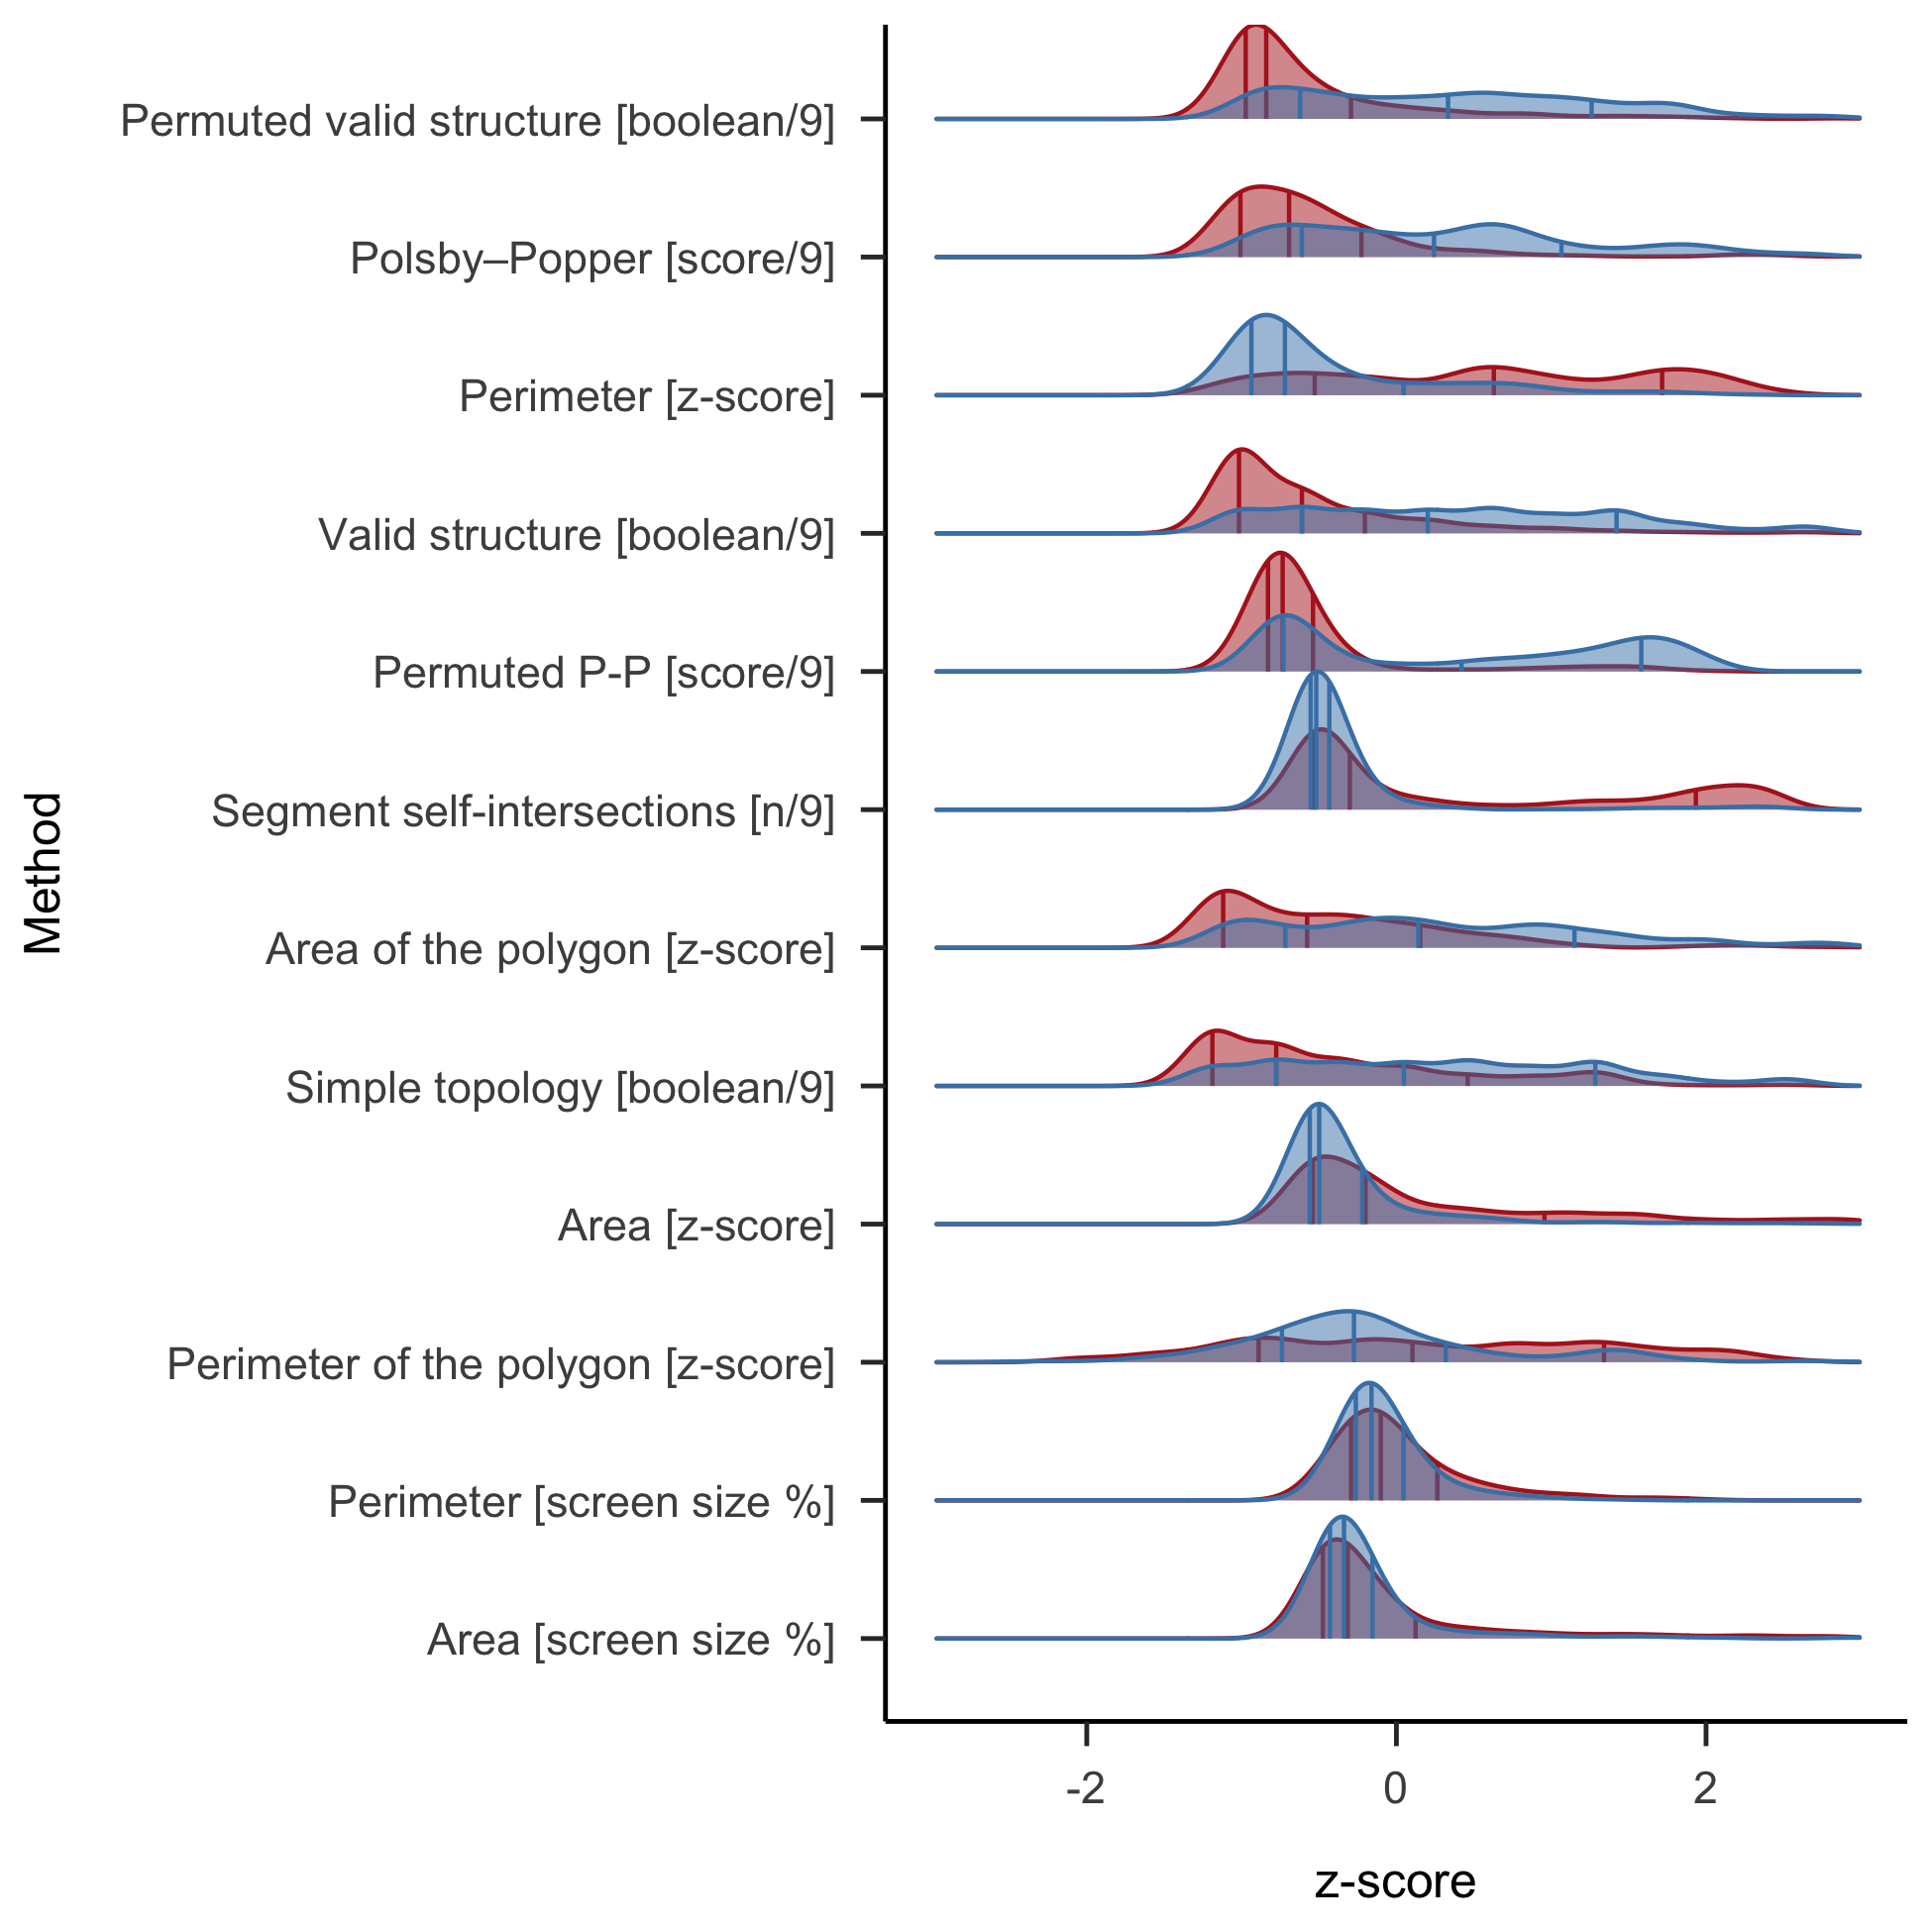
\includegraphics[keepaspectratio]{2.RegisteredReport_MS3_files/figure-pdf/fig-apx01-1.png}}

\vspace{-20pt}
\noindent \emph{Note.} Red~= Classified as Synesthetes, Blue = as
controls.

All method's score have been standardized (\emph{z-score}). x axis
trimmed between -3 and 3 z-scores. Vertical line represent respectively
20, 50 (median) and 80 percentiles of participant's distributions by
self-reported SSS or Control.

\end{figure}

\section{ROC analysis by dataset}\label{apx-SM2byds}

Here we compare the ROC analyses results for each data sample of the
three methods with the best AUC, see Figure~\ref{fig-apx02} and
Table~\ref{tbl-apx02}. Descriptively, we also looked a the distributions
of each methods across SSS and controls Figure~\ref{fig-apx03}. Note
that the dataset labelled as Ward 2 has more synaesthetes than controls
(5:1 ratio). Note that some of the tests led to 100 \% Specificity in
Van Petersen et al. (\citeproc{ref-vanpetersen2020}{2020}) dataset.

\begin{table}

{\caption{{Average feature for Synesthetes by
dataset}{\label{tbl-apx02}}}
\vspace{-20pt}}

\fontsize{12.0pt}{14.0pt}\selectfont
\begin{tabular*}{\linewidth}{@{\extracolsep{\fill}}>{\raggedright\arraybackslash}p{\dimexpr 112.50pt -2\tabcolsep-1.5\arrayrulewidth}rrrrrrrr}
\toprule
 & \multicolumn{4}{c}{{Control}} & \multicolumn{4}{c}{{SSS}} \\ 
\cmidrule(lr){2-5} \cmidrule(lr){6-9}
Feature & PeterCor & Rothen & Ward & Ward2 & PeterCor & Rothen & Ward & Ward2 \\ 
\midrule\addlinespace[2.5pt]
Permuted valid structure [boolean/9] & 0.11 &  0.13 &  0.11 & 0.27 & 0.59 & 0.40 & 0.33 & 0.35 \\ 
Polsby–Popper [score/9] & 0.08 &  0.14 &  0.10 & 0.21 & 0.46 & 0.29 & 0.26 & 0.27 \\ 
Perimeter [z-score] & 1.33 &  2.91 &  3.66 & 2.25 & 0.84 & 1.41 & 1.62 & 1.75 \\ 
Valid structure [boolean/9] & 0.13 &  0.14 &  0.11 & 0.31 & 0.66 & 0.43 & 0.36 & 0.37 \\ 
Permuted P-P [score/9] & 0.06 &  0.11 &  0.10 & 0.33 & 0.61 & 0.40 & 0.40 & 0.41 \\ 
Segment self-intersections [n/9] & 1.41 &  1.78 & 12.26 & 3.02 & 0.22 & 0.26 & 2.23 & 1.85 \\ 
Area of the polygon [z-score] & 0.63 &  1.27 &  0.94 & 1.61 & 2.75 & 2.15 & 1.75 & 2.06 \\ 
Simple topology [boolean/9] & 0.13 &  0.14 &  0.23 & 0.32 & 0.66 & 0.43 & 0.38 & 0.38 \\ 
Area [z-score] & 0.06 &  0.23 &  0.29 & 0.19 & 0.02 & 0.05 & 0.08 & 0.09 \\ 
Perimeter of the polygon [z-score] & 8.87 & 11.21 &  9.27 & 9.21 & 7.98 & 9.06 & 8.29 & 8.50 \\ 
Perimeter [screen size \%] & 0.02 &  0.05 &  0.03 & 0.04 & 0.01 & 0.03 & 0.03 & 0.03 \\ 
Area [screen size \%] & 0.31 &  0.89 &  0.37 & 0.80 & 0.10 & 0.14 & 0.26 & 0.34 \\ 
\bottomrule
\end{tabular*}

\end{table}

\begin{table}

{\caption{{Average zs feature for Synesthetes by
dataset}{\label{tbl-apx02b}}}
\vspace{-20pt}}

\fontsize{12.0pt}{14.0pt}\selectfont
\begin{tabular*}{\linewidth}{@{\extracolsep{\fill}}>{\raggedright\arraybackslash}p{\dimexpr 112.50pt -2\tabcolsep-1.5\arrayrulewidth}rrrrrrrr}
\toprule
 & \multicolumn{4}{c}{{Control}} & \multicolumn{4}{c}{{SSS}} \\ 
\cmidrule(lr){2-5} \cmidrule(lr){6-9}
Feature & PeterCor & Rothen & Ward & Ward2 & PeterCor & Rothen & Ward & Ward2 \\ 
\midrule\addlinespace[2.5pt]
Permuted valid structure [boolean/9] & -0.61 & -0.52 & -0.62 &  0.05 &  1.36 &  0.60 &  0.32 &  0.39 \\ 
Polsby–Popper [score/9] & -0.66 & -0.36 & -0.57 &  0.01 &  1.39 &  0.47 &  0.28 &  0.37 \\ 
Perimeter [z-score] & -0.59 &  0.36 &  0.81 & -0.03 & -0.89 & -0.54 & -0.42 & -0.34 \\ 
Valid structure [boolean/9] & -0.53 & -0.50 & -0.60 &  0.13 &  1.39 &  0.57 &  0.31 &  0.33 \\ 
Permuted P-P [score/9] & -0.73 & -0.58 & -0.59 &  0.13 &  1.04 &  0.38 &  0.35 &  0.40 \\ 
Segment self-intersections [n/9] & -0.40 & -0.36 &  0.78 & -0.23 & -0.53 & -0.53 & -0.31 & -0.35 \\ 
Area of the polygon [z-score] & -0.71 & -0.20 & -0.47 &  0.06 &  0.97 &  0.49 &  0.18 &  0.42 \\ 
Simple topology [boolean/9] & -0.70 & -0.66 & -0.34 &  0.00 &  1.26 &  0.42 &  0.20 &  0.22 \\ 
Area [z-score] & -0.35 &  0.29 &  0.54 &  0.14 & -0.53 & -0.42 & -0.29 & -0.25 \\ 
Perimeter of the polygon [z-score] &  0.01 &  0.79 &  0.14 &  0.12 & -0.29 &  0.07 & -0.19 & -0.12 \\ 
Perimeter [screen size \%] & -0.13 &  0.32 & -0.02 &  0.19 & -0.27 & -0.08 &  0.01 & -0.03 \\ 
Area [screen size \%] & -0.04 &  0.79 &  0.04 &  0.65 & -0.35 & -0.29 & -0.12 &  0.00 \\ 
\bottomrule
\end{tabular*}

\end{table}

\begin{figure}

{\caption{{Lineplots of AUC and DP by data source}{\label{fig-apx02}}}}

\pandocbounded{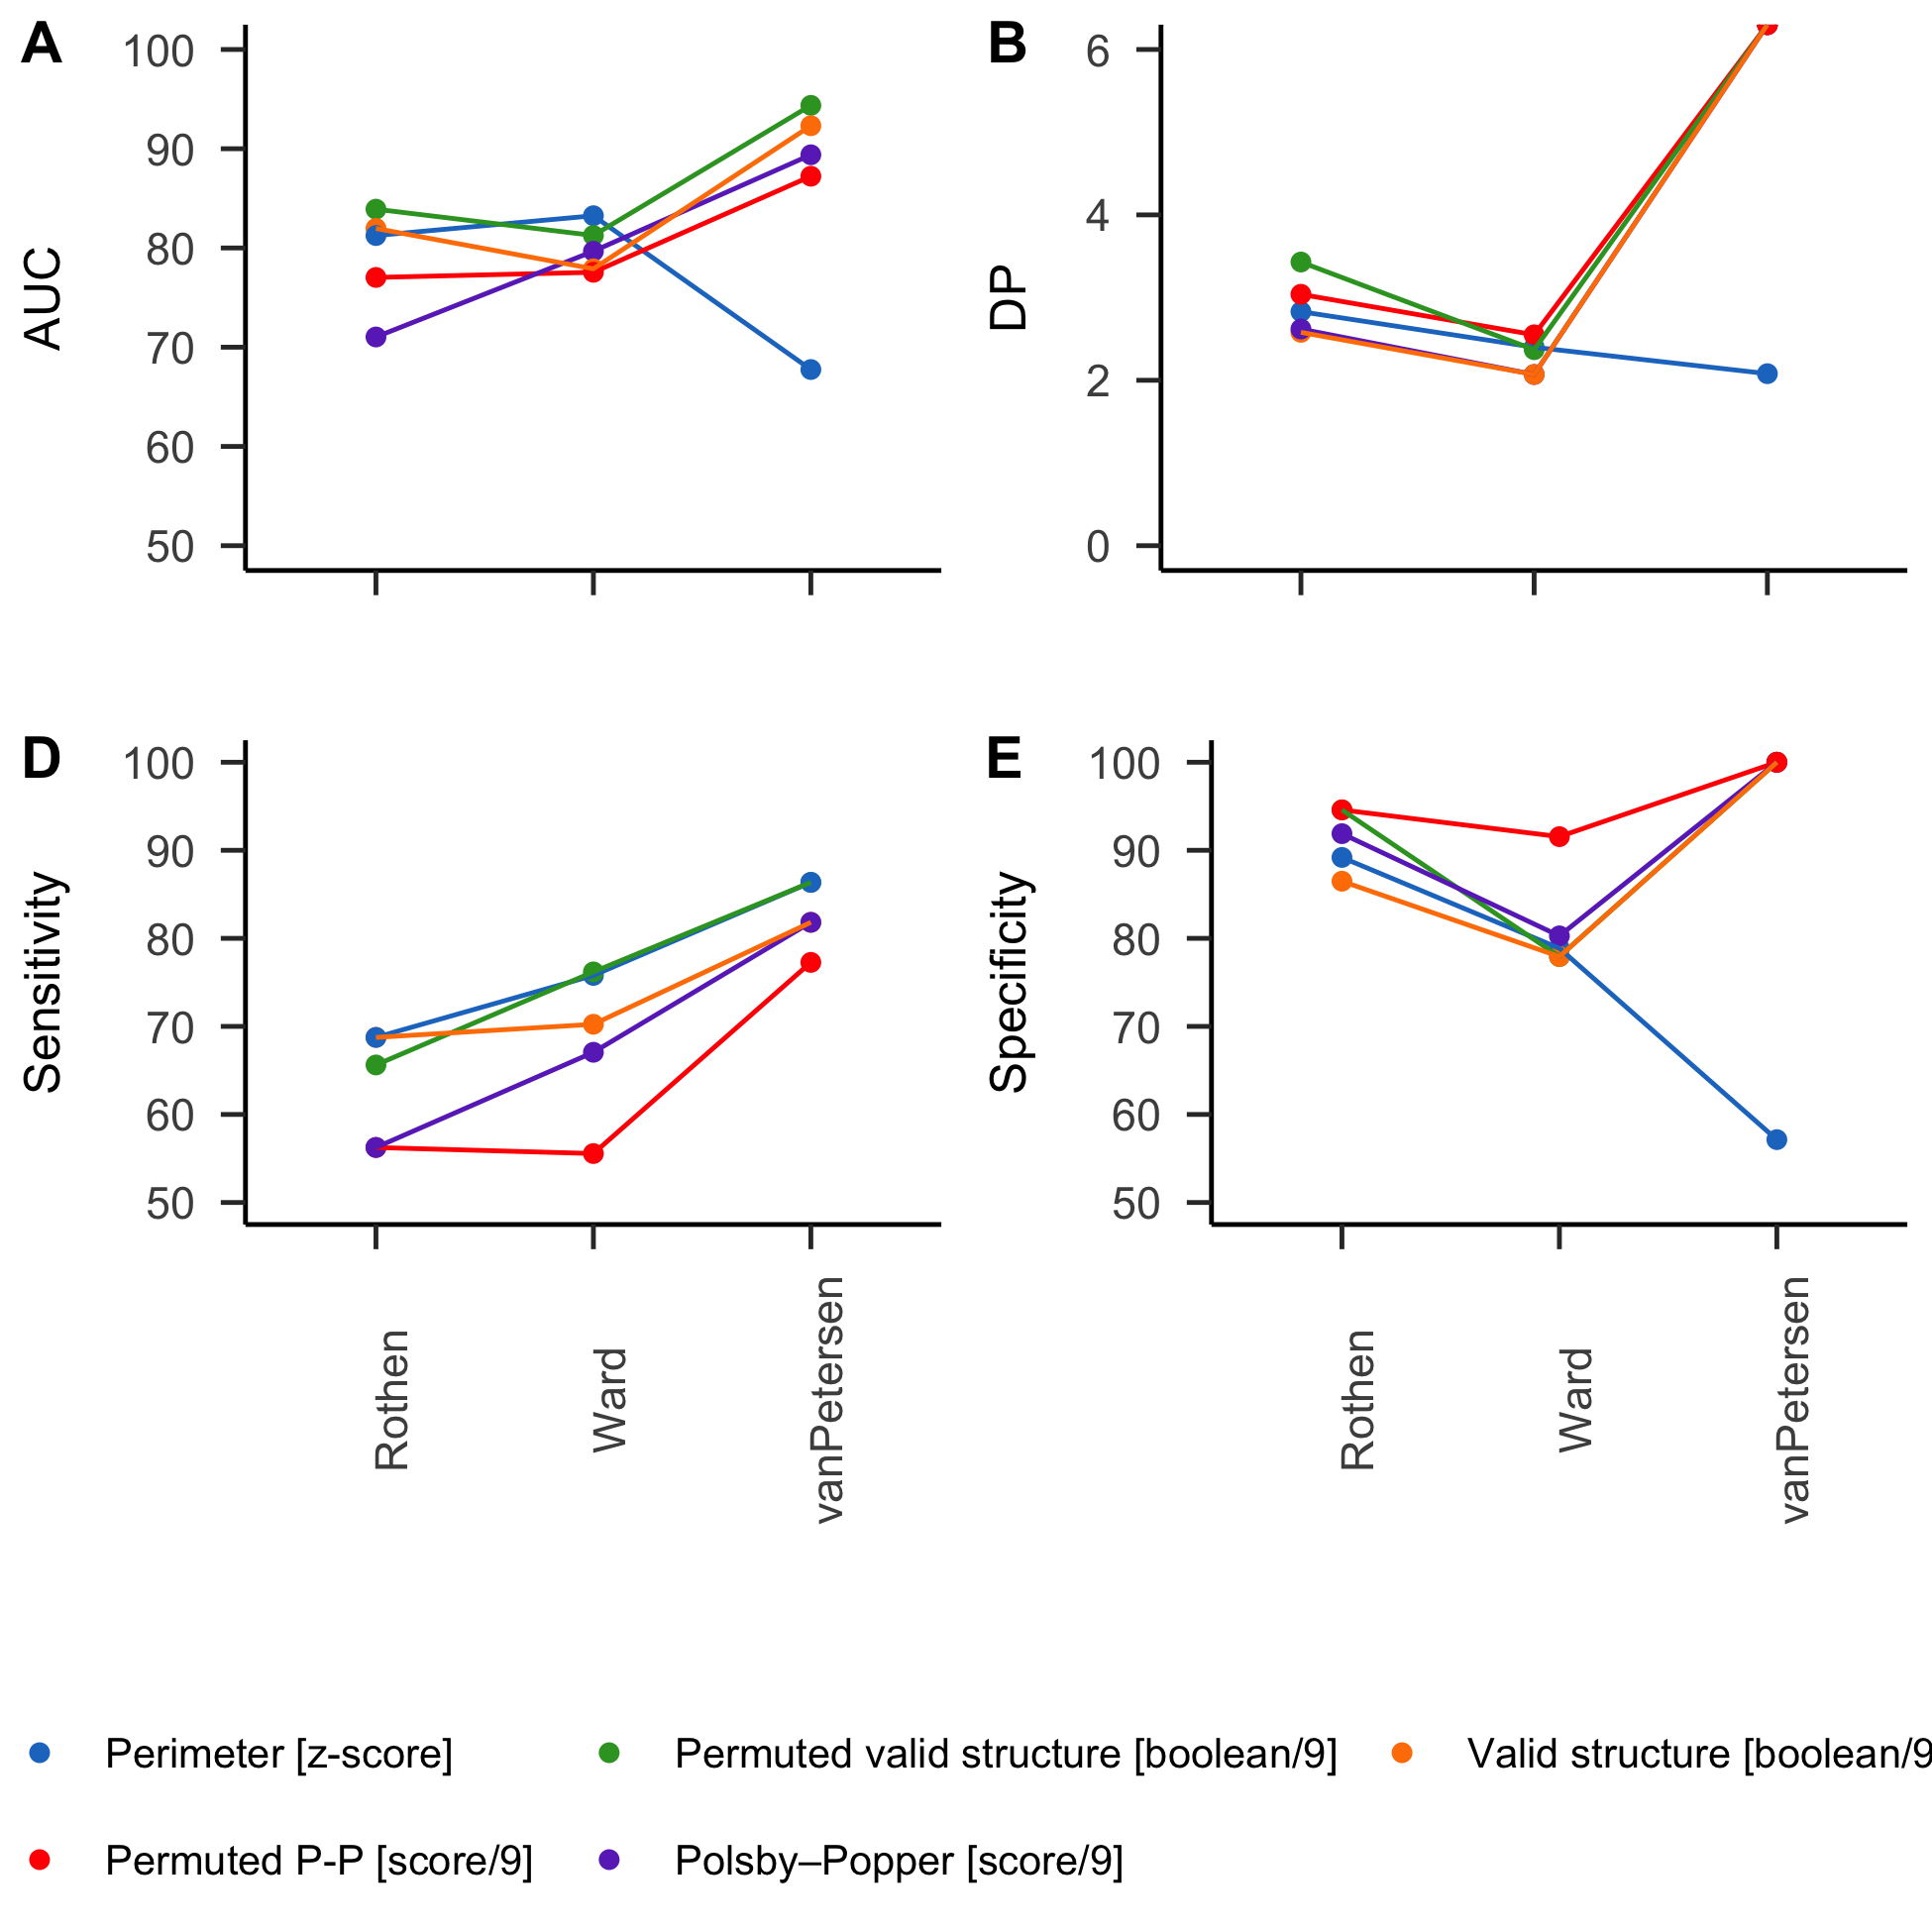
\includegraphics[keepaspectratio]{2.RegisteredReport_MS3_files/figure-pdf/fig-apx02-1.png}}

\vspace{-20pt}
\noindent \emph{Note.} AUC~= Area Under the Curve, DP = Discrimination
Power

\end{figure}

\begin{figure}

{\caption{{Density plots of all the consistency tests comparing SSS and
controls by dataset}{\label{fig-apx03}}}}

\pandocbounded{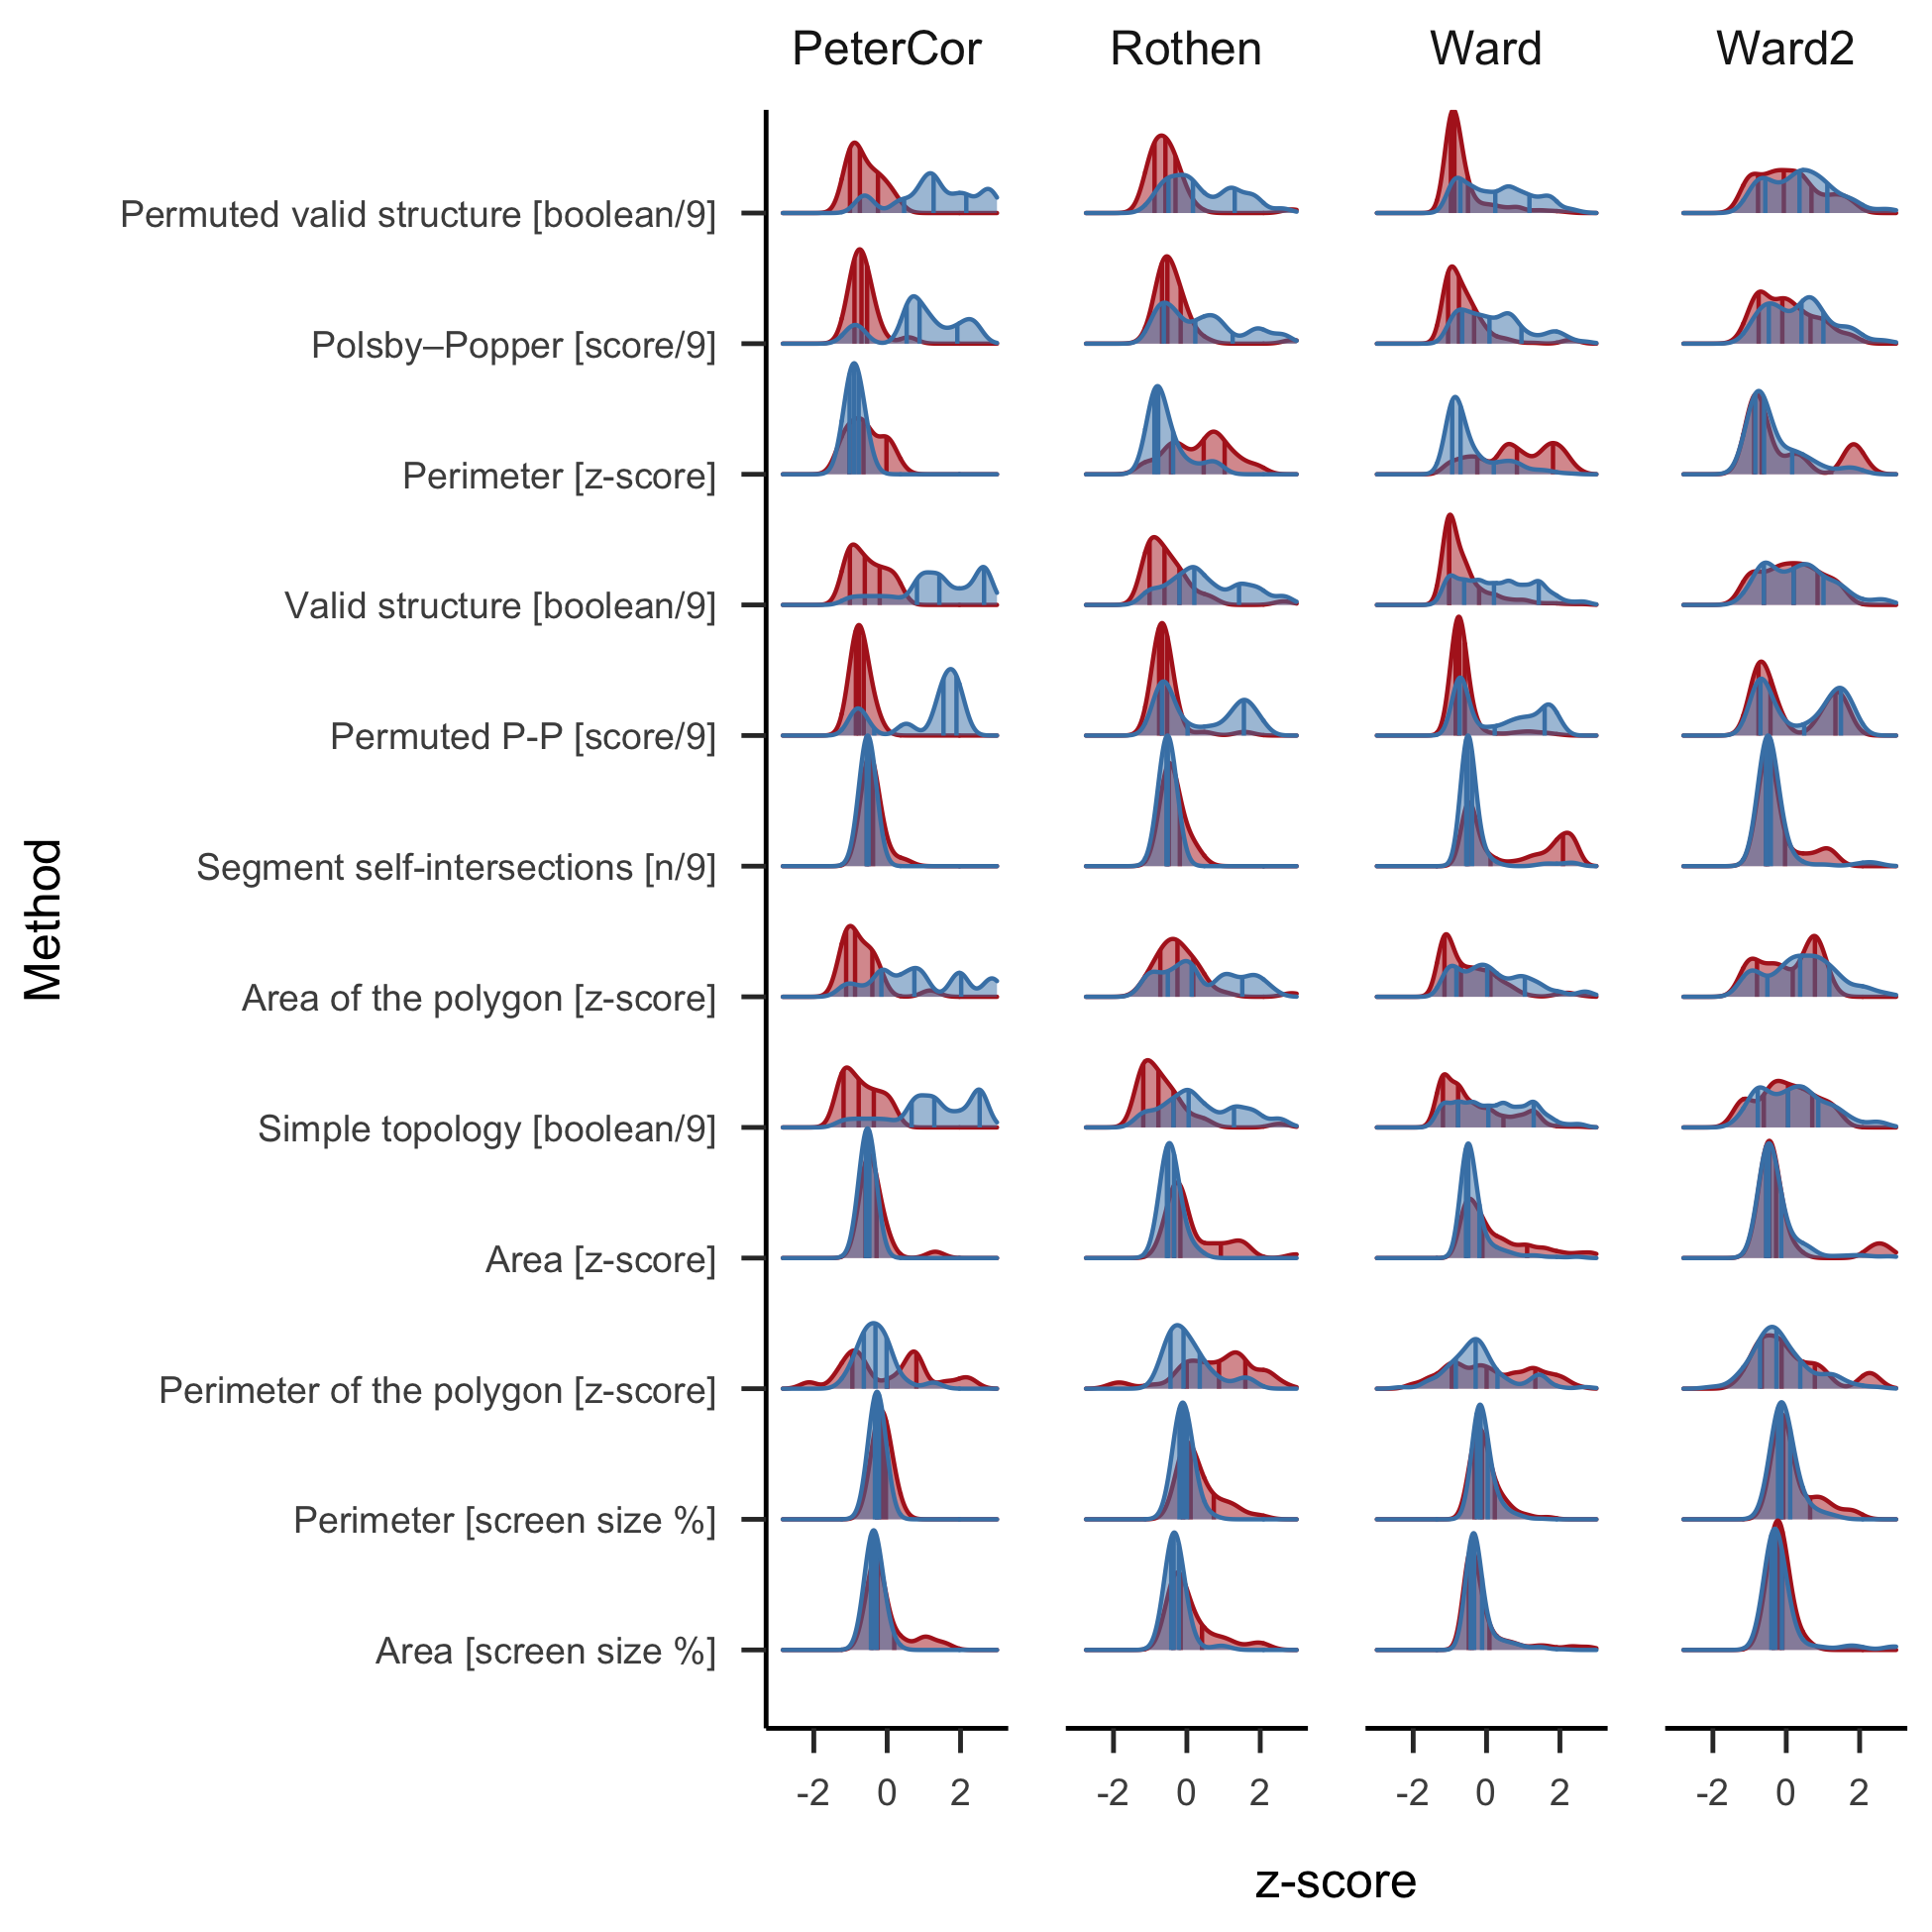
\includegraphics[keepaspectratio]{2.RegisteredReport_MS3_files/figure-pdf/fig-apx03-1.png}}

\vspace{-20pt}
\noindent \emph{Note.} Red~= Classified as Synesthetes, Blue = as
controls.

All method's score have been standardized (\emph{z-score}). x axis
trimmed between -3 and 3 z-scores. Vertical line indicate respectively
20, 50 (median) and 80 percentiles of each distributions.

\end{figure}

\section{ROC Analysis Sub-sampled data by questionnaire quantiles (20\%
steps)}\label{apx-byquestperc}

We compared the data sampled by the questionnaire score. Based on the
distribution of the questionnaire score, we sampled the 10 \% with the
lowest and 10 \% with the highest scores. Those are then compared with
the 20 and 20 \% and so on until 40 and 40 \%. The rationale of this
procedure is that AUC, sensitivity and specificity should remain stable
across percentiles for a feature to be valid, see
Figure~\ref{fig-apx04}. In other words the ROC should remain unchanged
if we take extreme groups compared to less extreme ones.

\begin{figure}

{\caption{{Lineplots of AUC and DP by questionnaire
percentile}{\label{fig-apx04}}}}

\pandocbounded{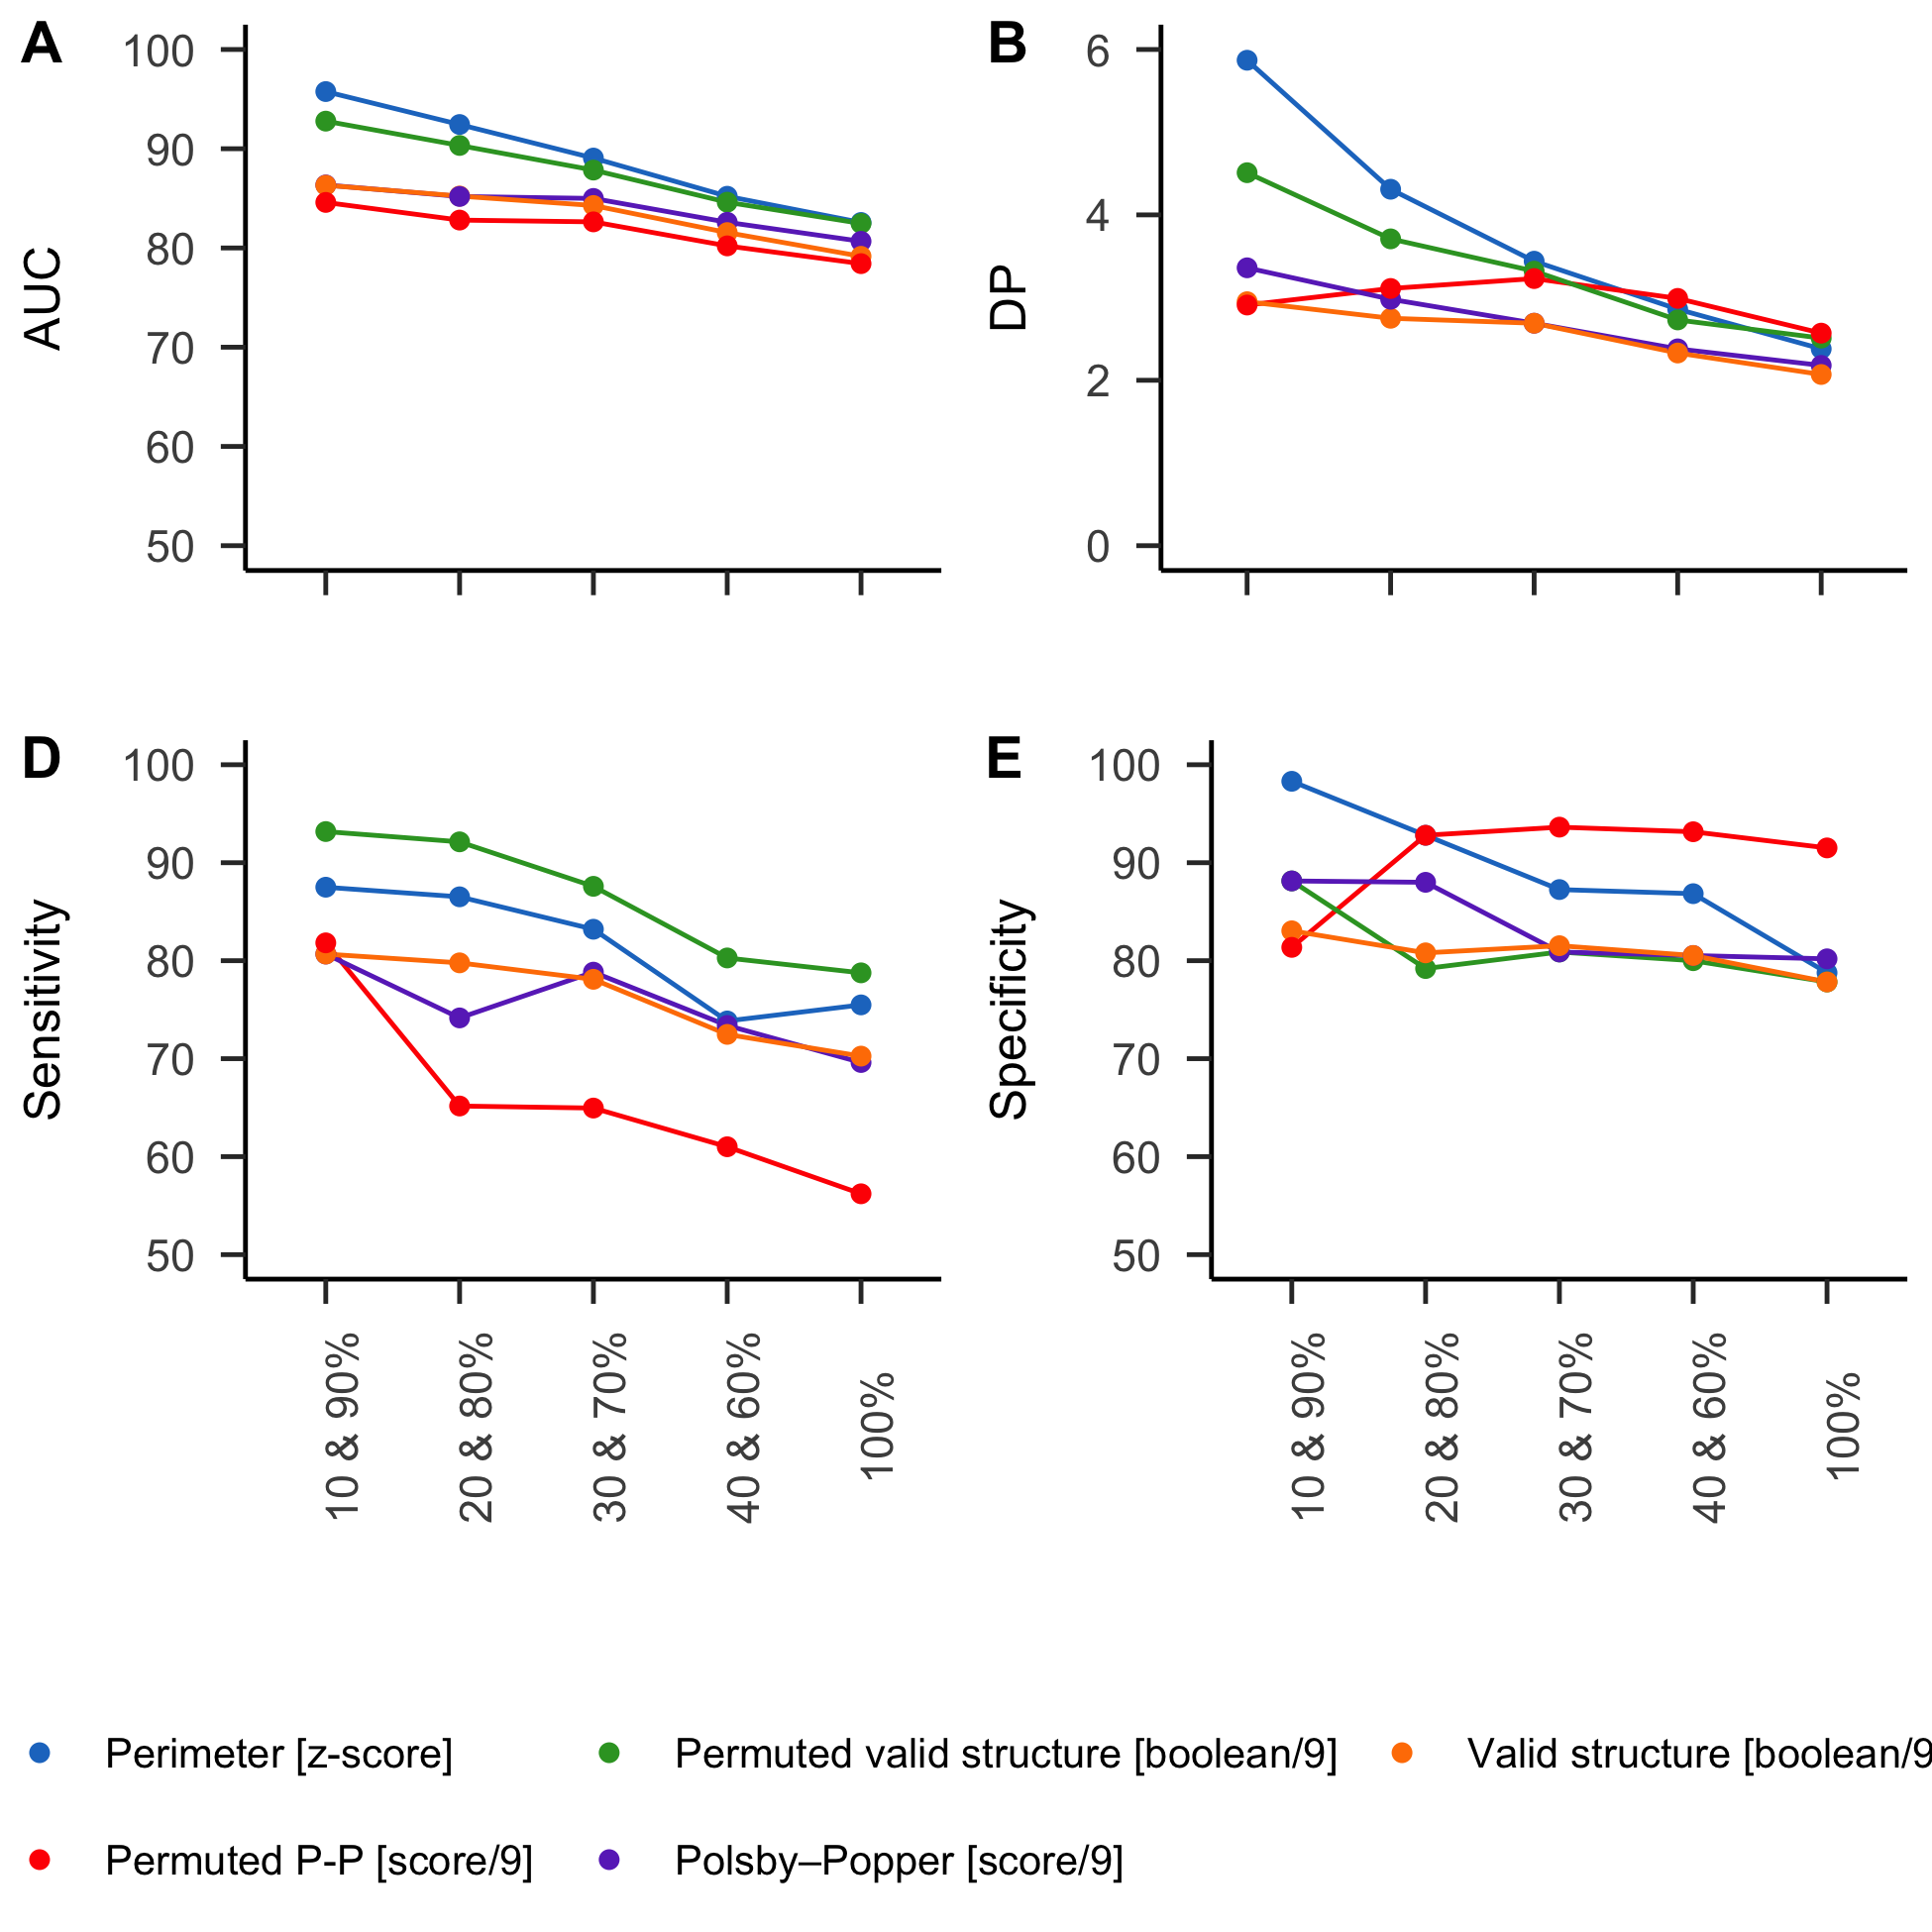
\includegraphics[keepaspectratio]{2.RegisteredReport_MS3_files/figure-pdf/fig-apx04-1.png}}

\vspace{-20pt}
\noindent \emph{Note.} Each~point is an increasing percentiles. AUC =
Area Under the Curve. DP = Discrimination Power. Specitficites of some
tests with van Petersen data are 100\%, so the DP are nor computable nor
interpretable

\end{figure}

\section{Correlation with
self-report}\label{apx-correlation-with-self-report}

The best criterion should also best correlate with SSS self-reported
questionnaire score. Works only with Ward's aggregated data, see
Figure~\ref{fig-apx05}.

\begin{figure}

{\caption{{Correlation with self-reported
questionnaire}{\label{fig-apx05}}}}

\pandocbounded{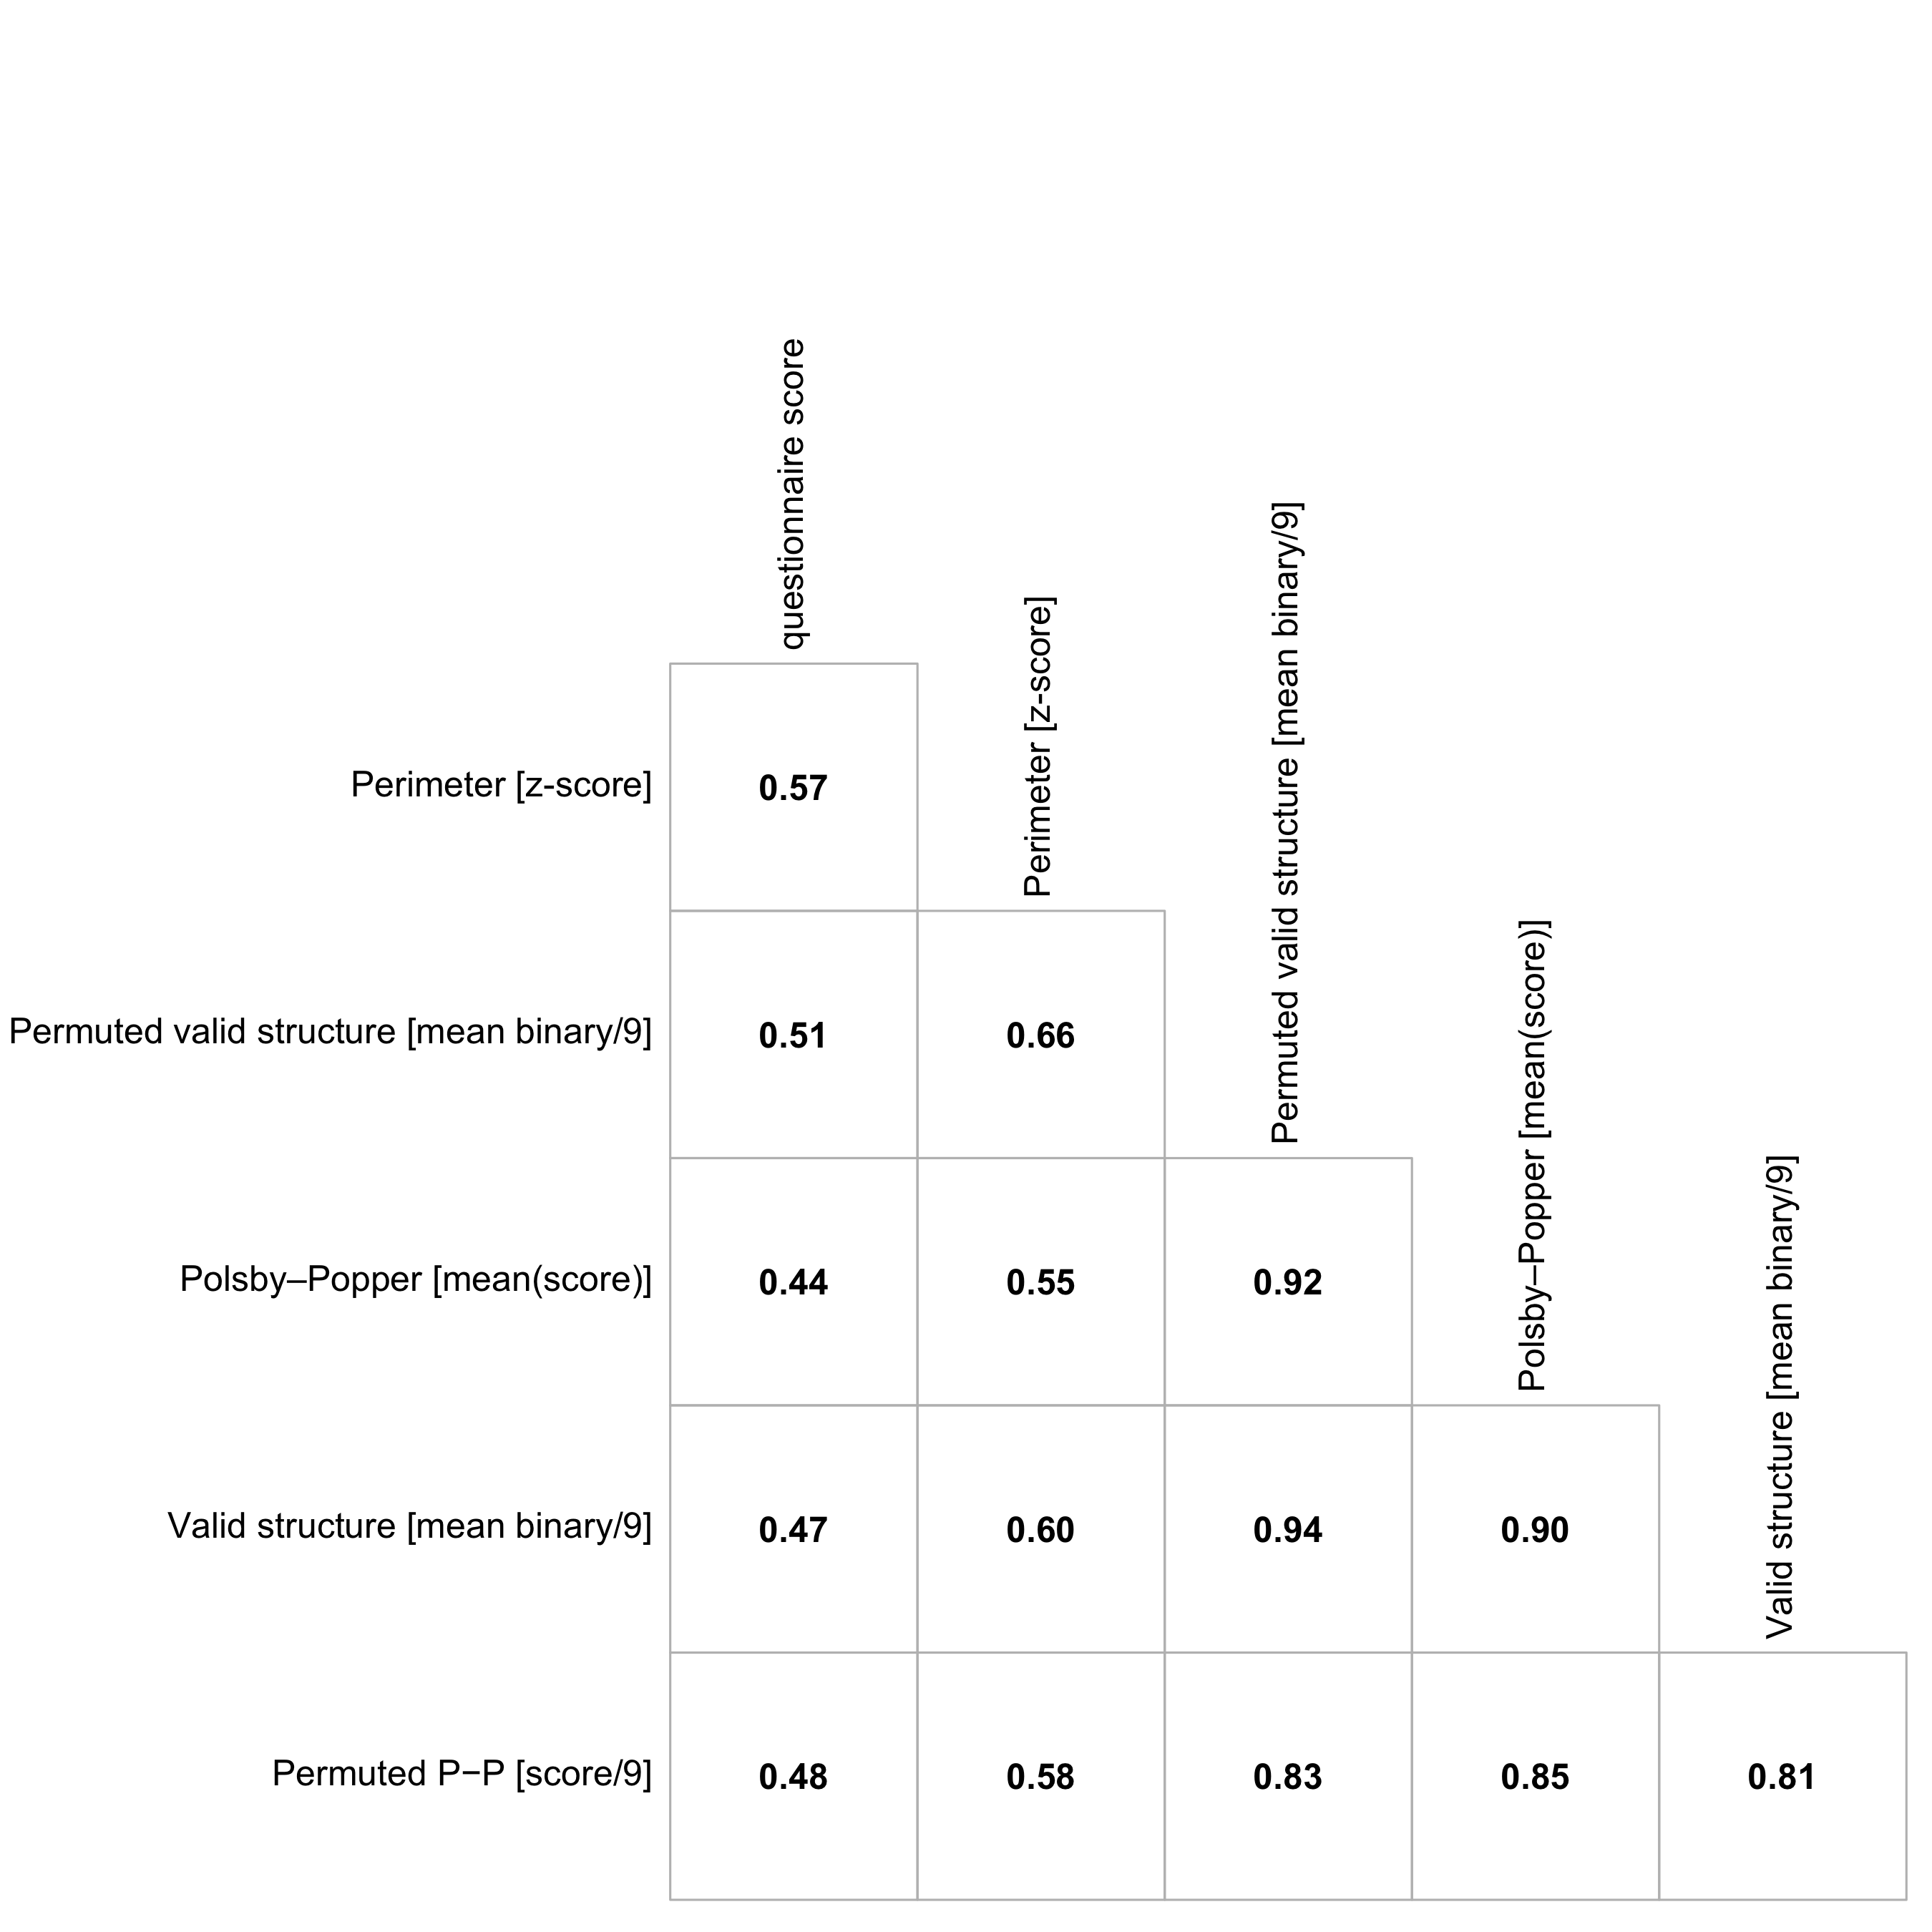
\includegraphics[keepaspectratio]{2.RegisteredReport_MS3_files/figure-pdf/fig-apx05-1.png}}

\vspace{-20pt}
\noindent \emph{Note.} Only~data from Ward is included hereh

\end{figure}

\section{Centred average forms}\label{apx-average-forms}

In this additional analyses we attempted at visualizing the average for
each categories to see whether a pattern could be discerned on a
qualitative level. To avoid negative coordinates, we shifted all the
z-scores from the whole dataset minimum for the x and y coordinates.
Then we anchored to the coordinate 0,0 the stimulus ``1'' for numbers,
``Monday'' for weekdays and ``January'' for months. We then plotted all
the space forms with transparency, see Figure~\ref{fig-apx06}.

Descriptively it is possible to see more circular pattern for months and
horizontal and vertical patterns for numbers. Also the averaged forms
appear to be more clearly defined in the synaesthetes than control.

\begin{figure}

\caption{\label{fig-apx06}Average Centered space forms visualized}

\centering{

\pandocbounded{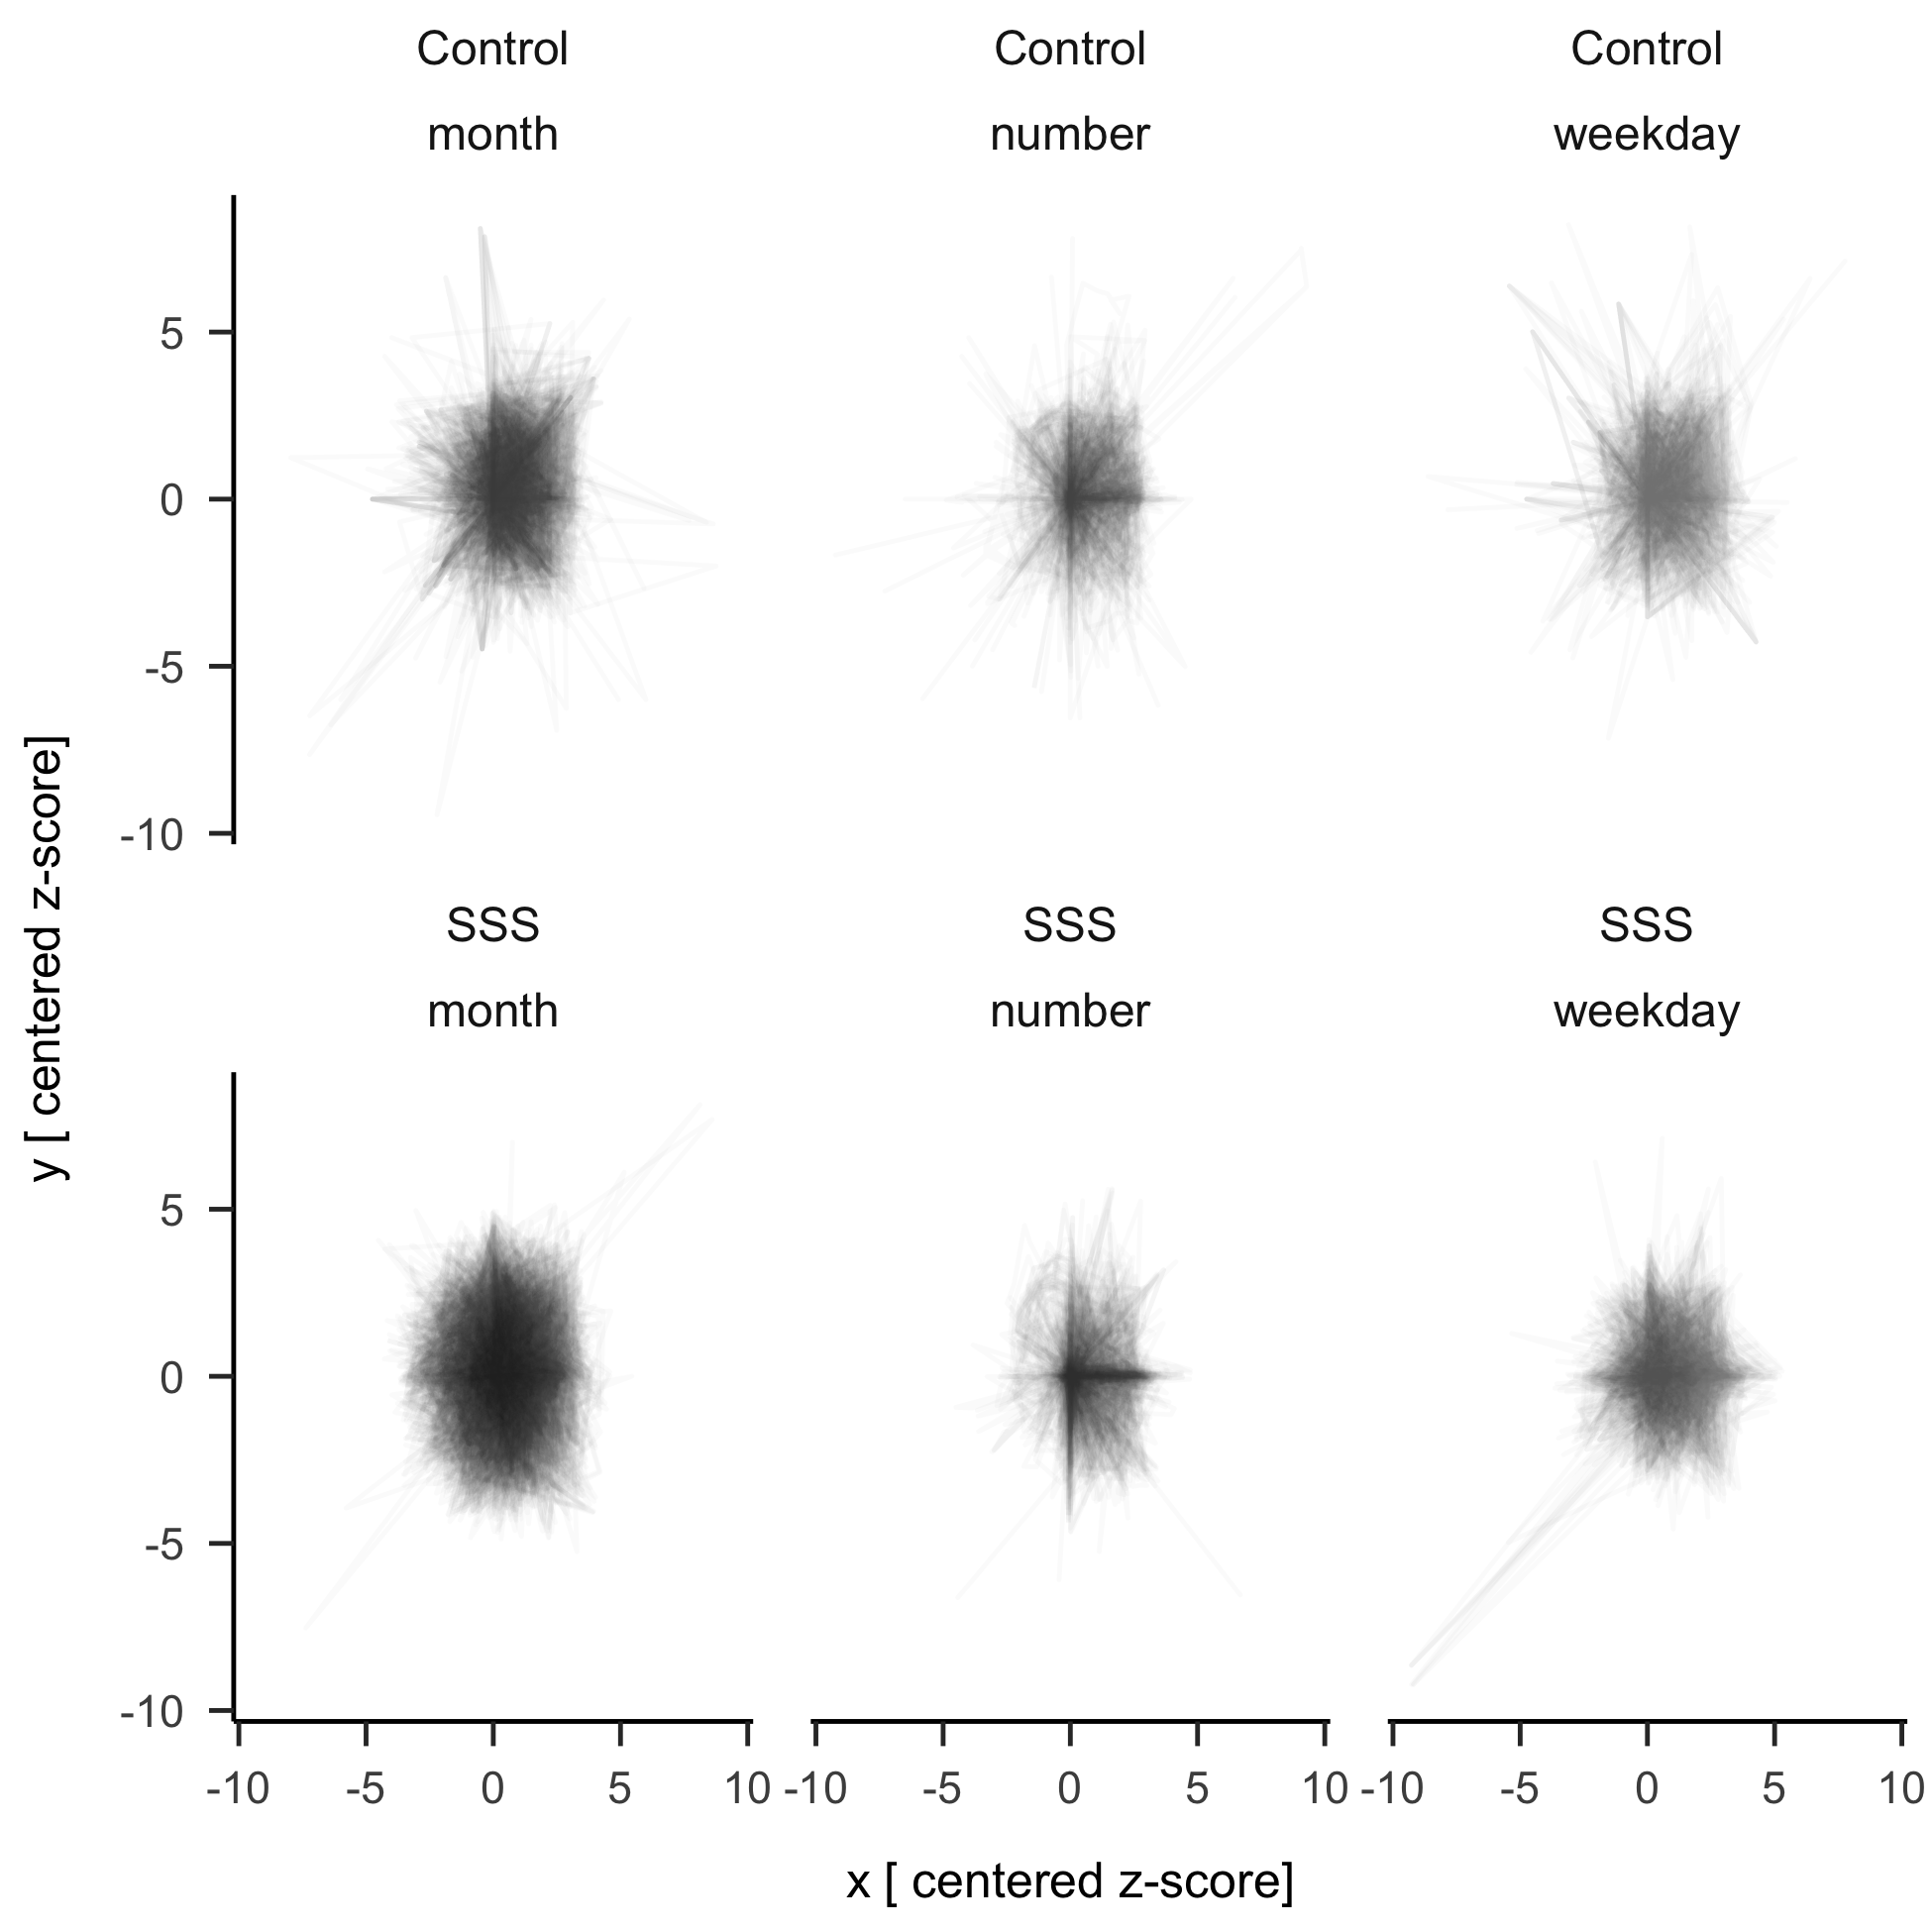
\includegraphics[keepaspectratio]{2.RegisteredReport_MS3_files/figure-pdf/fig-apx06-1.png}}

}

\end{figure}%

\section{Alluvial plot}\label{apx-alluvial}

Are false positives and negatives share some characteristics? To answer
this question qualitatively we identified two group of self-reported SSS
participants who care consistently classified as controls by the five
methods with the highest AUC (i.e.~consistent false negatives), see dark
blue lines in Figure~\ref{fig-apx07}. On the other side we identified a
group of controls who are consistently classified as SSS by the five
methods with the highest AUC, see dark red lines in
Figure~\ref{fig-apx07}.

\begin{figure}

{\caption{{Alluvial plot of test passing}{\label{fig-apx07}}}}

\pandocbounded{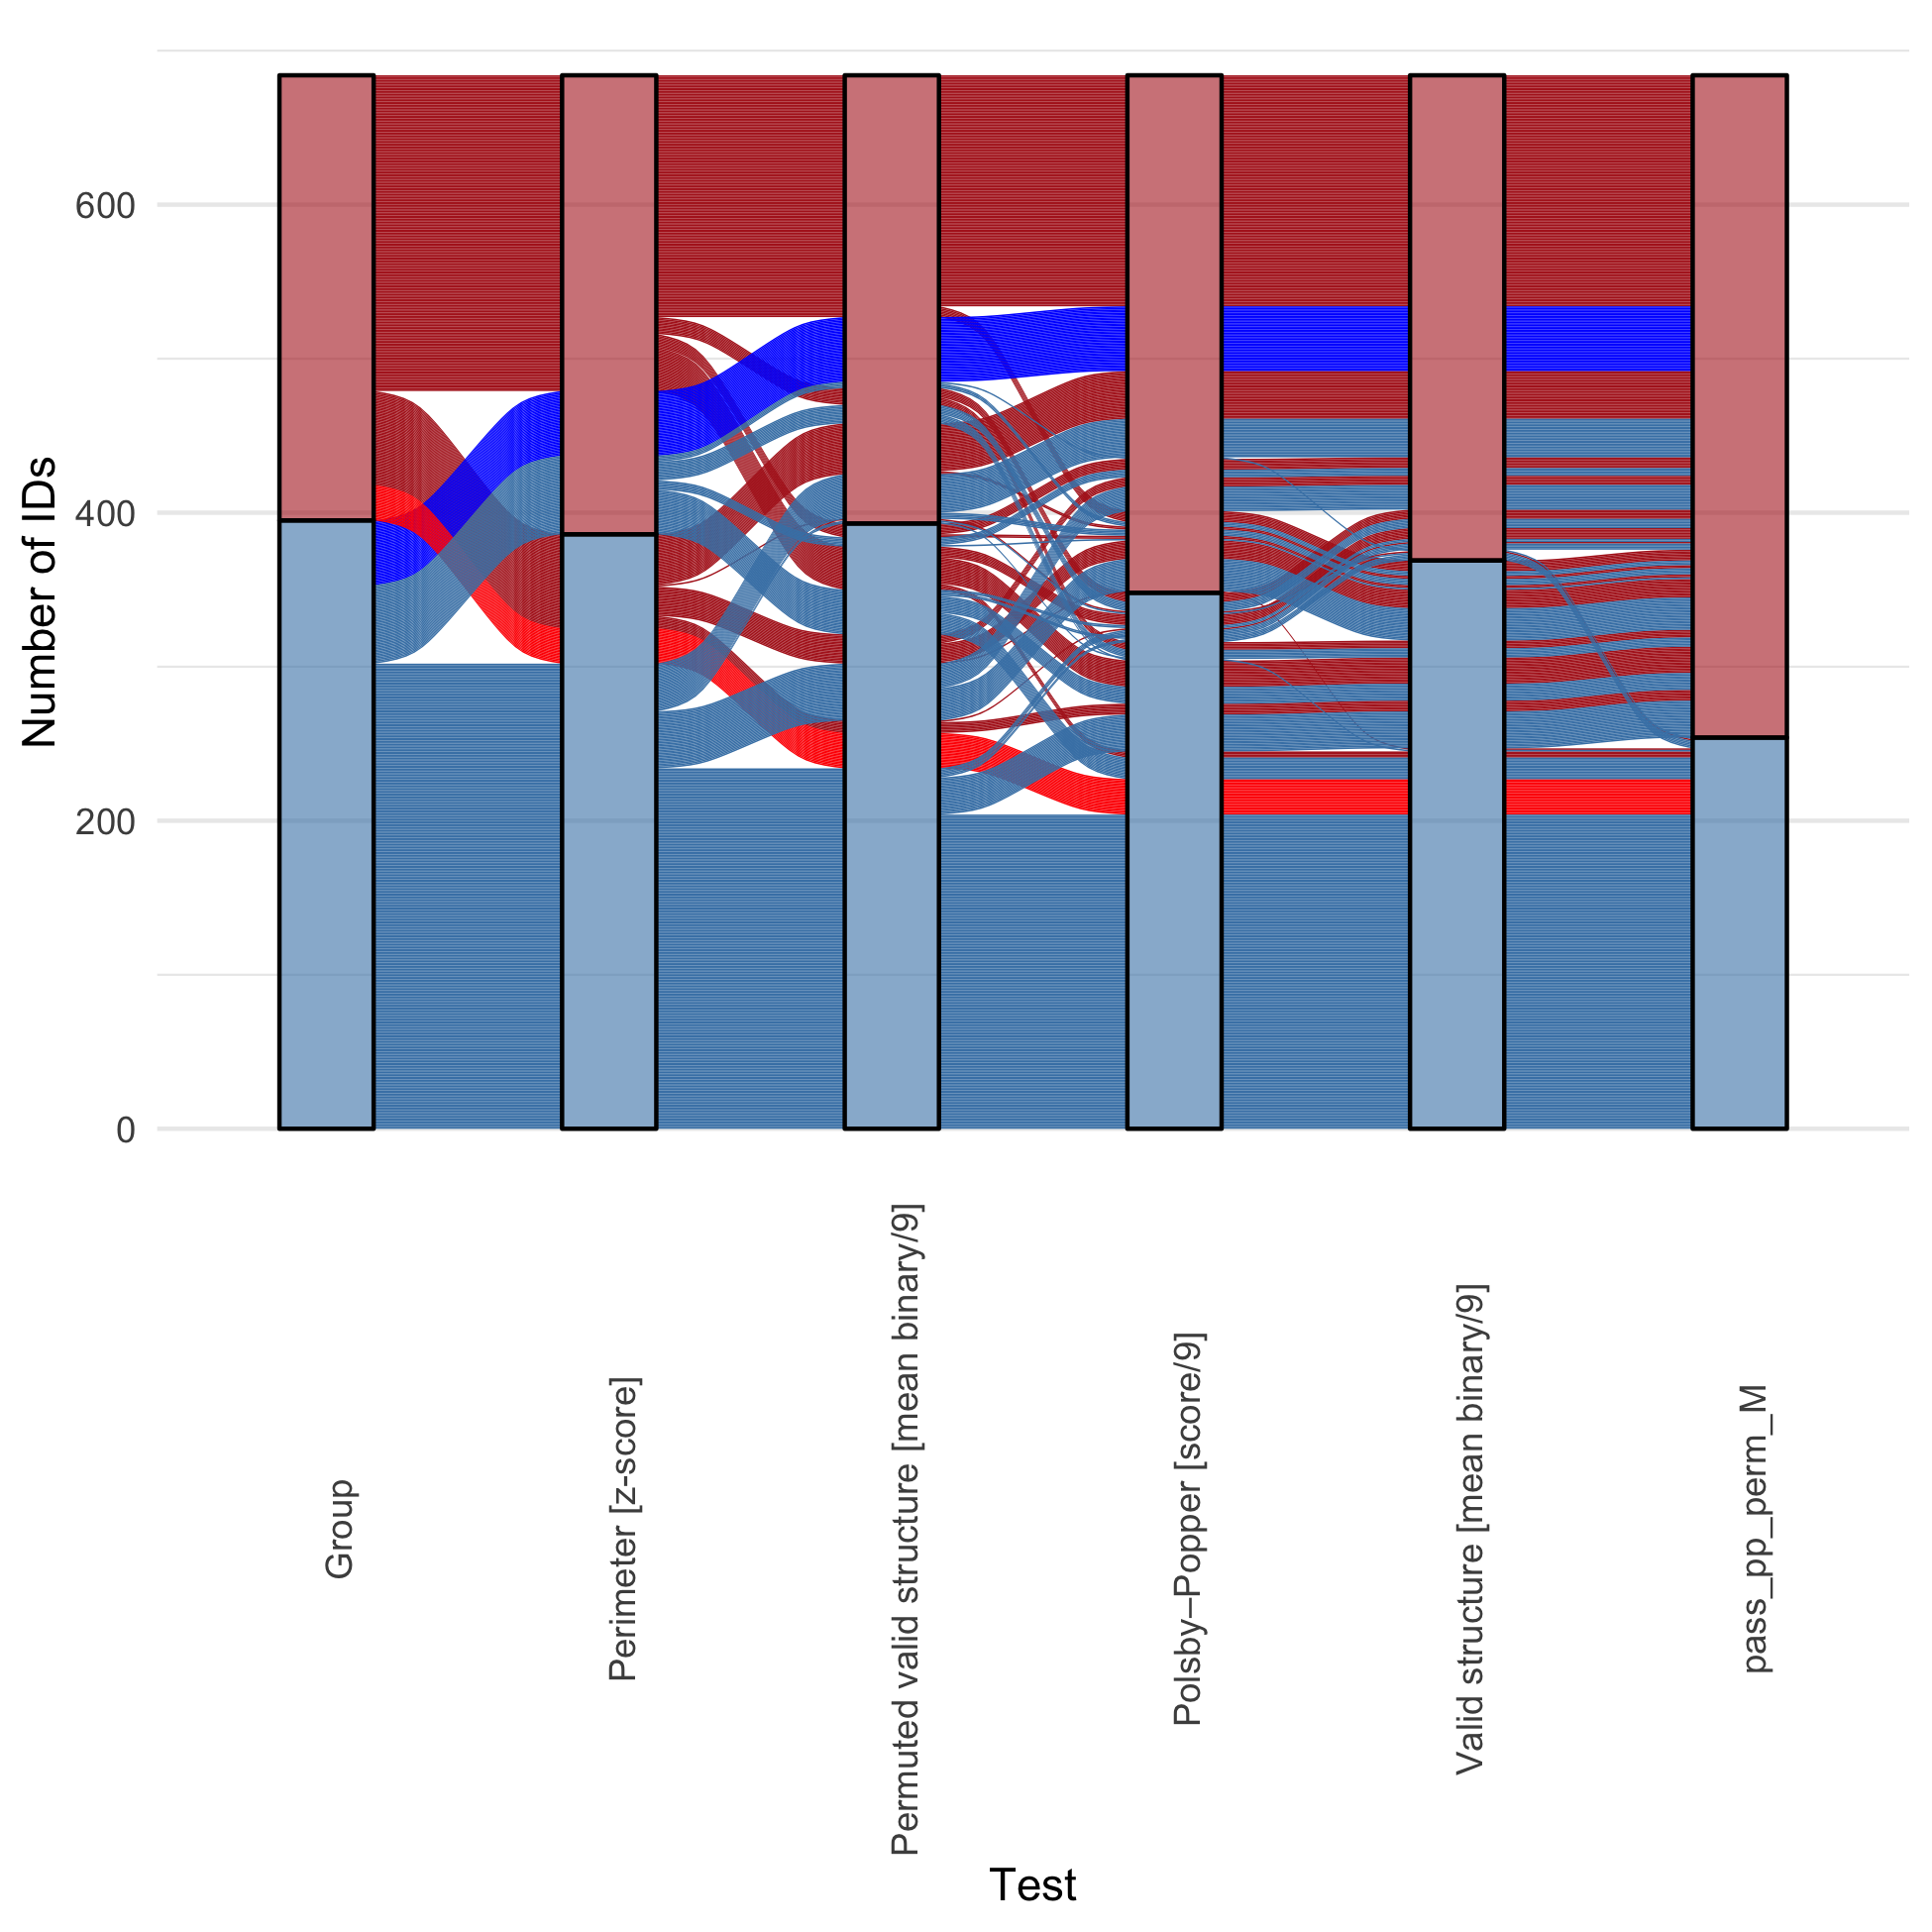
\includegraphics[keepaspectratio]{2.RegisteredReport_MS3_files/figure-pdf/fig-apx07-1.png}}

\vspace{-20pt}
\noindent \emph{Note.} Blue~= Synaesthetes, Red = Controls. Each line
represents a participants classification in SSS or control by each test
at the given threshold. Blue highligh are Synesthetes who are
systematically classified as control by all 5 tests. Red highlight are
controls who are systematically classified as synesthetes by all 5
tests.

\end{figure}

On one side 6.12 \% of all participants, that is 42 Synaesthetes where
consistently classified as controls by all five tests, see
Figure~\ref{fig-apx08}. On the other side 3.35 \% of all participants,
23 controls where consistently classified as SSS by all five tests, see
Figure~\ref{fig-apx09}. Given the different approaches of each methods,
the identified participants might be on one side non-genuine synesthetes
and on the other controls who have SSS but are either not aware or did
not identify it as such.

\begin{figure}

\caption{\label{fig-apx08}Synaesthetes who consistently \emph{fail} all
five tests (blue in the alluvial plot)}

\centering{

\pandocbounded{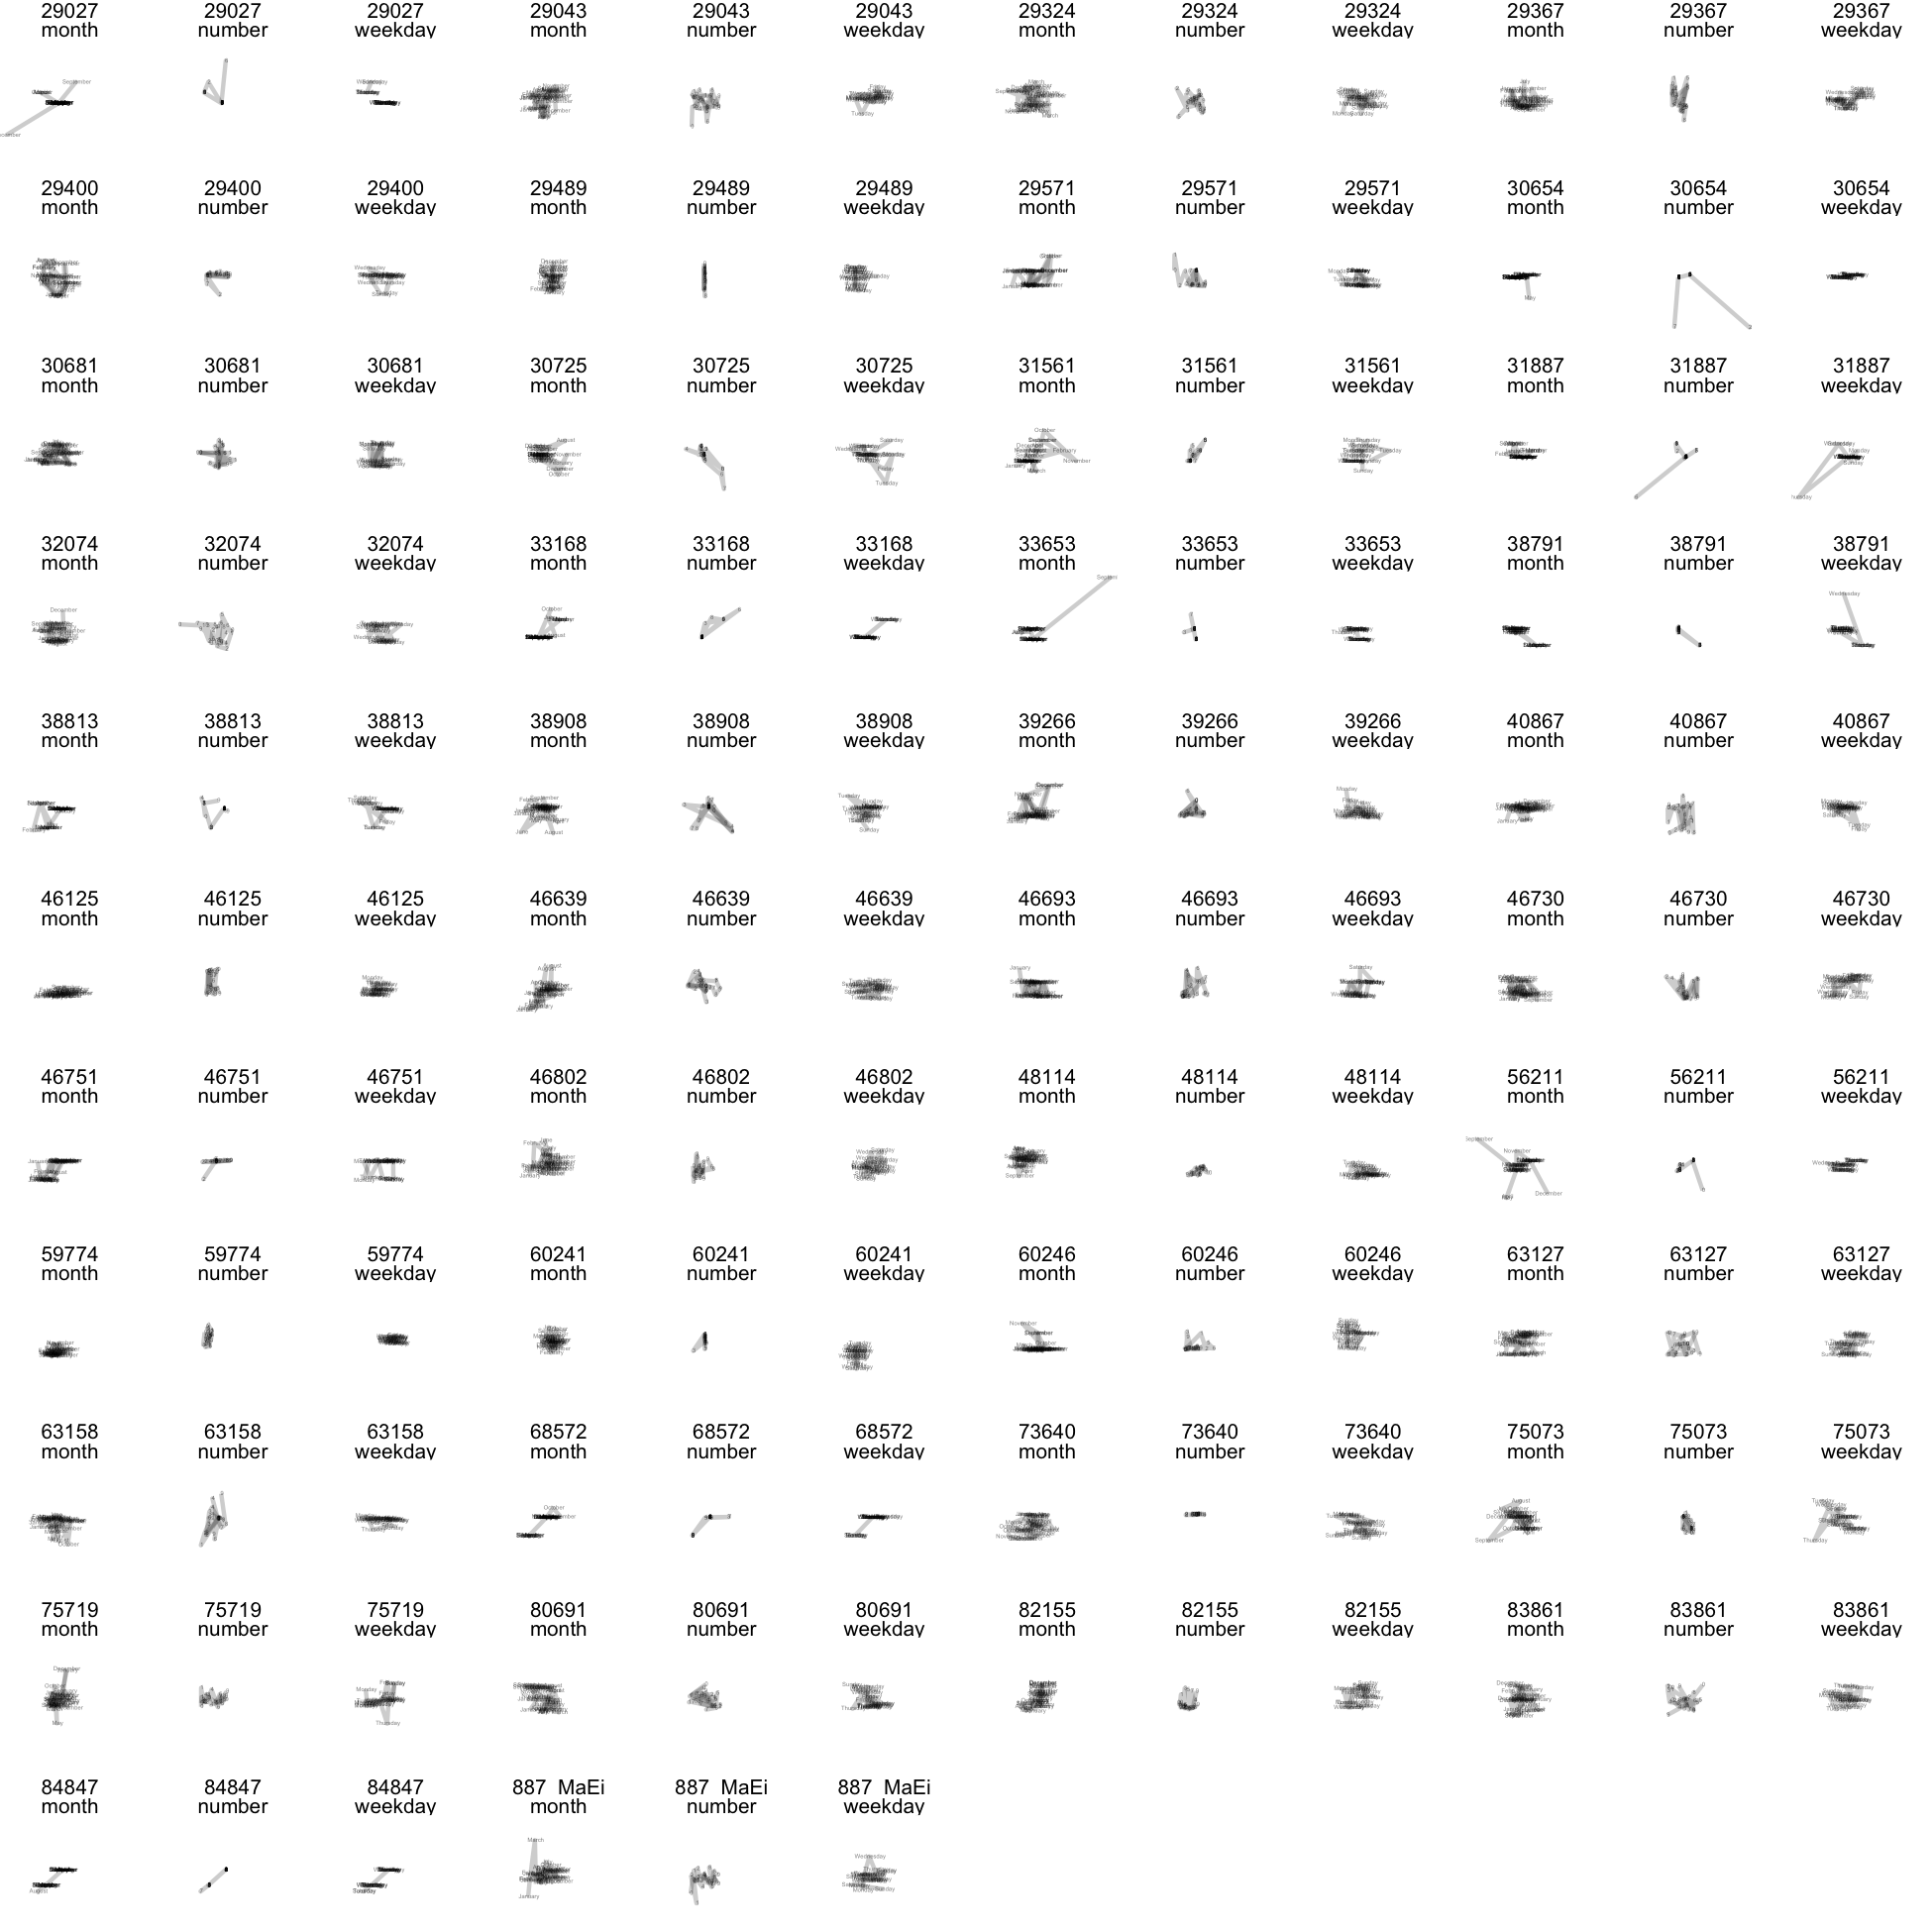
\includegraphics[keepaspectratio]{2.RegisteredReport_MS3_files/figure-pdf/fig-apx08-1.png}}

}

\end{figure}%

\begin{figure}

\caption{\label{fig-apx09}Controls who consistently \emph{pass} all five
tests (red in the alluvial plot)}

\centering{

\pandocbounded{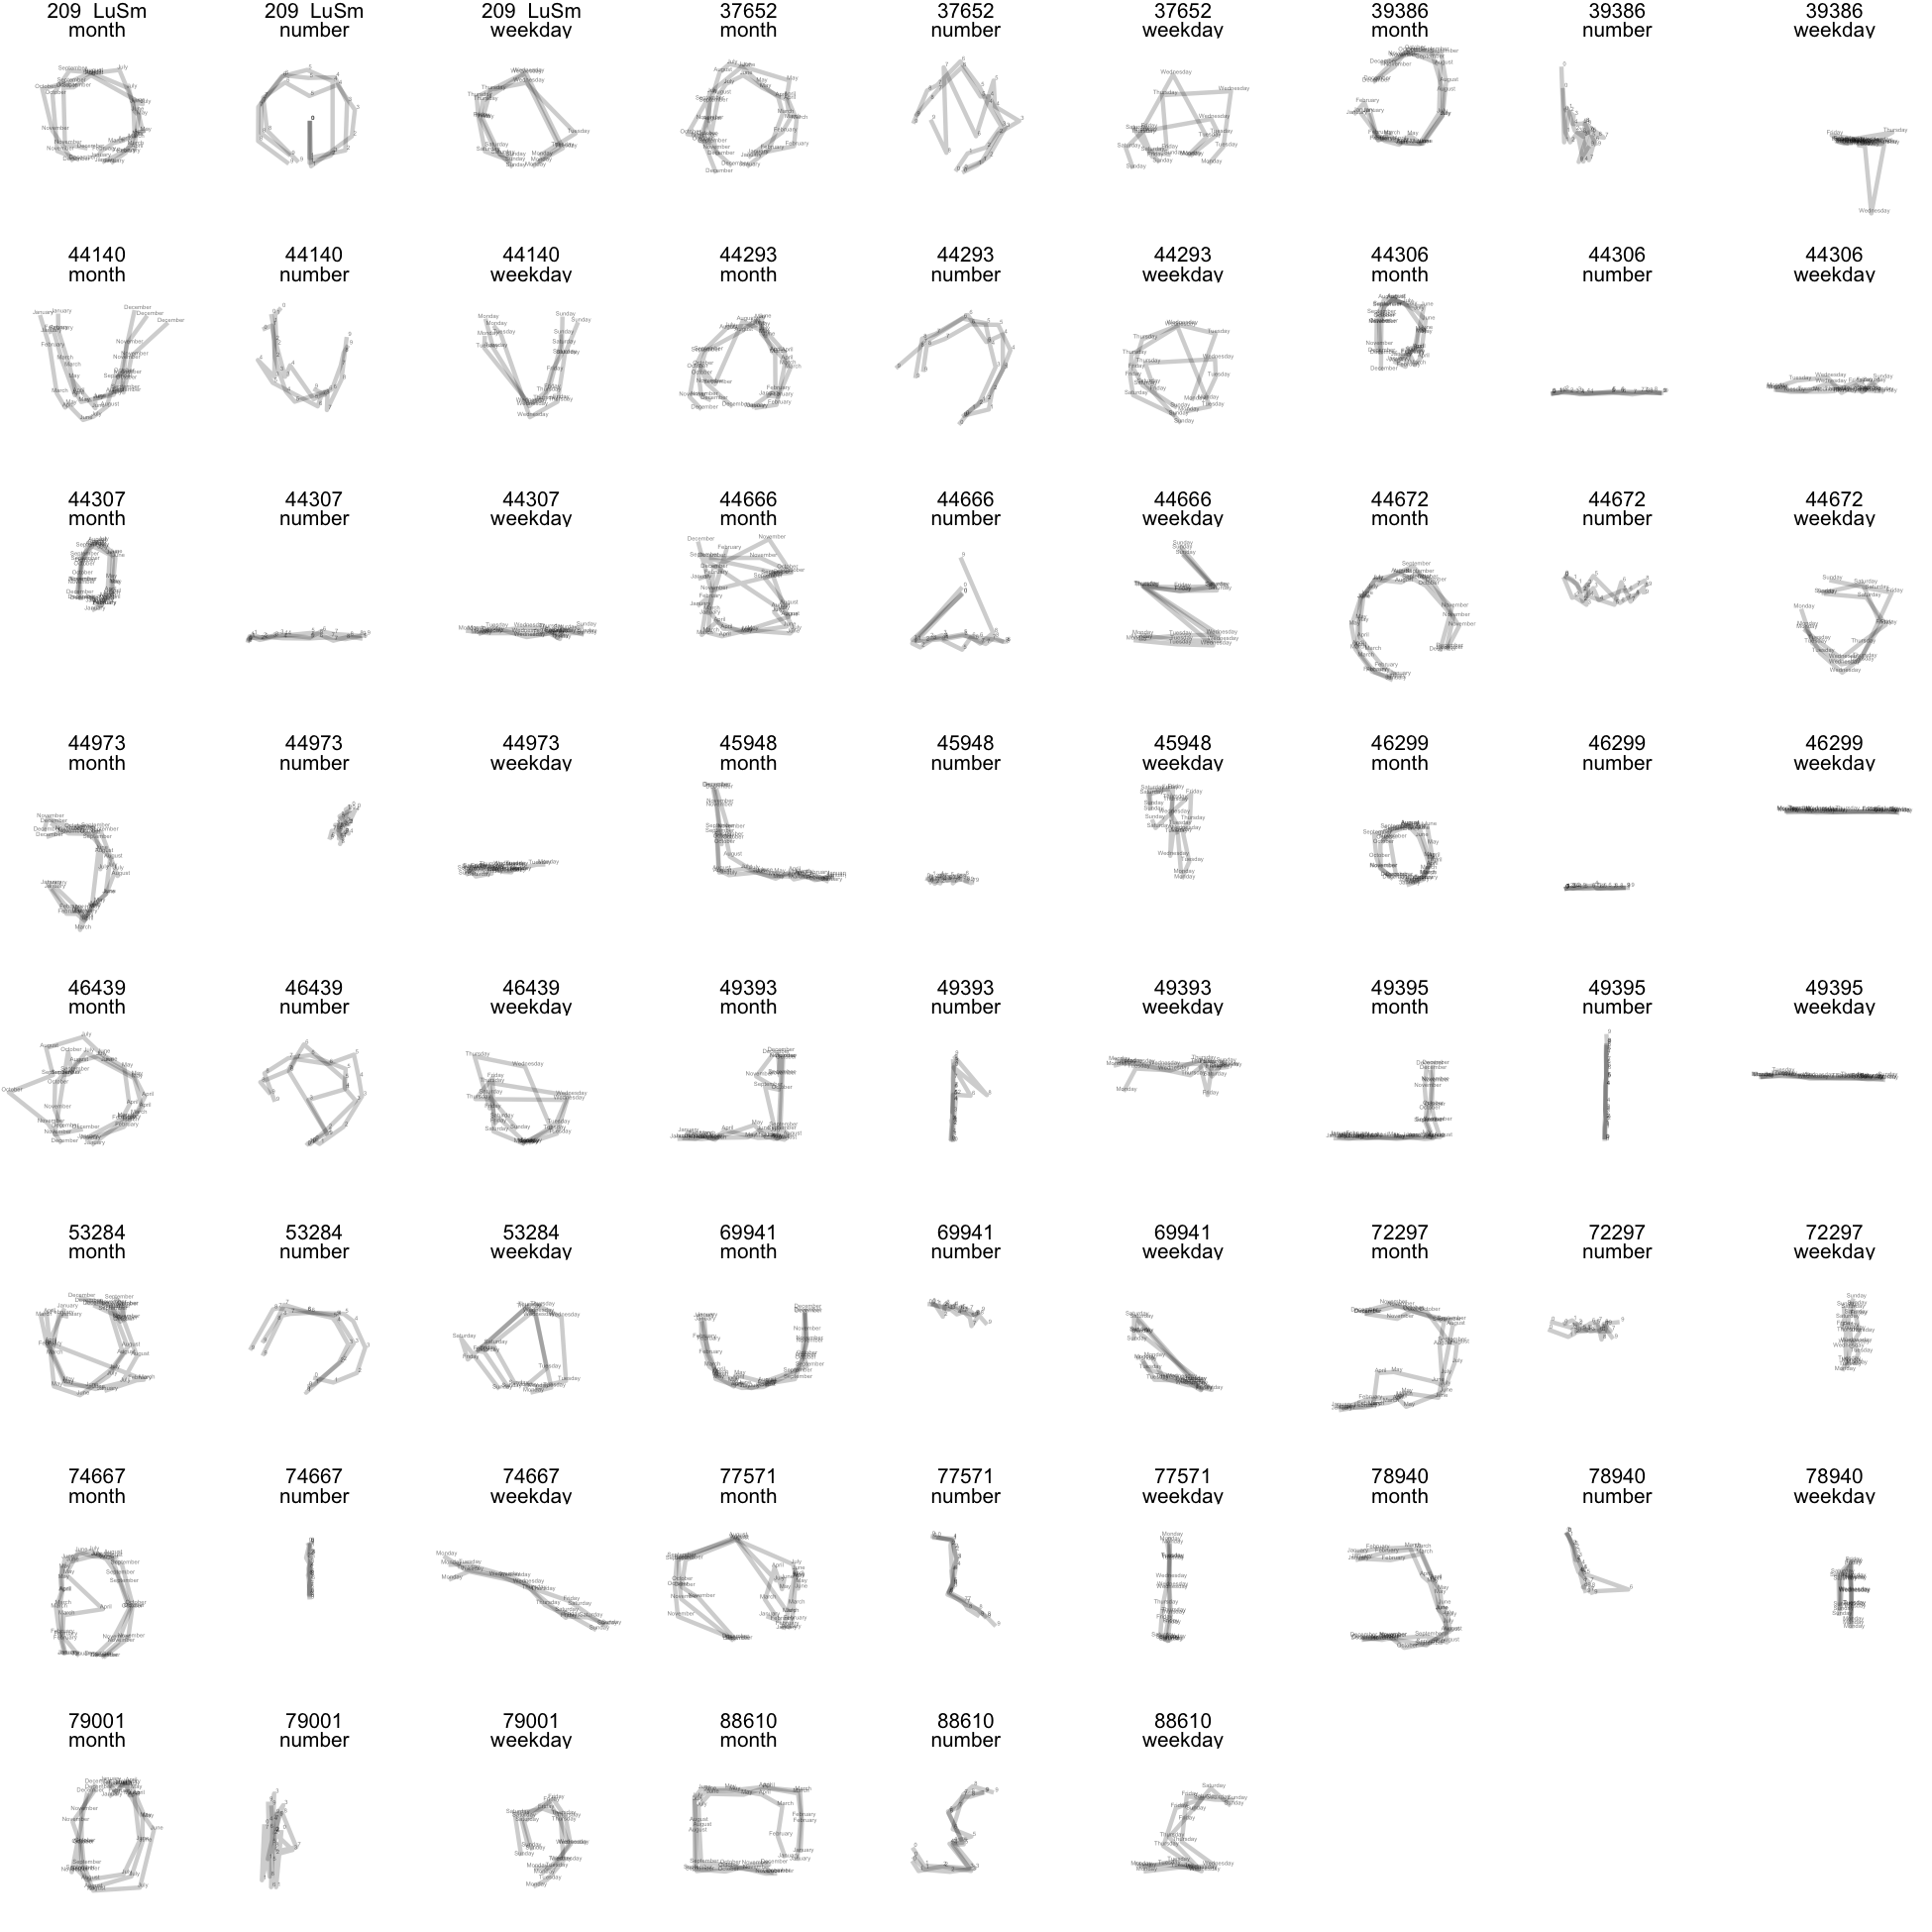
\includegraphics[keepaspectratio]{2.RegisteredReport_MS3_files/figure-pdf/fig-apx09-1.png}}

}

\end{figure}%

\section{False positive and negative
analysis}\label{apx-false-positive-and-negative-analysis}

To visualize whether one of the consistency tests is biased towards the
classification of one category, we selected the false positives and
negatives of the three best performing consistency methods (i.e.
permuted validity, polsby-popper and standardized perimeter). While
allowing only for visual comparison, the

\begin{figure}

\caption{\label{fig-apx10}For permuted validity: average forms per
categories of false positives and negatives}

\centering{

\pandocbounded{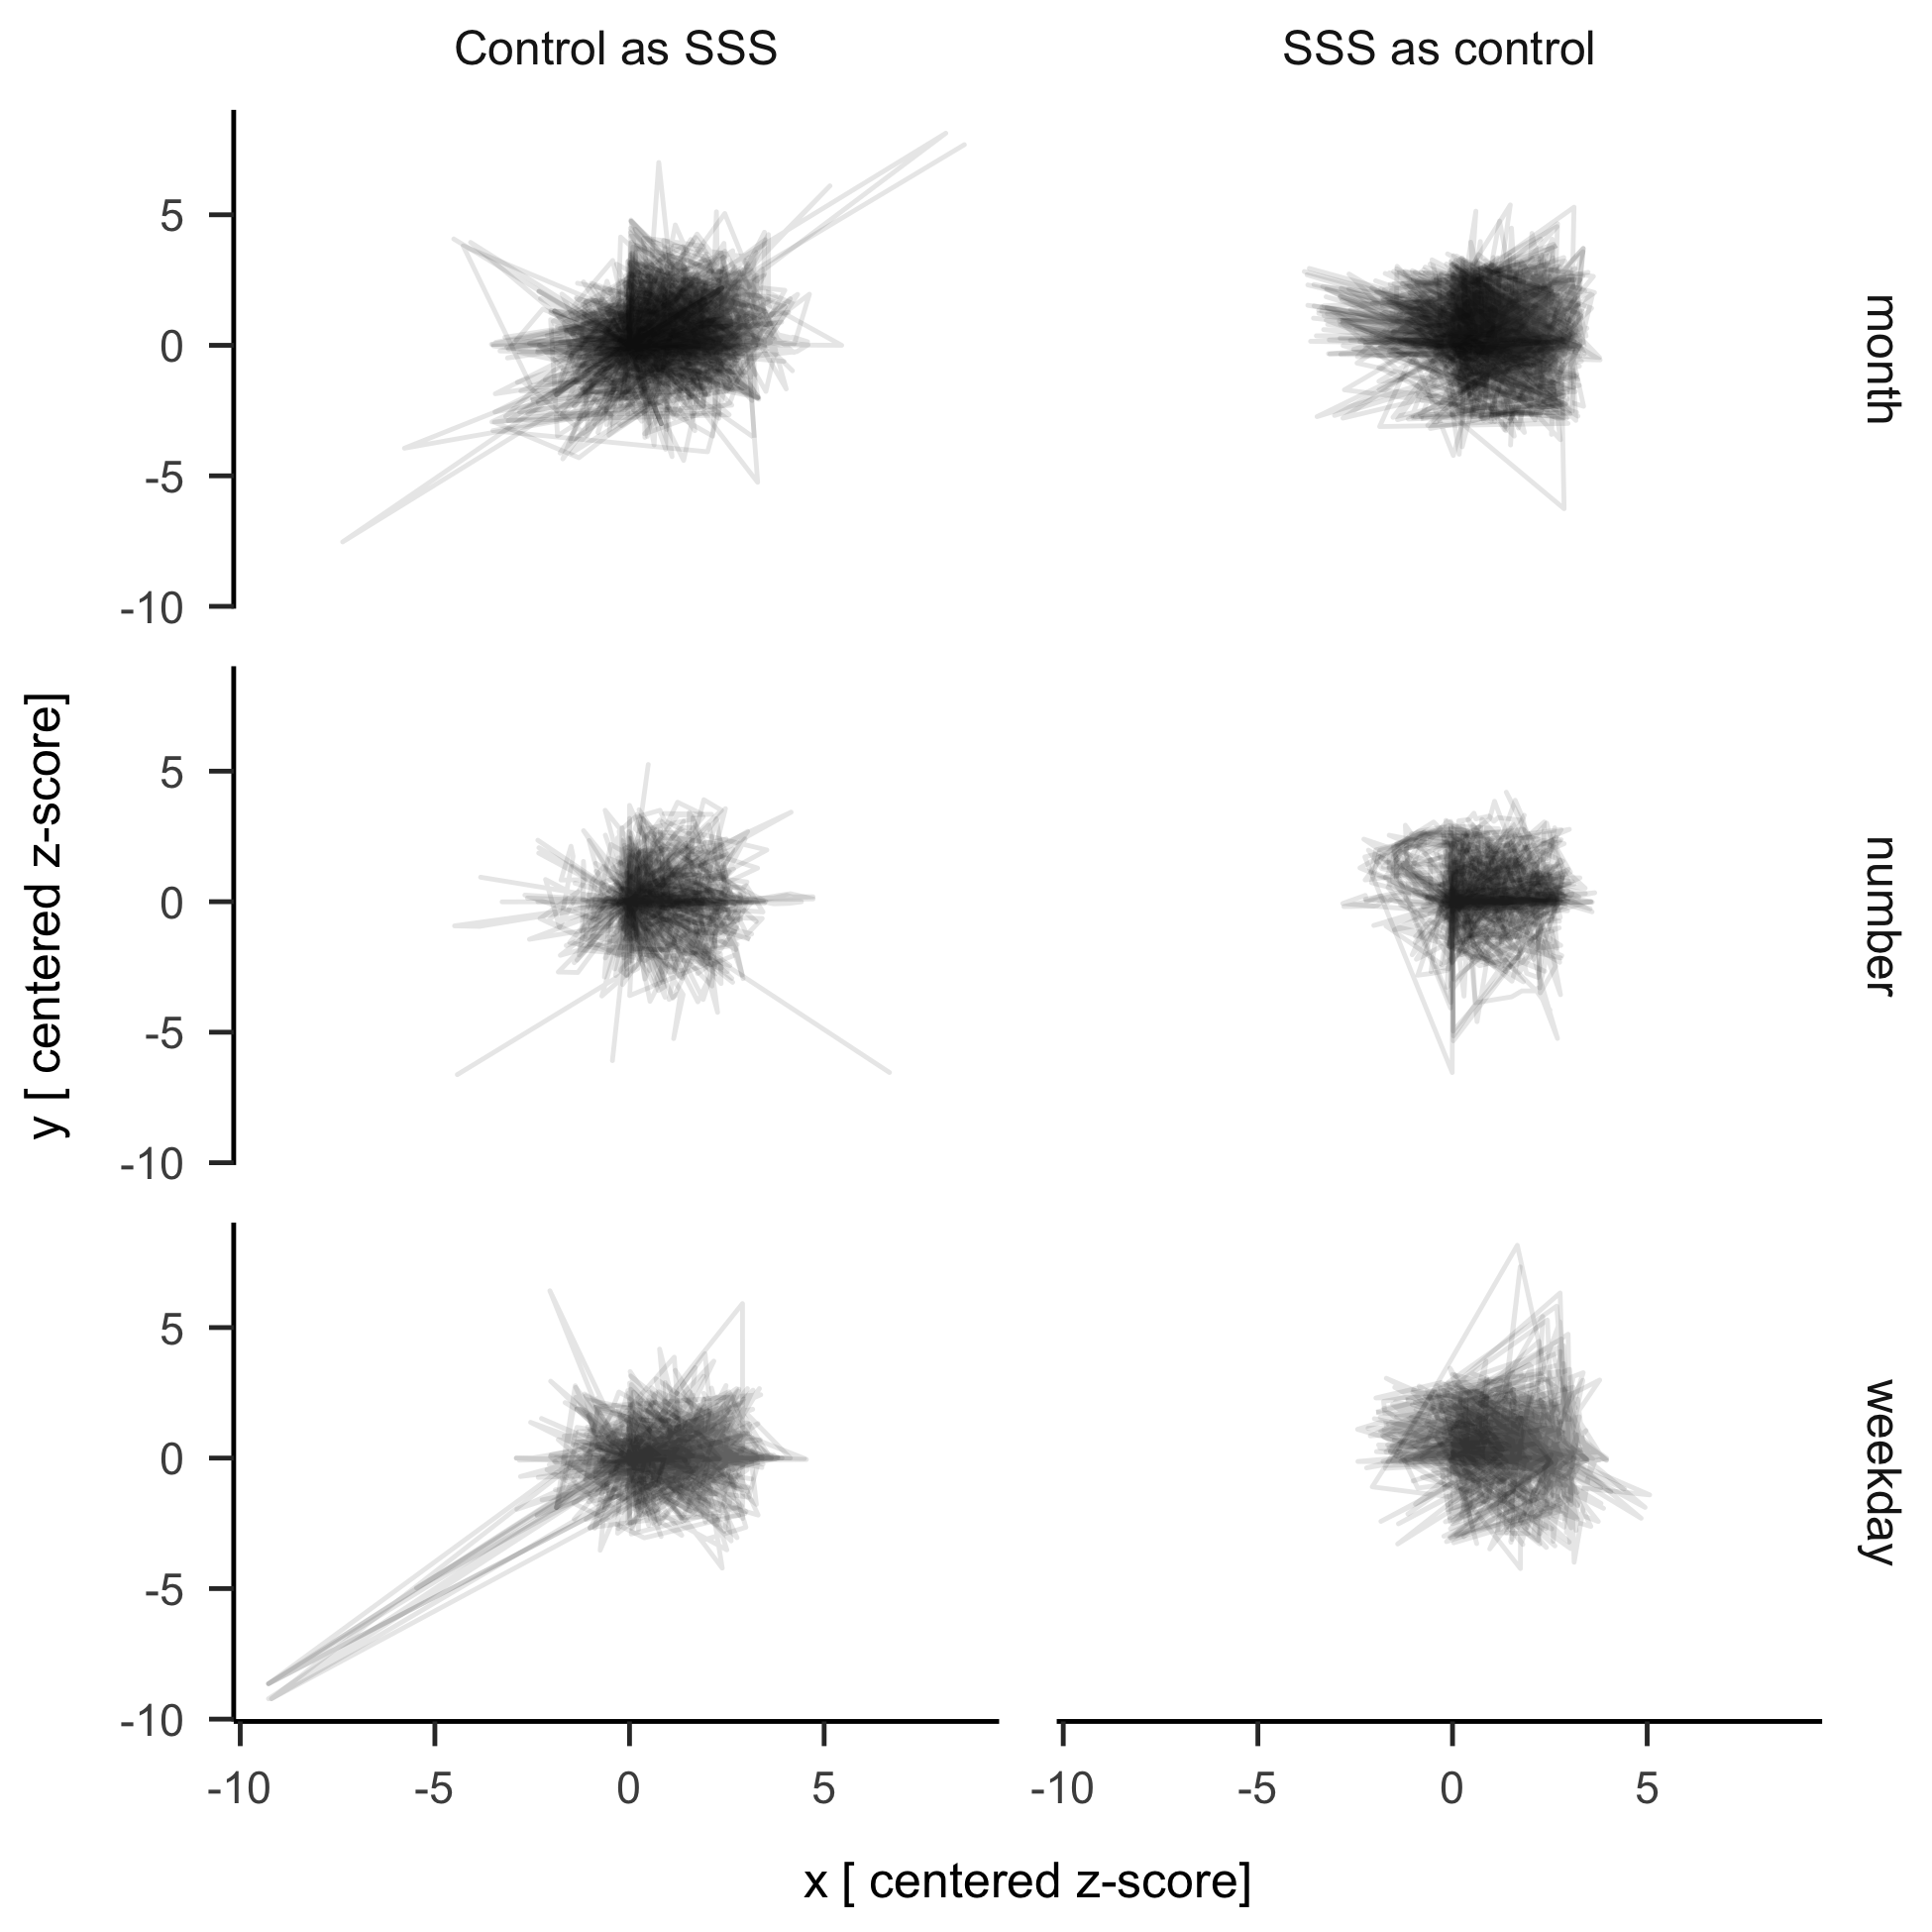
\includegraphics[keepaspectratio]{2.RegisteredReport_MS3_files/figure-pdf/fig-apx10-1.png}}

}

\end{figure}%

\begin{figure}

\caption{\label{fig-apx11}For Polsby-popper: average forms per
categories of false positives and negatives}

\centering{

\pandocbounded{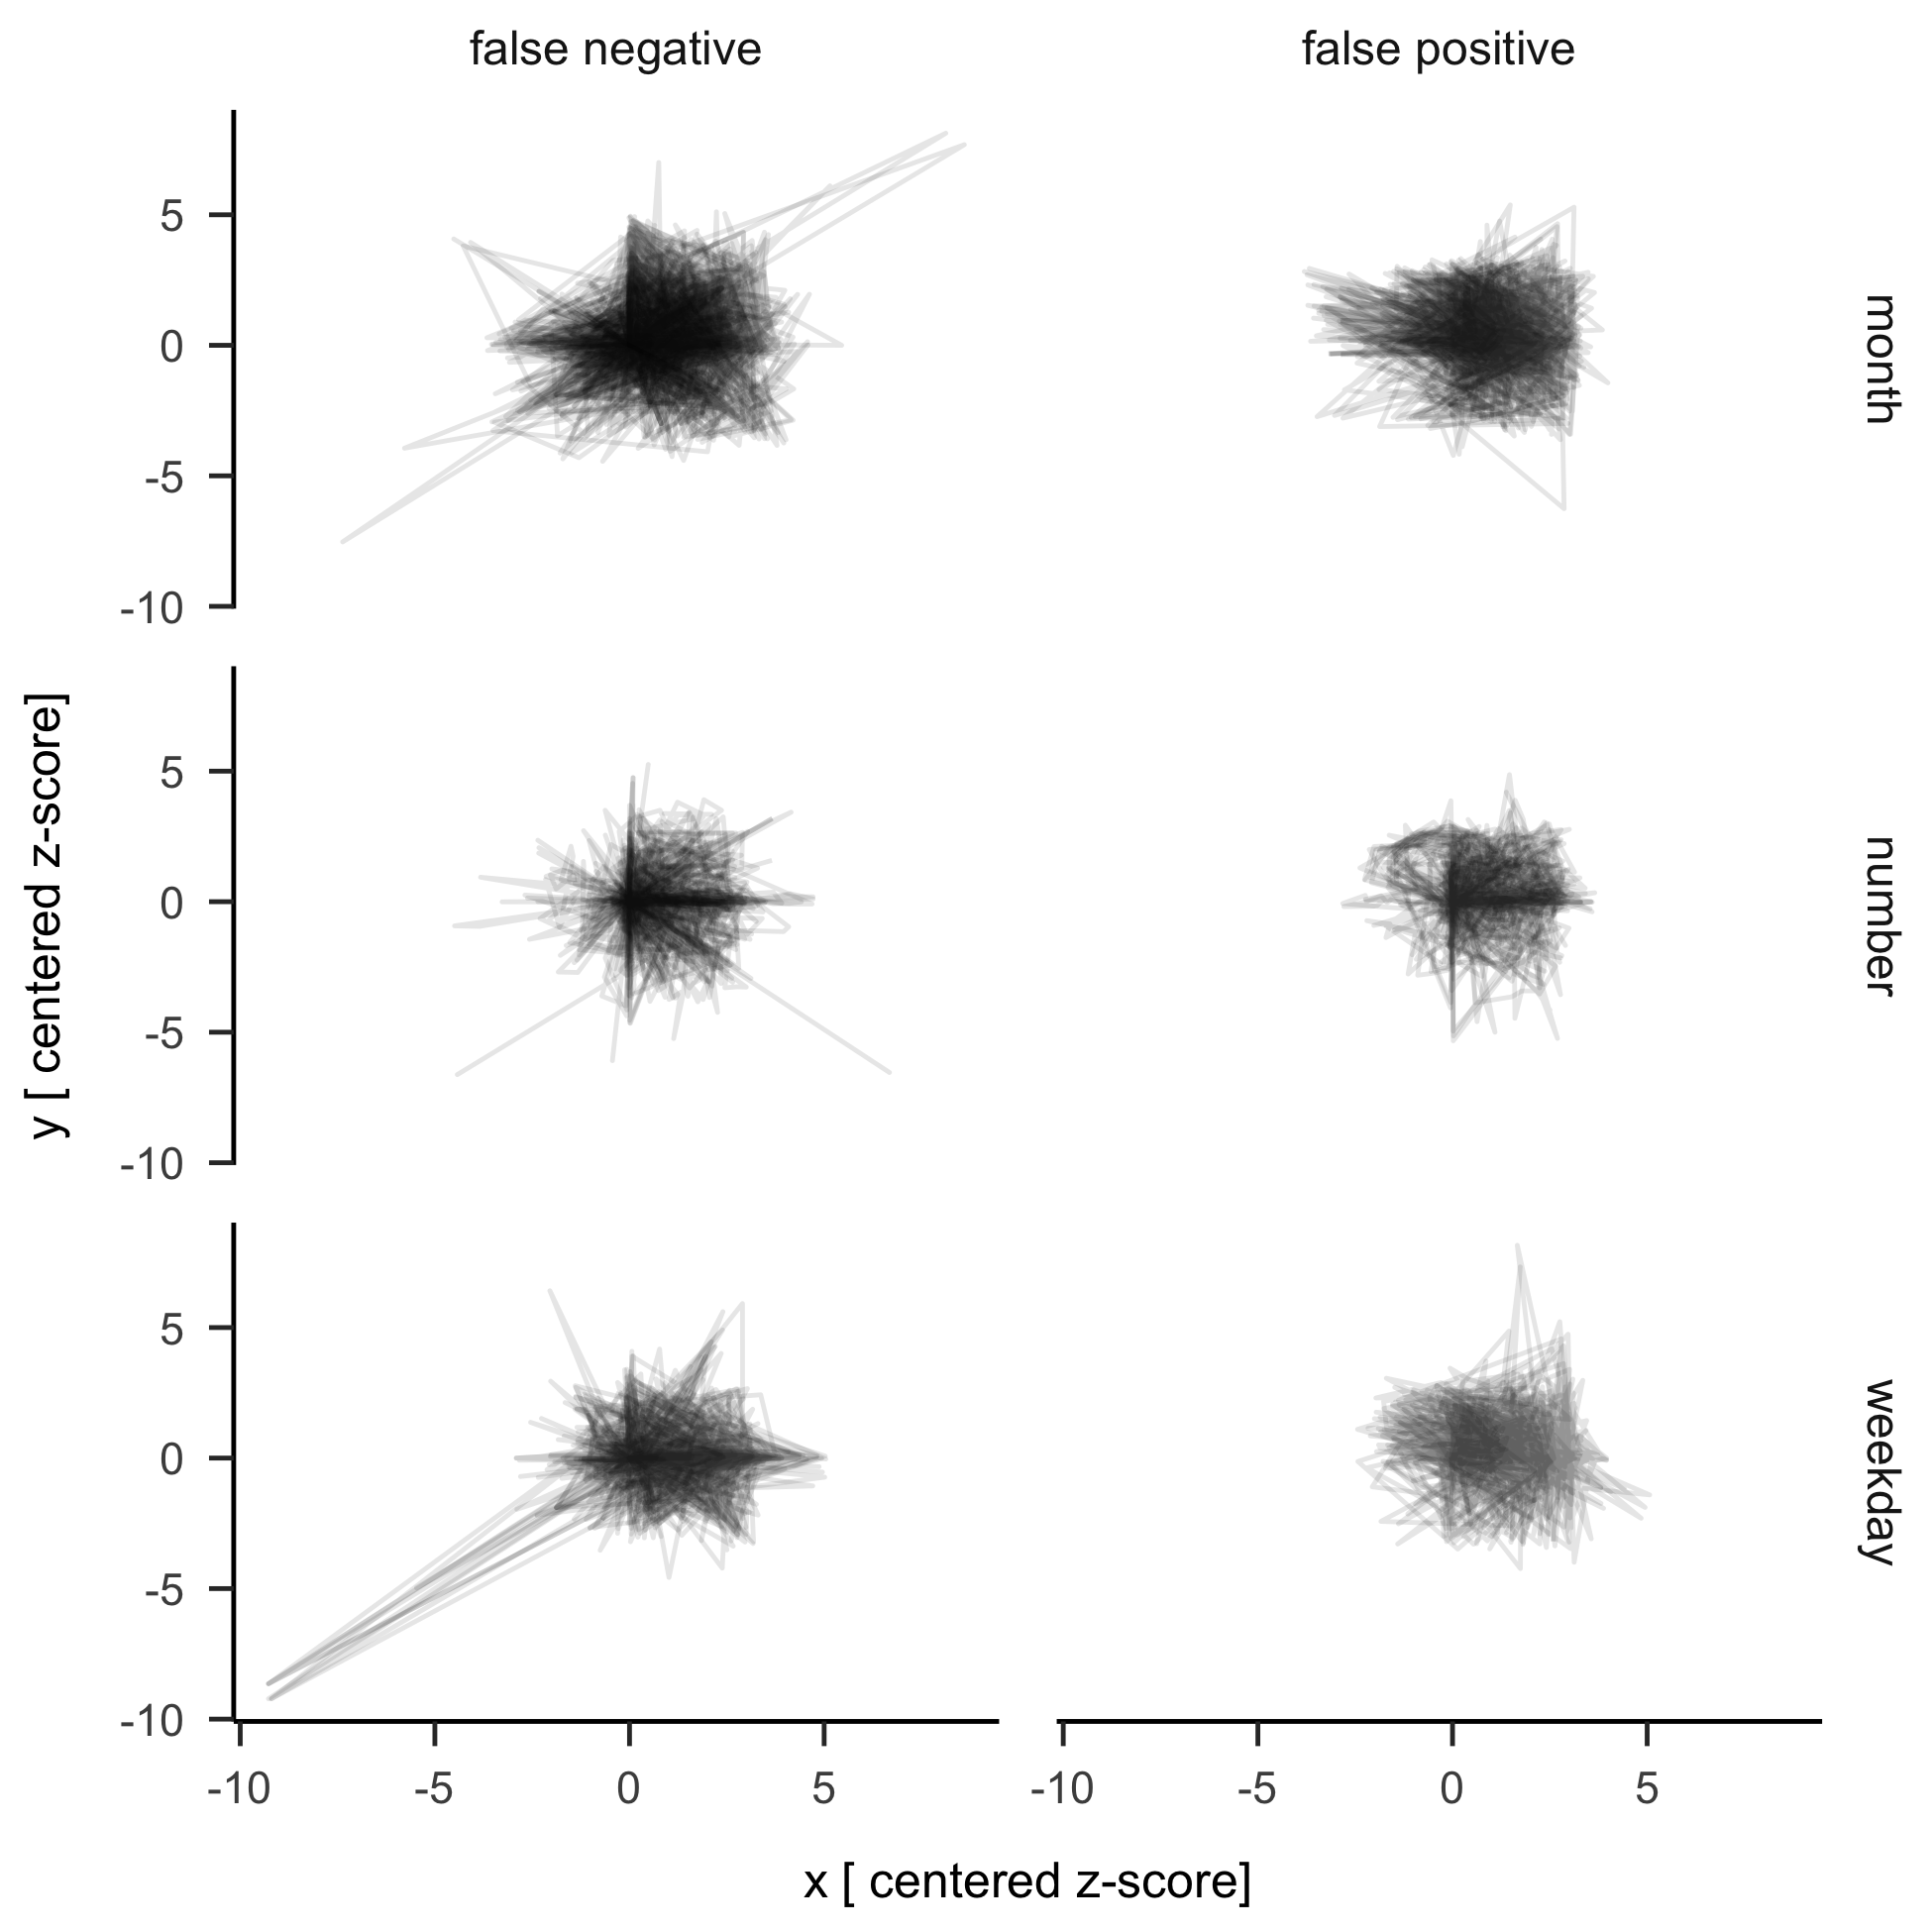
\includegraphics[keepaspectratio]{2.RegisteredReport_MS3_files/figure-pdf/fig-apx11-1.png}}

}

\end{figure}%

\begin{figure}

\caption{\label{fig-apx12}For perimeter: average forms per categories of
false positives and negatives}

\centering{

\pandocbounded{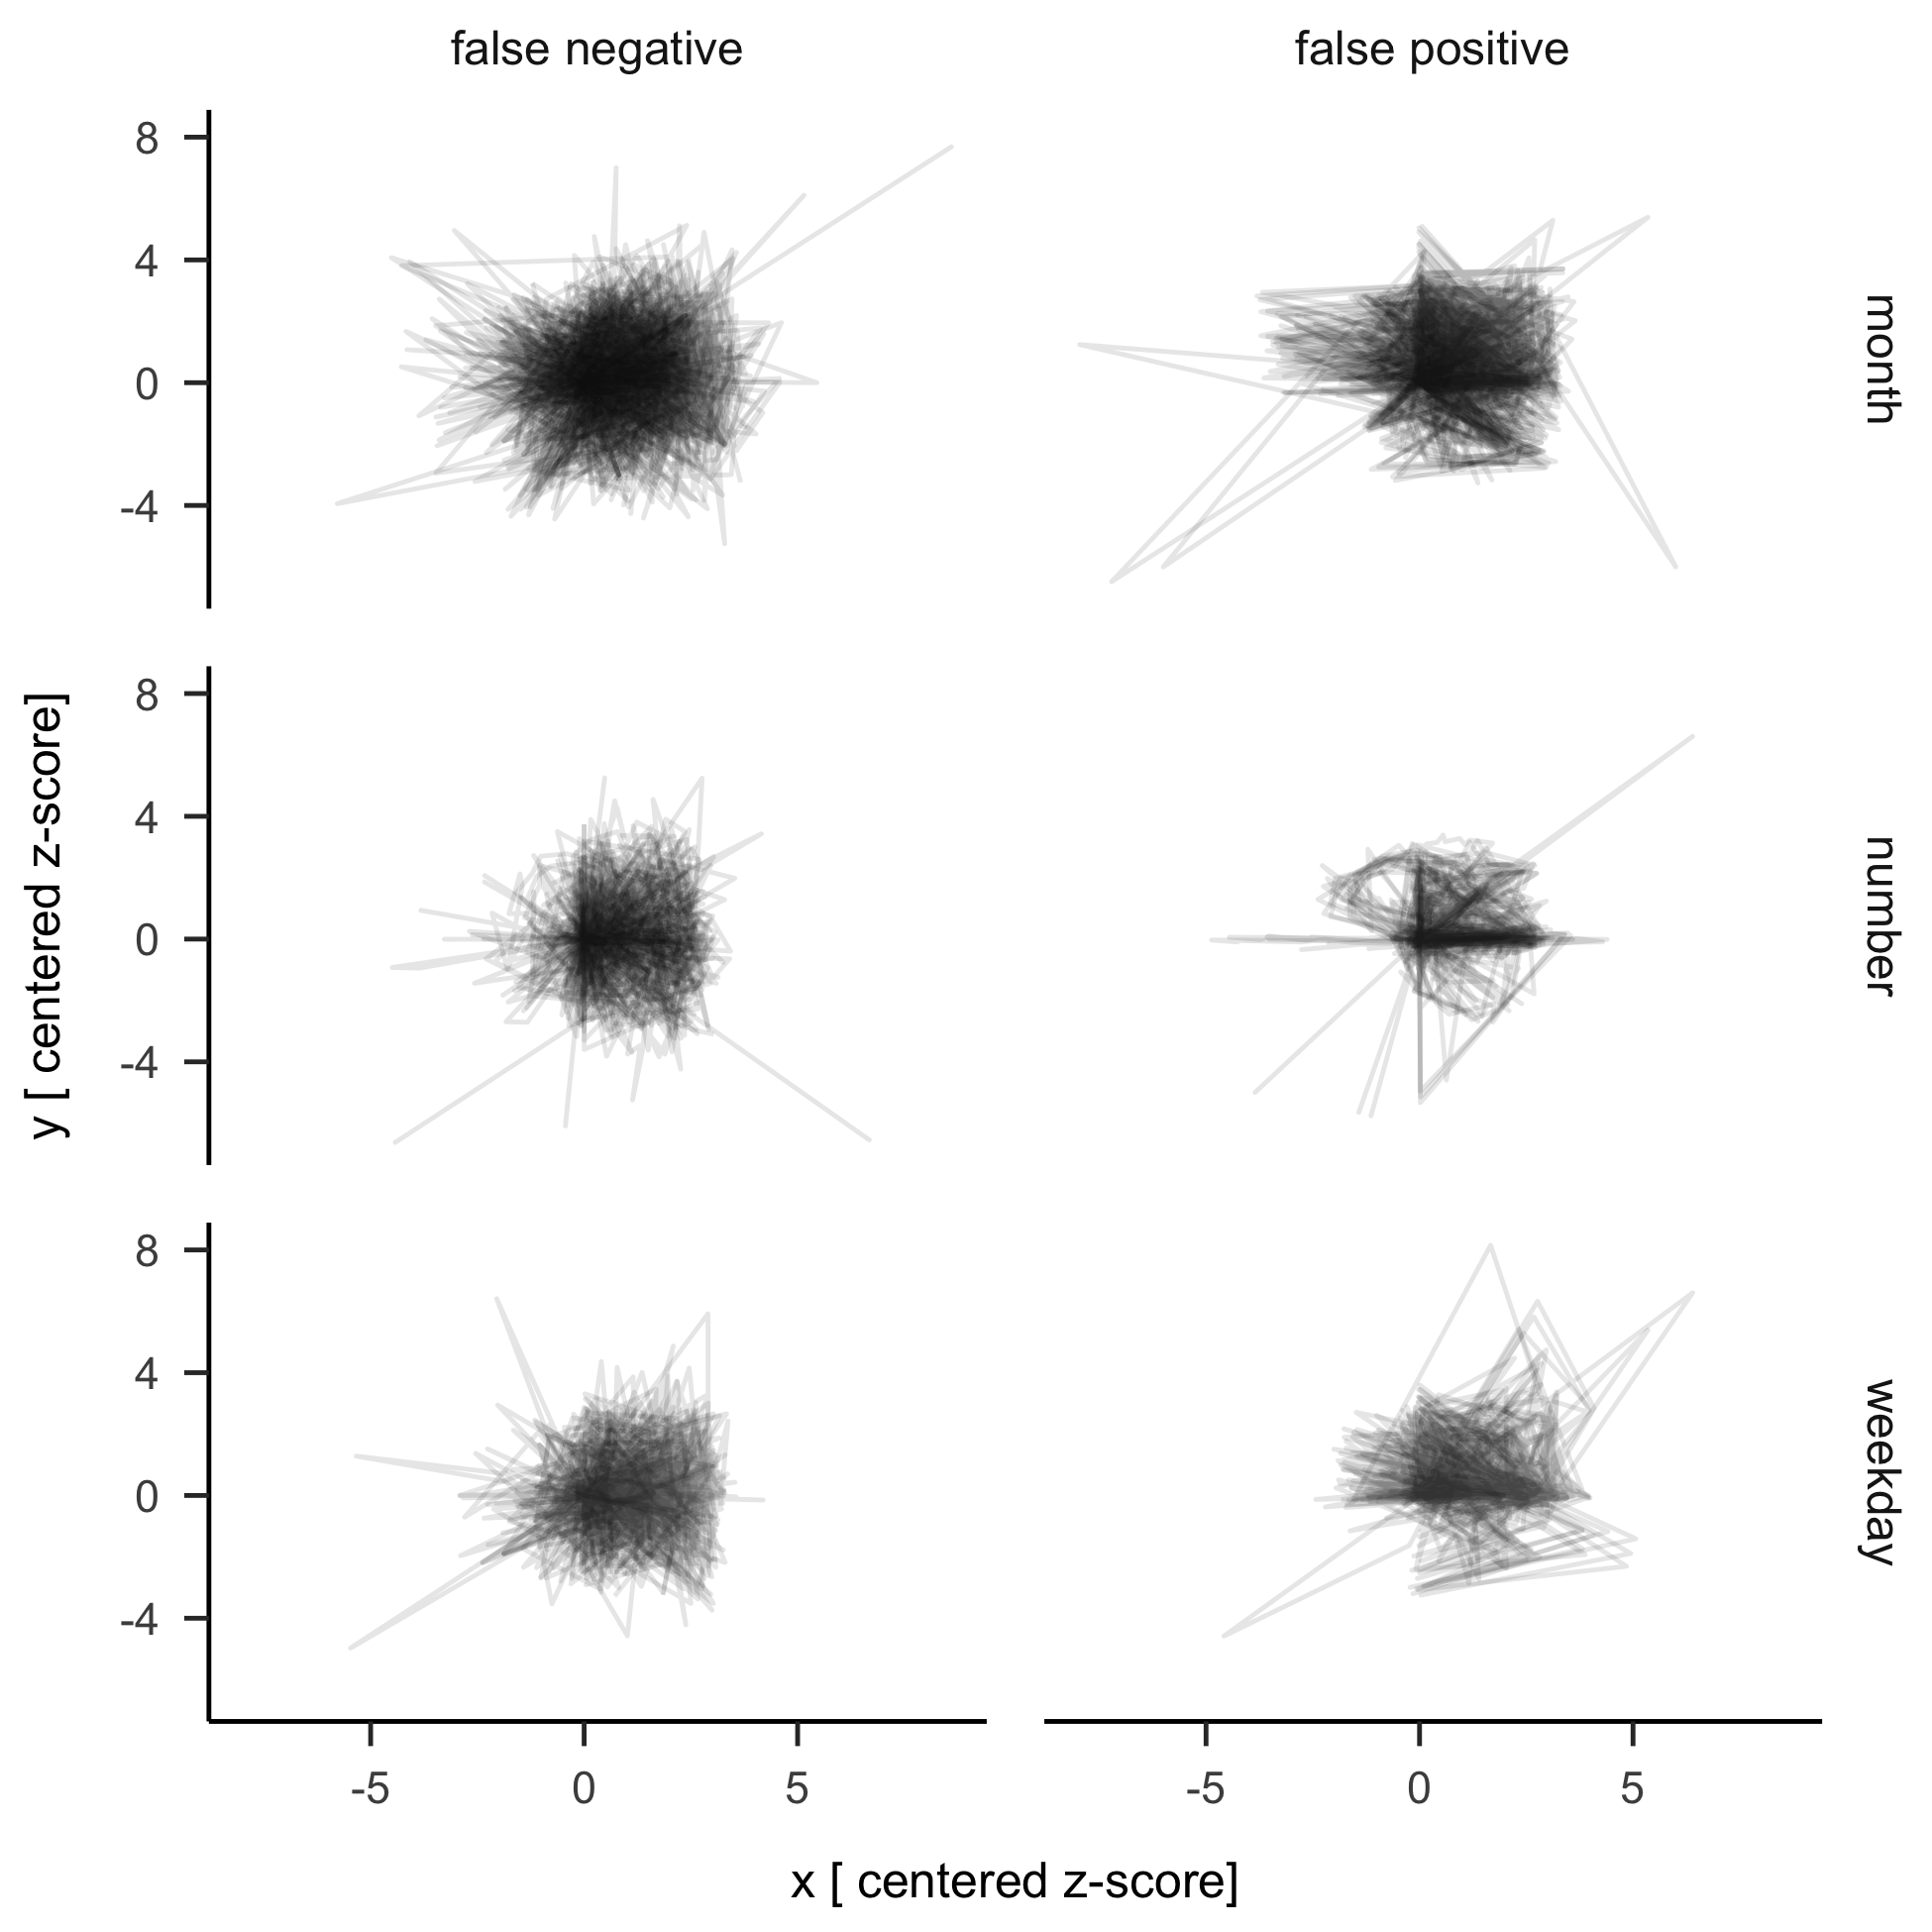
\includegraphics[keepaspectratio]{2.RegisteredReport_MS3_files/figure-pdf/fig-apx12-1.png}}

}

\end{figure}%

\section{All participants spatial
forms}\label{apx-all-participants-spatial-forms}

Here we report the code to plot each participant and categories in
z-score x and y coordinates. At the top right corner, the first coloured
dot indicates if the participant self-reports as SSS (green) or not
(red). The following dots indicates if the participant passes (green) or
fails (red) the given consistency test.






\end{document}
